%----------------------------------------------------------------------------------------
%	PACKAGES AND OTHER DOCUMENT CONFIGURATIONS
%----------------------------------------------------------------------------------------

\documentclass[
11pt, % The default document foCnt size, options: 10pt, 11pt, 12pt
oneside, % Two side (alternating margins) for binding by default, uncomment to switch to one side
ngerman, % ngerman for German
singlespacing, % Single line spacing, alternatives: onehalfspacing or doublespacing
%draft, % Uncomment to enable draft mode (no pictures, no links, overfull hboxes indicated)
%nolistspacing, % If the document is onehalfspacing or doublespacing, uncomment this to set spacing in lists to single
%liststotoc, % Uncomment to add the list of figures/tables/etc to the table of contents
%toctotoc, % Uncomment to add the main table of contents to the table of contents
%parskip, % Uncomment to add space between paragraphs
%nohyperref, % Uncomment to not load the hyperref package
headsepline, % Uncomment to get a line under the header
%chapterinoneline, % Uncomment to place the chapter title next to the number on one line
%consistentlayout, % Uncomment to change the layout of the declaration, abstract and acknowledgements pages to match the default layout
]{MasterThesis} % The class file specifying the document structure

\usepackage[utf8]{inputenc} % Required for inputting international characters
\usepackage[T1]{fontenc} % Output font encoding for international characters

\usepackage{mathpazo} % Use the Palatino font by default

\usepackage[backend=bibtex,natbib=true]{biblatex} % Use the bibtex backend with the authoryear citation style (which resembles APA) removed: style=authoryear,

\addbibresource{bibliography.bib} % The filename of the bibliography

\usepackage[autostyle=true]{csquotes} % Required to generate language-dependent quotes in the bibliography

\usepackage{caption}
\usepackage{framed} % rahmen um abbildungen
\usepackage{enumerate}

\usepackage{float} % um bilder fest zu positionieren mittels H

% Für Logo auf Titelseite %
\usepackage[absolute]{textpos}	% Bilder absolut positionieren. 
\setlength{\TPHorizModule}{1mm}
\setlength{\TPVertModule}{\TPHorizModule}
\textblockorigin{0mm}{0mm}
% %%%%%%%%%%%%%%%%%%%%%%% %

\usepackage[draft]{todonotes} %display
%\usepackage[disable]{todonotes} % do not display TODOs

% Mathepakete
\usepackage{amsfonts}
\usepackage{amsmath}

% For java code snippets 

\usepackage{color}

\definecolor{pblue}{rgb}{0.13,0.13,1}
\definecolor{pgreen}{rgb}{0,0.5,0}
\definecolor{pred}{rgb}{0.9,0,0}
\definecolor{pgrey}{rgb}{0.46,0.45,0.48}

\usepackage{listings}
\lstset{language=Java,
  showspaces=false,
  showtabs=false,
  breaklines=true,
  numbers=left,
  showstringspaces=false,
  breakatwhitespace=true,
  commentstyle=\color{pgreen},
  keywordstyle=\color{pblue},
  stringstyle=\color{pred},
  basicstyle=\ttfamily,
  moredelim=[il][\textcolor{pgrey}]{\$\$},
  moredelim=[is][\textcolor{pgrey}]{\%\%}{\%\%}
}

%----------------------------------------------------------------------------------------
%	MARGIN SETTINGS
%----------------------------------------------------------------------------------------

\geometry{
	paper=a4paper, % Change to letterpaper for US letter
	inner=2.5cm, % Inner margin
	outer=3.8cm, % Outer margin
	bindingoffset=.5cm, % Binding offset
	top=1.5cm, % Top margin
	bottom=1.5cm, % Bottom margin
	%showframe, % Uncomment to show how the type block is set on the page
}

%----------------------------------------------------------------------------------------
%	THESIS INFORMATION
%----------------------------------------------------------------------------------------
%
\thesistitle{Einsatz und Vergleich verschiedener Blockchain-Technologien am Beispiel einer Glücksspielanwendung} % Your thesis title, this is used in the title and abstract, print it elsewhere with \ttitle
\supervisor{Prof. Dr. rer. nat. Dr.-Ing. Georg \textsc{Hoever}} % Your supervisor's name, this is used in the title page, print it elsewhere with \supname
\examiner{} % Your examiner's name, this is not currently used anywhere in the template, print it elsewhere with \examname
\degree{Information System Engineering} % Your degree name, this is used in the title page and abstract, print it elsewhere with \degreename
\author{Dany \textsc{Brossel}} % Your name, this is used in the title page and abstract, print it elsewhere with \authorname
\addresses{} % Your address, this is not currently used anywhere in the template, print it elsewhere with \addressname

\subject{IT} % Your subject area, this is not currently used anywhere in the template, print it elsewhere with \subjectname
\keywords{} % Keywords for your thesis, this is not currently used anywhere in the template, print it elsewhere with \keywordnames
\university{\href{http://www.fh-aachen.de}{FH Aachen}} % Your university's name and URL, this is used in the title page and abstract, print it elsewhere with \univname
\department{\href{http://department.university.com}{Fachbereich 5}} % Your department's name and URL, this is used in the title page and abstract, print it elsewhere with \deptname
\group{\href{http://researchgroup.university.com}{Research Group Name}} % Your research group's name and URL, this is used in the title page, print it elsewhere with \groupname
\faculty{\href{https://www.fh-aachen.de/fachbereiche/elektrotechnik-und-informationstechnik/}{Fachbereich Name}} % Your faculty's name and URL, this is used in the title page and abstract, print it elsewhere with \facname

\AtBeginDocument{
\hypersetup{pdftitle=\ttitle} % Set the PDF's title to your title
\hypersetup{pdfauthor=\authorname} % Set the PDF's author to your name
\hypersetup{pdfkeywords=\keywordnames} % Set the PDF's keywords to your keywords
}

\begin{document}

\frontmatter % Use roman page numbering style (i, ii, iii, iv...) for the pre-content pages

\pagestyle{plain} % Default to the plain heading style until the thesis style is called for the body content

%----------------------------------------------------------------------------------------
%	TITLE PAGE
%----------------------------------------------------------------------------------------



\begin{titlepage}
\thispagestyle{empty}%
\setlength{\oddsidemargin}{0cm}%
\enlargethispage{\baselineskip}
\begin{textblock}{16}(188,8)%
    
\includegraphics[width=1.5cm]{Figures/fh_logo_rechts.png}%
\end{textblock}%
\vspace*{-1.0cm}
\noindent
\LARGE\textbf{\univname}\\
%\Large\textbf{UNIVERSITY OF APPLIED SIENCES}\\
\Large\textbf{Fachbereich Elektrotechnik und Informationstechnik}\\
%\large \href{https://www.fh-aachen.de/menschen/hoever/}{\supname} 
\vspace{2cm}
\begin{center}
	\LARGE\textbf{Masterarbeit}\\
	\vspace{1.75cm}
	\LARGE \ttitle\\
	\large
	\vspace{2.5cm}
	Eingereicht von:\\
	{\authorname}\\
	Matrikelnummer: 3024062\\
	\vspace{1.5cm}
	Studiengang: Information Systems Engineering\\
	\vspace{1.5cm}
	\today\\
	\vspace{2cm}
	Betreuer: \href{https://www.fh-aachen.de/menschen/hoever/}{\supname}\\
	Korreferent: \href{https://www.fh-aachen.de/menschen/schuba/}{Prof. Dr. Marco \textsc{Schuba}}
\end{center}
\end{titlepage}

%----------------------------------------------------------------------------------------
%	DECLARATION PAGE
%----------------------------------------------------------------------------------------

\begin{declaration}
\vspace*{.04\textheight}
\noindent Ich versichere hiermit, dass ich die vorliegende Arbeit selbstständig verfasst und keine anderen als
die im Literaturverzeichnis angegebenen Quellen benutzt habe.\newline\newline
Stellen, die wörtlich oder sinngemäß aus veröffentlichten oder noch nicht veröffentlichten Quellen
entnommen sind, sind als solche kenntlich gemacht.\newline\newline
Die Zeichnungen oder Abbildungen in dieser Arbeit sind von mir selbst erstellt worden oder mit
einem entsprechenden Quellennachweis versehen.\newline\newline
Diese Arbeit ist in gleicher oder ähnlicher Form noch bei keiner anderen Prüfungsbehörde eingereicht
worden.\newline\newline\newline

\noindent Datum:\\
\rule[0.5em]{25em}{0.5pt} % This prints a line to write the date


\noindent Unterschrift:\\
\rule[0.5em]{25em}{0.5pt} % This prints a line for the signature
 
\end{declaration}

\cleardoublepage

%----------------------------------------------------------------------------------------
%	QUOTATION PAGE
%----------------------------------------------------------------------------------------

%\vspace*{0.2\textheight}

%\noindent\enquote{\itshape Thanks to my solid academic training, today I can write hundreds of words on virtually any topic without possessing a shred of information, which is how I got a good job in journalism.}\bigbreak

%\hfill Dave Barry

%----------------------------------------------------------------------------------------
%	ABSTRACT PAGE
%----------------------------------------------------------------------------------------

\begin{abstract}
\addchaptertocentry{\abstractname} % Add the abstract to the table of contents

Diese Zusammenfassung werde ich erst am Ende schreiben. Also nicht die Idee beschreiben, sondern eher zusammengefasst, was gemacht wurde und welche Resultate aus der Arbeit hervorgehen.

\end{abstract}

%----------------------------------------------------------------------------------------
%	ACKNOWLEDGEMENTS
%----------------------------------------------------------------------------------------

%\begin{acknowledgements}
%\addchaptertocentry{\acknowledgementname} % Add the acknowledgements to the table of contents
%The acknowledgments and the people to thank go here, don't forget to include your project advisor\ldots
%\end{acknowledgements}

%----------------------------------------------------------------------------------------
%	Table of content
%----------------------------------------------------------------------------------------

\setcounter{tocdepth}{2}
\tableofcontents % Prints the main table of contents


%----------------------------------------------------------------------------------------
%	ABBREVIATIONS
%----------------------------------------------------------------------------------------

\begin{abbreviations}{ll} % Include a list of abbreviations (a table of two columns)
\textbf{ECDSA} & \textbf{E}lliptic \textbf{C}urve \textbf{D}igital \textbf{S}ignature \textbf{A}lgorithm\\
\textbf{ASIC} & \textbf{A}pplication \textbf{S}pecific \textbf{I}ntegrated \textbf{C}ircuit\\
\textbf{BIP} & \textbf{B}itcoin  \textbf{I}mprovement \textbf{P}roposal\\
\textbf{GUI} & \textbf{G}raphical \textbf{U}ser \textbf{I}nterface\\
\textbf{RPC} & \textbf{R}emote  \textbf{P}rocedure \textbf{C}all\\
\textbf{EIP} & \textbf{E}thereum  \textbf{I}mprovement \textbf{P}roposal\\
\textbf{ABI} & \textbf{A}pplication  \textbf{B}inary \textbf{I}nterface\\
\textbf{JSON} & \textbf{J}avaScript \textbf{O}bject \textbf{No}tation\\
\textbf{DAG} & \textbf{D}irected \textbf{A}cyclic \textbf{G}raph\\
\textbf{SPV} & \textbf{S}implified \textbf{P}ayment \textbf{V}erification\\  
\textbf{JVM} & \textbf{J}ava \textbf{V}irtual \textbf{M}achine\\ 
\end{abbreviations}

%----------------------------------------------------------------------------------------
%	PHYSICAL CONSTANTS/OTHER DEFINITIONS
%----------------------------------------------------------------------------------------

%\begin{constants}{lr@{${}={}$}l} % The list of physical constants is a three column table

% The \SI{}{} command is provided by the siunitx package, see its documentation for instructions on how to use it

%Speed of Light & $c_{0}$ & \SI{2.99792458e8}{\meter\per\second} (exact)\\
%Constant Name & $Symbol$ & $Constant Value$ with units\\

%\end{constants}

%----------------------------------------------------------------------------------------
%	SYMBOLS
%----------------------------------------------------------------------------------------

%\begin{symbols}{lll} % Include a list of Symbols (a three column table)

%$a$ & distance & \si{\meter} \\
%$P$ & power & \si{\watt} (\si{\joule\per\second}) \\
%Symbol & Name & Unit \\

%\addlinespace % Gap to separate the Roman symbols from the Greek

%$\omega$ & angular frequency & \si{\radian} \\

%\end{symbols}

%----------------------------------------------------------------------------------------
%	DEDICATION
%----------------------------------------------------------------------------------------

%\dedicatory{For/Dedicated to/To my\ldots} 

%----------------------------------------------------------------------------------------
%	THESIS CONTENT - CHAPTERS
%----------------------------------------------------------------------------------------

\mainmatter % Begin numeric (1,2,3...) page numbering

\pagestyle{thesis} % Return the page headers back to the "thesis" style

% Include the chapters of the thesis as separate files from the Chapters folder
% Uncomment the lines as you write the chapters

\chapter{Einleitung} % Main chapter title
\label{Chapter1}
%----------------------------------------------------------------------------------------
\newcommand{\keyword}[1]{\textbf{#1}}
\newcommand{\tabhead}[1]{\textbf{#1}}
\newcommand{\code}[1]{\texttt{#1}}
\newcommand{\file}[1]{\texttt{\bfseries#1}}
\newcommand{\option}[1]{\texttt{\itshape#1}}
%----------------------------------------------------------------------------------------
Die Erfindung der Kryptowährung Bitcoin und deren inhärente Blockchain-Technologie hat in den letzten Jahren einen regelrechten Hype ausgelöst. Begriffe wie Blockchain, Distributed Ledger und Smart Contract sind das bestimmende Thema schlechthin. 
Blockchain-Technologie verspricht, durch den Einsatz von Dezentralität, Unveränderlichkeit und Transparenz, die Möglichkeit zwischen anonymen, sich gegenseitig nicht trauenden, Parteien digitale Werte auszutauschen.

\section{Motivation}
Das Internet vernetzt weltweit mehrere Millionen Menschen. Es ermöglicht diesen anonym zu kommunizieren und miteinander zu interagieren. Aufgrund der Anonymität und des damit einhergehenden Betrugspotential, benötigen die meisten Anwendungsfälle eine sogenannte Trusted Third Party als Mittelsmann. Das fehlende Vertrauen zwischen den anonym agierenden Parteien wird durch diese dritte, nicht anonym auftretende, Partei kompensiert. Diese nicht anonyme Partei muss sich den länderspezifischen Regeln und Gesetzen unterwerfen und kann mit ihrem Service daher nur in einem gewissen, vorgegebenen Rahmen betreiben. Da das Betreiben eines solchen Services mit gewissen Kosten verbunden ist, werden diese meist auf die Nutzer abgewälzt. 

Online Casinos sind ein Beispiel für eine solche Trusted Third Party. Diese bieten eine Plattform, die Spieler vernetzt und vor gegenseitigem Betrug schützt. Außerdem verwalten Online Casinos das Geld ihrer Spieler. Die Spieler vertrauen den Casinos diese Aufgabe an, da es sich um registrierte Firmen handelt, die juristisch haftbar gemacht werden können. Ein weiterer Aspekt bei dem Vertrauen eine Rolle spielt sind die angebotenen Spiele selbst. Egal ob Black Jack, Poker oder Roulette, die meisten solcher Spiele erfordern die Generierung von Zufallszahlen. Beispielsweise wenn Spielkarten verteilt werden. Die Spieler haben dabei keine Möglichkeit nachzuprüfen, ob der Algorithmus, der ihnen die Karten zuteilt, auch wirklich fair ist. Die Spieler müssen dem Casino somit vertrauen, dass dieses sie nicht benachteiligt. 

%Der Endnutzer wird somit durch Transparenz und nicht durch staatliche Regulierungen geschützt. 
\section{Ziel}
Ziel dieser Masterarbeit ist es den Einsatz von Blockchain-Technologie an der beispielhaften Realisierung einer Glücksspielanwendung zu demonstrieren. Der Einsatz einer Blockchain soll dabei das Vertrauen, das der Endnutzer der Anwendung entgegenbringen muss, auf ein Minimum reduzieren. Falls möglich soll vollständig auf den Einsatz einer Trusted Third Party verzichtet werden.


%Das Ziel von Blockchains ist es durch transparente Systeme, die Interaktionen zwischen sich misstrauenden Parteien zu ermöglichen ohne, dass dabei das Vertrauen in eine Drittpartei erforderlich ist.

% Hier ein paar unwissenschaftliche Gründe warum 
%Als Spieler muss man sich erst registrieren und seine Bankdaten angeben. Durch diese Registrierung gibt der Spieler seine Anonymität auf. Außerdem hat der Staat eine zentrale Stelle an die er sich wenden kann um Steuereinnahmen durch die Besteuerung von Glücksspiel zu generieren. Ein weiterer Punkt der bei derzeitig etablierten Glücksspielplattformen verbesserungswürdig ist, sind Ein- und Auszahlungen. Einzahlungen und Auszahlungen  per Banküberweisungen dauern mindestens einen Tag. Dadurch muss der Glücksspieler eine lange Zeit warten bevor er den Service nutzen kann. Auch potentielle Gewinne kann er erst nach solch einer langen Zeitdauer weiterverwenden. Heutzutage gibt es zwar Dienste wie PayPal, die schnelle Zahlungen realisieren, allerdings kostet die Integration solch eines Zahlungsmittels recht hohe Gebühren für die Glücksspielplattform. Cryptowährungen bieten in dieser Hinsicht Abhilfe, da Transaktionen innerhalb wenigen Minuten bestätigt werden. Der Glücksspieler kann beispielsweise in einem Crypto-Casino spielen und sich anschließend von seinen Gewinnen eine Pizza bei Lieferando kaufen. :) (Hier nochmal drüber nachdenken ob man die Argumente nicht wissenschaftlicher verpacken könnte)

\section{Projektidee}
Die in dieser Arbeit betrachtete Glücksspielanwendung soll ein Spiel anbieten, bei dem Teilnehmer in einen Geldtopf einzahlen und auf ein zufälliges Event wetten. Jeder der Teilnehmer soll dabei die gleichen Gewinnchancen haben. Sobald alle Teilnehmer eingezahlt haben, wird einer der Teilnehmer zufällig ausgewählt und gewinnt den gesamten Geldtopf. Der Gewinner bekommt somit seinen eigenen Einsatz als auch den Einsatz aller Mitspieler ausgezahlt. Die restlichen Teilnehmer verlieren und gehen leer aus.\\\\

\noindent Die erstmalig in Bitcoin verwendete Blockchain Technologie ist für die Entwicklung einer solchen Anwendung bestens geeignet, da sie transparente, pseudonyme Zahlungen ermöglicht. Außerdem lässt sich der für die Gewinnerauswahl benötigte Zufall durch ein in der Zukunft liegenden Zustand der Blockchain abbilden. 
Der Zufallsfaktor kommt somit direkt von der Blockchain und ist für alle Teilnehmer nachvollziehbar.

%Was genau das eigentliche Spiel für den Nutzer der Glücksspielanwendung ist, ist für diese Masterarbeit zweitrangig. Ziel dieser Masterarbeit ist es zu erforschen, welche Möglichkeiten die erstmals in Bitcoin verwendete Blockchain Technologie bietet und in wie weit durch sie das Vertrauen des Endnutzers in die Anwendung reduziert werden kann.


\section{Anforderungen}\label{anforderungen}
Die zu realisierende Glücksspielanwendung muss den folgenden Anforderungen gerecht werden.
\subsubsection{1) Transparente Einzahlungen}
Die Einzahlung jedes Endnutzers ist für jeden anderen Endnutzer nachprüfbar.
\subsubsection{2) Gewinnerauswahl durch Zufallsfaktor}
Die Auswahl des Gewinners ist von einem zufälligen Faktor abhängig, auf den weder die Anwendung noch die Endnutzer einen Einfluss haben.
\subsubsection{3) Nachprüfbarkeit des Zufallsfaktor}
Jeder Endnutzer kann die Echtheit des zufälligen Faktors eigenständig nachprüfen.
\subsubsection{4) Transparente Auszahlungen}
Die Auszahlung an den Gewinner muss transparent und somit für jeden Endnutzer nachprüfbar sein.
\subsubsection{5) Fairheit des Spiels}
Jeder Endnutzer besitzt die gleiche Gewinnwahrscheinlichkeit und niemand wird benachteiligt.

\section{Vorhandenes}

\subsection{Cyberdice Protokoll}

Einen ersten Ansatz wie man im Internet Glücksspiel ohne eine vertrauenswürdige Drittpartei betreiben kann, liefert \cite{cyberdice_paper}. Es stellt ein Kommunikationsprotokoll vor, das mit Hilfe kryptographischer Methoden sicherstellt, dass weder die Teilnehmer noch Außenstehende betrügen können. Das zum Glücksspiel verwendete Protokoll funktioniert aber nur unter der Annahme, dass es eine zentrale Institution (Bank) gibt, bei der die Teilnehmer Geld einzahlen und im Falle eines Gewinns gegen die Vorlage eines Beweises Geld ausgezahlt bekommen. Durch die Erfindung dezentraler Kryptowährungen, die auf einer für jeden einsehbaren Blockchain basieren, fällt diese vorher noch benötigte zentrale Institution weg.

%Durch die Erfindung dezentraler, Ländergrenzen überschreitender Krypto-Währungssysteme ist es möglich geworden den Einfluss des Staates zu umgehen und den Endnutzer durch die Transparenz der Glücksspielanwendung zu schützen.

\subsection{Glücksspielseiten}
Es gibt bereits Services die dezentrales, transparentes Glücksspiel mit Hilfe von Kryptowährungen umsetzen.

Die Internetseite \cite{crypto_games} bietet diverse Spiele an, bei denen die Nutzer die Möglichkeit haben mit Kryptowährungen zu bezahlen.

Die Internetseite \cite{vdice} bietet ein Würfelspiel an, das durch einen Smart Contract auf der Ethereum Plattform umgesetzt ist.

Eine genaue Beschreibung der verwendeten Verfahren zur Gewinnerauswahl befindet sich im Anhang dieser Ausarbeitung.

\section{Aufbau dieser Arbeit}
In dieser Arbeit wird zunächst Bitcoin als Beispiel einer auf Blockchain-Technologie basierenden Kryptowährung betrachtet. Anschließend wird der Einsatz von Smart Contracts mit Ethereum präsentiert. In beiden Fällen werden zunächst die relevanten Grundlagen geklärt und ein Konzept vorgestellt. Anschließend wird dieses als Glücksspielanwendung mithilfe der jeweiligen Technologie umgesetzt. Die resultierenden Glücksspielanwendungen werden letztendlich unter Zuhilfenahme der aufgestellten Anforderungen evaluiert. Nach diesem Hauptteil wird abschließend weitere Blockchain-Technologien und deren Anwendbarkeit für die Projektidee betrachtet. 

\chapter{Erster Ansatz: Bitcoin}
\label{btc}

\section{Grundlagen}
\label{btc_grundlagen}
Bei Bitcoin handelt es sich um die erste digitale, dezentral organisierte Währung. Die Idee digitaler Währungen existiert bereits seit der Erfindung des Internets. Allerdings scheiterten diese in der Vergangenheit daran, dass sie auf einen zentralen Punkt der Kontrolle angewiesen waren und somit einen Single Point of Failure beinhalteten. Die am 03. Januar 2009 gestartete digitale Währung ''Bitcoin'' schaffte es erstmalig gänzlich auf die Verwendung einer zentralen Instanz zu verzichten und somit ein verteiltes, dezentrales und sicheres digitales Zahlungssystem zu realisieren. Bitcoin wurde in dem von dem Pseudonym ''Satoshi Nakamoto'' veröffentlichen Paper ''Bitcoin: A Peer-to-Peer Electronic Cash System'' das erste Mal beschrieben. \if Der Source Code der Bitcoin Software ist öffentlich verfügbar und hat dadurch seit 2009 eine regelrechte Innovationsexplosion im Bereich der digitalen Währungen ausgelöst.\fi Bitcoin funktioniert durch das Zusammenspiel mehrerer Komponenten und besteht aus:

\begin{itemize}
\item Einem dezentralen \textit{Peer-to-Peer Netzwerk}, das mit Hilfe des Bitcoin-Protokolls kommuniziert.
\item Der \textit{Blockchain}, die eine öffentlichen Transaktionsdatenbank darstellt, die alle validen Transaktionen seit dem Start des Netzwerkes aufzeichnet.
\item Einer Menge an \textit{Konsensregeln} mit Hilfe derer Netzwerkteilnehmer eigenständig Transaktionen auf ihre Gültigkeit prüfen können.
\item Einem \textit{Proof-of-Work Algorithmus}, der es erlaubt, sich in dem globalen dezentralen Netzwerk auf den Zustand der Transaktionsdatenbank zu einigen. Das kontinuierliche Ausführen des Proof-of-Work Algorithmus wird \textit{Mining} genannt.
\end{itemize}

\subsection{Peer-to-Peer Netzwerk}
Peer-to-Peer-Netzwerke sind Netzwerke, die auf direkten Verbindungen zwischen Rechnern beruhen, ohne dass dabei einer der Rechner eine Sonderstellung einnimmt oder ein Server die Kommunikation vermittelt. In einem reinen Peer-to-Peer-Netz sind alle Computer gleichberechtigt und können sowohl Dienste in Anspruch nehmen, als auch zur Verfügung stellen. Das Peer-to-Peer-Modell ist somit grundlegend verschieden von dem im Internet am häufigsten verwendeten Client-Server-Modell. Da jeder Knoten des Netzwerks gleichzeitig Client und Server ist, gibt es keine zentrale Instanz, die einen sogenannten ''Single Point of Failure'' darstellt. 

\begin{figure}[H]
\centering
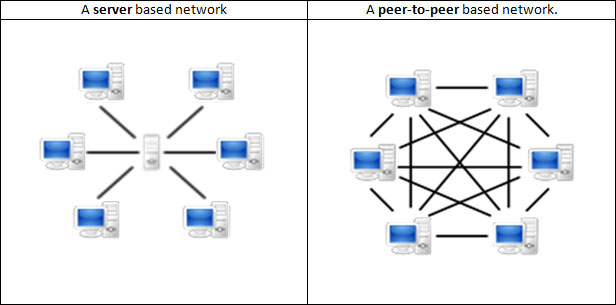
\includegraphics[width=1\linewidth]{Figures/p2p_networks}
\decoRule
\caption{Client-Server | Peer-to-Peer \cite{wikipedia_p2p}}
\label{fig:p2p_networks}
\end{figure}

Peer-to-Peer Netzwerke sind selbstorganisierend. Das Hinzufügen neuer Teilnehmer und das Entfernen bestehender Netzwerkknoten findet ohne eine zentrale Verwaltung statt und behindert die Funktionsweise des Netzwerks nicht. Jeder Knoten des Netzwerks verwaltet eigenständig seine direkten Nachbarknoten. Die Art und Weise wie die Teilnehmer des Netzwerks miteinander kommunizieren ist durch das Netzwerkprotokoll vorgegeben. Um am Netzwerk teilzunehmen braucht man nur eine Software, die das Netzwerkprotokoll implementiert und einen Internetanschluss. Im Falle der Kryptowährungen nennt man die Software ''Wallet'' (englisch für Brieftasche), da man mit ihr Zahlungen initiieren und empfangen kann. Möchte ein Teilnehmer Bitcoins an einen anderen Teilnehmer senden, erstellt er dazu eine Nachricht die solch eine Transaktion beinhaltet und schickt sie an seine direkten Nachbarn des Peer-to-Peer Netzwerks. Die Nachbarn prüfen die Gültigkeit der Transaktion leiten diese gegebenenfalls an ihre Nachbarn weiter. Auf diese Art und Weise verteilt sich eine Transaktion im gesamten Netzwerk.


\subsection{Blockchain}
Eine Blockchain ist eine global verteilte Transaktionsdatenbank. Jeder Teilnehmer des Peer-to-Peer Netzwerkes kann lokal eine Kopie dieser Datenbank speichern. Dies erlaubt es ihm jegliche Datenbankeinträge zu lesen. Im Gegensatz zum lesenden Zugriff ist der schreibende Zugriff auf die Datenbank nur unter sehr strikten Regeln möglich. Über diese Regeln sind sich alle Teilnehmer des Netzwerkes einig. Daher werden diese Regeln Konsensregeln genannt. Möchte ein Teilnehmer eine Transaktion in die Datenbank schreiben, muss er sicherstellen, dass sie den Konsensregeln entspricht. Falls die Transaktion eine Konsensregel bricht wird sie vom Netzwerk verworfen und es ist ausgeschlossen, dass Sie in die Blockchain aufgenommen wird. Eine Transaktion beschreibt den Übergang von einem alten Systemzustand in einen neuen Systemzustand.
Im Fall von Bitcoin handelt es sich bei dem Systemzustand um ein digitales Kontenbuch. Die Konten sind bei Bitcoin sogenannte Adressen und repräsentieren den öffentlichen Schlüssel eines ECDSA Schlüsselpaars. Um die einer Adresse zugeschriebenen Bitcoins zu überweisen, muss der Besitzer, mit Hilfe des privaten Schlüssels, eine digitale Signatur erstellen. Diese Signatur garantiert, dass die Überweisung vom Besitzer der Bitcoins autorisiert ist.

\begin{figure}[H]
\centering
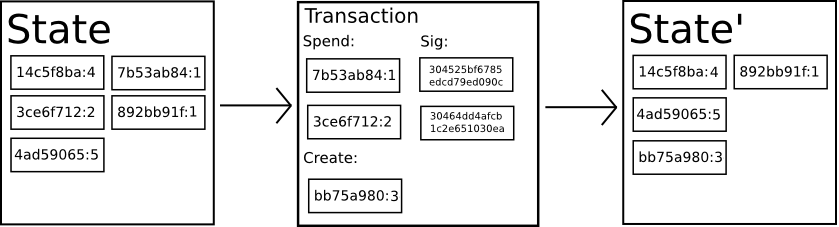
\includegraphics[width=1\linewidth]{Figures/BTC_statetransition_ETH_white_paper}
\decoRule
\caption{Bitcoin Zustandsveränderung durch Transaktion}
\label{fig:BTC_statetransition_ETH_white_paper}
\end{figure}

Die Transaktion aus Abbildung \ref{fig:BTC_statetransition_ETH_white_paper} überweist 1 Bitcoin von der Adresse \code{7b53ab84} und 2 Bitcoin von Adresse \code{3ce6f712} auf die Adresse \code{bb75a980} und überführt somit das Kontobuch in einen neuen Zustand. Möchten mehrere Teilnehmer den Systemzustand durch Transaktionen gleichzeitig anpassen, spielt die Reihenfolge, in der die Transaktionen ausgeführt werden, eine wichtige Rolle. Aus diesem Grund werden Transaktionen in sogenannten Blöcken, in einer festen Reihenfolge, aggregiert. Somit werden nicht einzelne Transaktionen, sondern ganze Blöcke von Transaktionen in die Datenbank geschrieben. Genau wie bei den Transaktionen gibt es auch für Blöcke gewisse Konsensregeln. Sobald ein Block allen Konsensregeln entspricht, ist er bereit in die Datenbank aufgenommen zu werden.
Da sich alle Netzwerkteilnehmer über die Gültigkeit des Blockes einig sind, wird somit die globale Blockchain Datenbank angepasst. Genau wie bei den Transaktionen ist auch die Reihenfolge der Blöcke wichtig. Daher beinhaltet jeder Block den Hash-Wert seines Vorgängers(siehe \ref{fig:blockchain_ETH_white_paper}).

\begin{figure}[H]
\centering
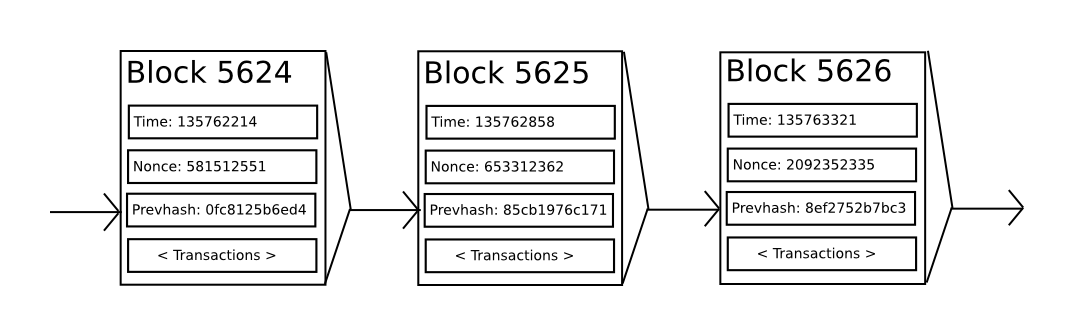
\includegraphics[width=1\linewidth]{Figures/blockchain_ETH_white_paper}
\decoRule
\caption[Kette von Blöcken]{Verkettung von Blöcken.}
\label{fig:blockchain_ETH_white_paper}
\end{figure}

Durch die so erzielte Verkettung der Blöcke wird die Reihenfolge eindeutig festgelegt und es entsteht die sogenannte Blockchain. Am Anfang der Blockchain befindet sich der sogenannte Genesis Block. Auf diesen bauen alle weiteren Blöcke auf. Nachträgliche Änderungen an einem bereits eingefügtem Block sind nicht möglich, da sich dadurch der Blockhash des Blocks verändert und somit an dieser Stelle die Kette ''zerbricht''.

\subsection{Konsensregeln}

Konsenzregeln sind Regeln über die sich alle Teilnehmer des Peer-to-Peer-Netzwerks einig sind. Sie stellen sicher, dass die grundlegenden Eigenschaften der Kryptowährung eingehalten werden. 
\if
Protokollregeln legen die Syntax der ausgetauschten Nachrichten fest. Konsensregeln legen dagegen die Semantik der ausgetauschten Nachrichten fest. 
Konsensregeln sind den Protokollregeln übergeordnet. Dies bedeutet, dass eine laut Protokollregeln korrekt aufgebaute Transaktionsnachricht, dennoch eine ungültige Transaktion enthalten kann, die den Konsensregeln widerspricht.
\fi
Bei Bitcoin gibt es eine ganze Reihe an Konsensregeln. Die wichtigsten sind:
\begin{itemize}
\item Transaktionen dürfen kein Geld aus dem nichts schöpfen, sondern nur bereits existierende Beträge von einer Adresse auf eine andere Adresse überweisen. Die Blockreward-Konsensregel bildet hierzu die einzige Ausnahme. Sie legt fest wie neue Währungseinheiten erschaffen werden.
\item Blockreward: Ein neuer Block muss genau eine Transaktion enthalten, die neue Kryptowährungseinheiten aus dem nichts erschafft. Sowohl die Höhe des Betrags als auch die Anpassung des Betrags über die Zeit ist in den Konsensregeln des Protokolls hart verankert. Bei Bitcoin halbiert sich der Blockreward jedes mal nach einer festgelegten Zeitspanne. Dies stellt sicher, dass es eine feste Obergrenze an Währungseinheiten gibt.
\item Transaktionen, die Geld von Adresse A nach Adresse B überweisen, müssen durch eine Signatur beweisen, dass sie von dem rechtmäßigen Besitzer getätigt werden.
\item Blockgröße: Diese Konsensregel legt die maximale Größe eines Blocks in Megabyte fest. Sie beeinflusst wie viele Transaktionen in einem Block gebündelt werden können. Dies ist wichtig, da sie zusammen mit der Blockzeit-Konsensregel das Wachstum der Blockchain-Datenbank steuert.
\item Blockzeit: Diese legt fest in welchem durchschnittlich Zeitabstand es erlaubt ist einen neuen Block in die Blockhain einzufügen. Bei Bitcoin ist diese Zeit auf 10 Minuten festgelegt.
\item Längste Blockchain-Kette: Teilnehmer des Peer-to-Peer Netzwerks folgen immer der Kette, die am meisten Proof-of-Work beinhaltet und betrachten ''kürzere'' Ketten als ungültig.
\end{itemize}
Die Konsensregeln ermöglichen es, dass jeder Teilnehmer eigenständig lokal seine Version der Blockchain Datenbank verwalten kann, ohne dabei einem anderen Teilnehmer vertrauen zu müssen. Die Konsensregeln stellen somit sicher, dass alle Teilnehmer die gleiche Blockchain Datenbank lokal aufbauen und sich dadurch auf den Systemzustand einigen.

\if Dadurch herrscht Einigkeit darüber welche Transaktionen bereits in die Blockchain aufgenommen wurden und somit als bestätigt gelten. Alle noch nicht in die Blockchain aufgenommen Transaktionen gelten als unbestätigt. \fi

\subsection{Proof-of-Work und Mining}
Bei einer dezentralen Währung wie Bitcoin gibt es keine zentrale Instanz, die eine Anpassung des Systemzustands koordiniert, beziehungsweise autorisiert. Um dieses Problem zu lösen verwendet Bitcoin einen Proof-of-Work Algorithmus. Dieser basiert auf der Idee, dass Teilnehmer des Netzwerks nachweisen müssen, dass sie einen gewissen Aufwand aufgebracht haben, bevor sie einen neuen Block an die Blockchain anhängen dürfen. Um den nächsten gültigen Block zu produzieren, muss der Hashwert des Blocks unter einem dynamisch angepassten Schwierigkeit-Zielwert liegen. Der Schwierigkeit-Zielwert wird durch die Blockzeit Konsensregel so angepasst, dass im gesamten Netzwerk im Durchschnitt alle 10 Minuten ein neuer Bitcoin Block gefunden wird. Bei der Suche nach einem gültigen Block wird nach jeder Berechnung des Hashwerts das \code{nonce}-Feld des Blockheaders erhöht, damit ein neuer Hashwert entsteht. Findet ein Teilnehmer den Blockhash eines den Konsensregeln entsprechenden Blocks, leitet er diesen Block an das Peer-to-Peer Netzwerk weiter und erhält im Gegenzug den Blockreward. Teilnehmer, die unbestätigte\footnote{Alle gültigen Transaktionen, die noch nicht Teil der längsten Blockchain sind, gelten als unbestätigt.} Transaktionen empfangen, diese in Blöcke zusammenfassen und unter Zuhilfenahme des Proof-of-Work Algorithmus in die Blockchain einfügen, werden ''Miner'' genannt. Dieser Name stammt daher, dass bei diesem rechenintensiven Prozess gleichzeitig neue Bitcoins erschaffen werden.

Beim Mining werden die in Tabelle \ref{tab:btc_block_header} aufgeführten Felder des Blockheaders als Eingabe für die kryptographische Hashfunktion SHA256 verwendet\footnote{Um genau zu sein wird der Blockheader bei Bitcoin zweimal mit der SHA 256 Hashfunktion gehasht. Blockhash = SHA256(SHA256(Blockheader))}.
\begin{table}[H]
\centering
\caption{Bitcoin Blockheader}
\label{tab:btc_block_header}
\begin{tabular}{|l|p{4,3cm}|p{4,3cm}|l|}
\hline
\textbf{Feld}  & \textbf{Verwendungszweck}                         & \textbf{Aktualisiert falls...}                                          & \textbf{Bytes} \\ \hline
version        & Block Versionsnumber                             & man die Software aktualisiert und diese eine neue Version spezifiziert. & 4              \\ \hline
hashPrevBlock  & 256-bit Hash des vorherigen Blockheaders          & ein neuer gültiger Block empfangen wird.                                & 32             \\ \hline
hashMerkleRoot & 256-bit Hash aller Transaktionen des Blocks       & eine neue Transaktion akzeptiert wird.                                  & 32             \\ \hline
time           & Aktueller Zeitstemple in Sekunden seit 1970-01-01 & Alle paar Sekunden...                                                   & 4              \\ \hline
bits           & Aktuelles Schwierigkeitsziel                      & wenn das Schwierigkeitsziel angepasst wird.                             & 4              \\ \hline
nonce          & 32-bit Nummer (von 0 aus erhöht)                  & der Hash ausprobiert wurde. (nonce+1)                                   & 4              \\ \hline
\end{tabular}
\end{table}
Die Transaktionen des Blocks gehen nicht direkt, nur durch den sogenannten Merkel Tree Hash\footnote{Der genaue Aufbau des Merkel Trees und dessen Vorteile sind in \cite{bitcoin_white_paper} genauer beschrieben.} in den Blockhash mit ein. Das \code{nonce}-Feld des Blockheaders wird nach jedem Hashversuch um den Wert 1 erhöht. Dadurch wird die Ausgabe der Hashfunktion kontinuierlich verändert.

Die Sicherheit des Bitcoin Netzwerkes und die Unmanipulierbarkeit der Blockchain ergeben sich aus der im Protokoll verankerten Spieltheorie. Die Spieltheorie macht es für einen Miner profitabler sich an die Spielregeln des Protokolls zu halten als zu versuchen das Netzwerk zu betrügen. Versucht ein Miner einen Block zu produzieren, der den Konsensregeln widerspricht, wird dieser vom Netzwerk verworfen. Somit hält kein anderer Netzwerkteilnehmer den vom Miner an sich selbst ausgeschütteten Blockreward für gültig. Da der Miner aber Ausgaben in Form von Hardwareabnutzung und Stromkosten zu bezahlen hat, schafft dies einen Anreiz sich den Konsensregeln zu unterwerfen. Solange 51 Prozent der Miner sich den Konsensregeln unterwerfen, formen diese auf Dauer die längste Blockchain. 

Die beim Mining anfallenden Stromkosten machen es außerdem sehr Teuer die Geschichte der Blockchain neu zu schreiben. \todo{entweder im Proof of stake kapitel verwenden oder rausnehmen.}

Das Mining ist ein sich selbst regulierendes System bei dem die Anzahl Miner\footnote{Genauer gesagt nicht die Anzahl Miner, sondern die von den Minern erbrachte Rechenleistung.} sich mit dem Wert der Kryptowährung anpasst. Steigt der Preis pro Bitcoin, kommen neue Miner zum Netzwerk hinzu und machen das Netzwerk sicherer. Ein sinkender Preis hat zur Folge, dass der Blockreward nicht mehr für die Bezahlung der Strom und Hardwarekosten ausreicht. Dies hat zur Folge, dass die Anzahl an Miner abnimmt. Somit sinkt auch die Sicherheit des Netzwerks.\todo{ein sich selbst regulierendes System: Falsch, es gibt keine Rückkopplung. Nochmal drüber nachdenken was ich hier wirklich sagen will.} 
\section{Konzept}

Die folgenden Schritte beschreiben den Finanzfluss zwischen den Teilnehmern und der Anwendung sowie die Gewinnerauswahl durch den in der Zukunft liegenden Blockchain-Status. Der Ablauf ist allgemein gehalten und kann nicht nur mit Bitcoin, sondern auch mit anderen Kryptowährungen, die auf einer Proof-of-Work Blockchain basieren, umgesetzt werden. Betrachtet wird ein Spiel mit $N \in \{2,5,10\}$ Teilnehmern, bei dem jeder Teilnehmer einen Einsatz von $X$ Währungseinheiten zur Teilname zahlen muss. 

\begin{enumerate}
\item Im ersten Schritt eröffnet die Anwendung ein neues Spiel in dem es $N$ freie Plätze und einen leeren Geldtopf gibt.
\item Sobald ein Spieler am Spiel teilnehmen möchte, generiert die Anwendung eine neue Empfangsadresse\footnote{Man könnte auch allen Spieler die gleiche Einzahlungsadresse anzeigen. (siehe \ref{sssec:Auszahlungstransaktion})} und zeigt diese dem Spieler an.
\item Der Spieler verwendet die Wallet Software seiner Wahl um eine Transaktion zu erstellen, die den Einsatz an die angezeigte Empfangsadresse überweist. Die Wallet Software signiert die Transaktion und leitet sie über die mit ihr verbundenen Nachbarn an das Peer-to-Peer Netzwerk weiter.
\item Ein Miner empfängt die Transaktion und nimmt sie in den nächsten Block auf.
\item Der Miner findet den zu seinem Block passenden Proof-of-Work-Hash und schickt den Block an das Netzwerk.
\item Die Applikation empfängt den Block und merkt, dass im Block eine Transaktion auf die in Schritt 2 generierte Empfangsadresse enthalten ist. Die Applikation prüft die Höhe des Transaktionsbetrag und leitet anschließend die vom Spieler kontrollierte Auszahlungsadresse aus der Transaktion ab. 
\item  Die restlichen $N-1$ Teilnehmer überweisen ebenfalls den geforderten Betrag auf die ihnen angezeigte Empfangsadresse.
\item  Sobald die letzte Transaktion in einen validen Block aufgenommen wurde, zählt die Reihenfolge in der die Transaktionen in der Blockchain stehen. Die Reihenfolge steht somit fest und kann nicht mehr nachträglich verändert werden. Der Geldtopf ist nun mit einem Betrag von $N*X$ Krytowährungseinheiten gefüllt und wird geschlossen. Der Block nach dem Block, in dem die letzte Einzahlungstransaktion eingegangen ist, wird zur Gewinnerauswahl genutzt. Die Anwendung merkt sich die Blocknummer dieses Blocks.
%\item Die Anwendung signiert nun die Reihenfolge der Teilnehmer und deren Auszahlungsadressen und schreibt die resultierende Signatur mit einer Transaktion in die Blockchain.
\item Die Anwendung und die Teilnehmer warten darauf, dass der nächste Block von einem Miner gefunden wird. Alle Miner des Peer-to-Peer Netzwerks versuchen schnellstmöglich einen passenden Blockhash zu finden um den Blockreward zu erhalten. Ein Miner gewinnt dieses Rennen und teilt dem Netzwerk den neu gefundenen Block mit.
\item Die Anwendung empfängt den nächsten Block und ermittelt durch diesen den Gewinner. Die Berechnung erfolgt auf Basis der letzten Dezimalstelle $d_{last}$ des Blockhashs\footnote{Man kann an dieser Stelle auch den gesamten Blockhash als Grundlage der Gewinnerauswahl nehmen. Die daraus resultierenden Vor- und Nachteile werden in Abschnitt \ref{btc_gewinnerauswahl} erörtert.}. Durch die Berechnung von $d_{last}$  modulo $N$ resultiert eine Zahl $G \in \{0,...,N-1\}$, die den Gewinner festlegt. Der Spieler, der die $G+1$te Einzahltransaktion gesendet hat, gewinnt den Geldtopf.
\item Die Anwendung erstellt eine Transaktion, die alle $N*X$ Krytowährungseinheiten des Geldtopfs an die Auszahlungsadresse des Gewinners überweist, und sendet diese an das Netzwerk.
\item Die Wallet Software des Gewinners, empfängt die Transaktion und informiert ihn darüber, dass er den gesamten Betrag des Topfes erhalten hat.
\end{enumerate}

%%%%%%%%%%%%%%%%%%%%
% Bitcoin Beispiel %
%%%%%%%%%%%%%%%%%%%%
\vspace{1cm}
Im folgenden Beispiel wird einen Topf mit 5 Teilnehmern, die Kryptowährung Bitcoin und einen Einzahlungsbetrag von 0,1 Bitcoin betrachtet. Dieses Beispiel verdeutlicht sowohl die Interaktion der verschiedenen Teilnehmer des Peer-to-Peer Netzwerks, als auch die Veränderung des Status der Blockchain.

\vspace{1cm}
\begin{minipage}{0.55\textwidth}
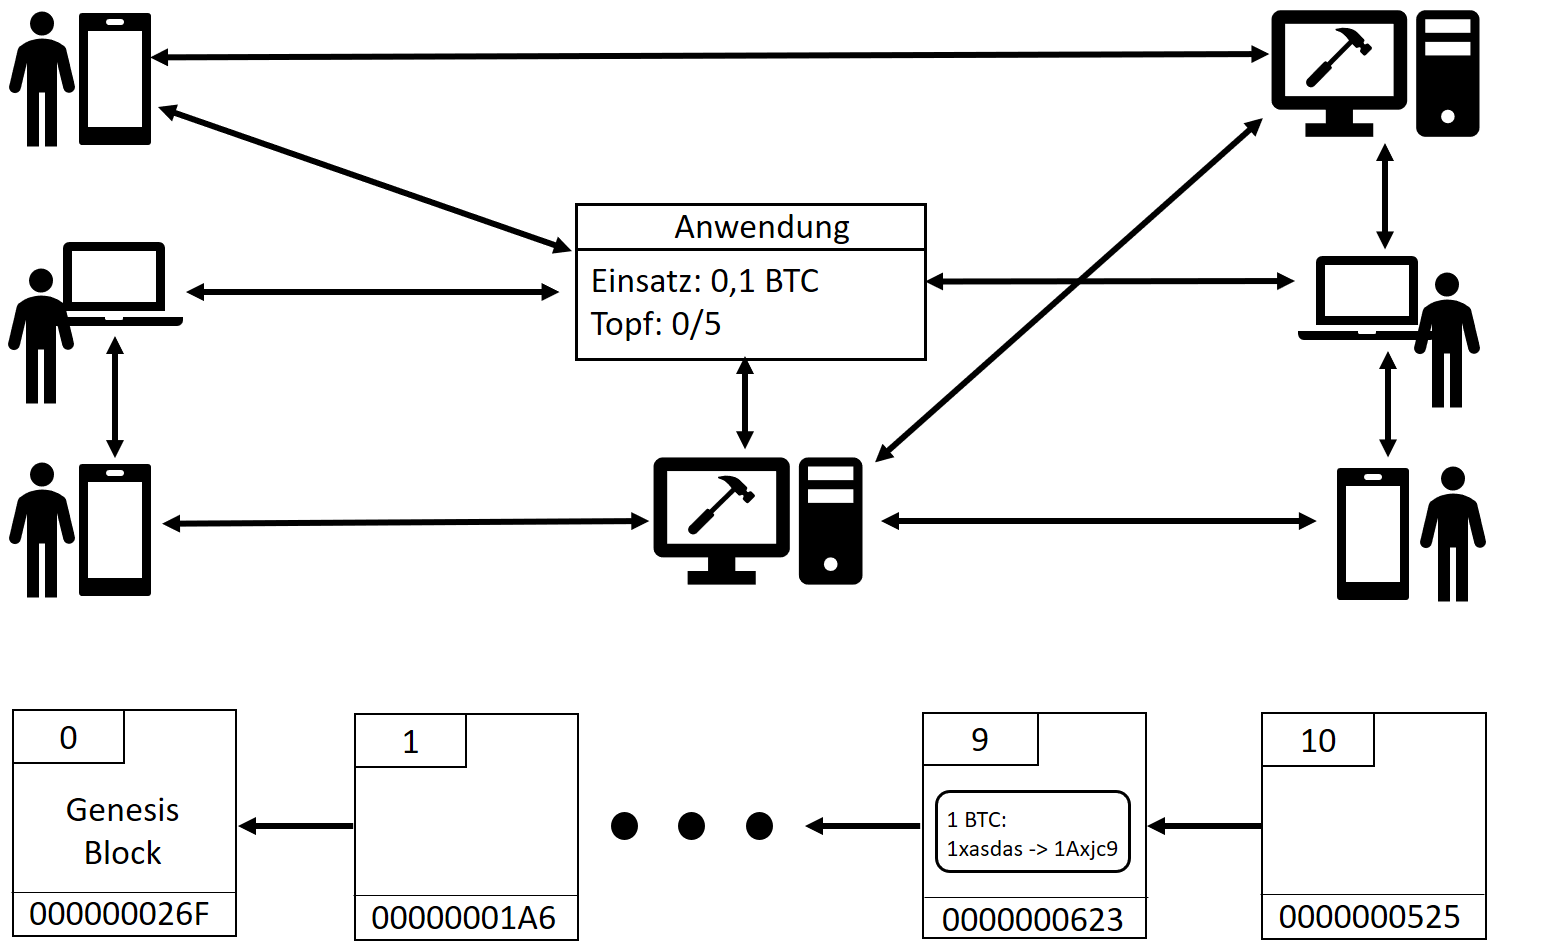
\includegraphics[width=\textwidth]{Figures/konzept_btc/konzept1}
\centering
\decoRule
\captionof{figure}{Schritt 1}
\label{fig:konzept1}
\end{minipage}
\begin{minipage}{0.45\textwidth}
Diese Abbildung zeigt das Peer-To-Peer Netzwerk. Die 5 potentiellen Teilnehmer sind durch Notebooks und Smartphones dargestellt. Außerdem sind 2 Miner und die Glücksspielanwendung teil des Peer-To-Peer Netzwerks. Der aktuelle Status der Blockchain, die jeder Teilnehmer des Netzwerks lokal speichert, ist unterhalb des Netzwerkes dargestellt.
\end{minipage}

\vspace{1cm}
\begin{minipage}{0.55\textwidth}
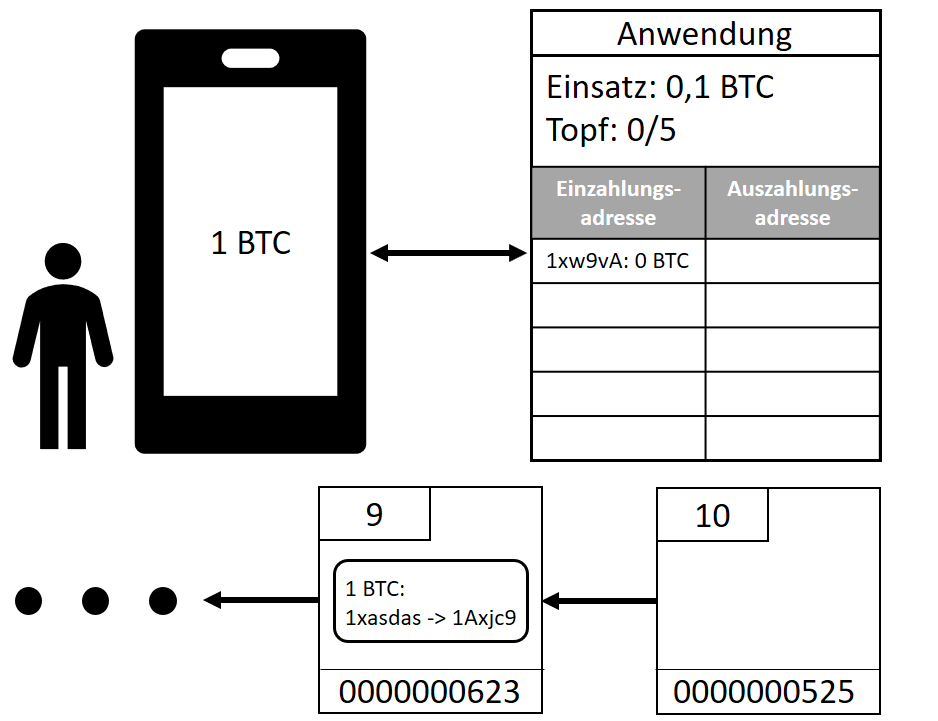
\includegraphics[width=\textwidth]{Figures/konzept_btc/konzept2}
\centering
\decoRule
\captionof{figure}{Schritt 2}
\label{fig:konzept2}
\end{minipage}
\begin{minipage}{0.45\textwidth}
Die Bitcoin Client Software der Glücksspielanwendung generiert eine neue Bitcoinadresse und speichert den dazugehörigen privaten Schlüssel in der Wallet. Sobald Bitcoins auf dieser Adresse empfangen werden, können sie nur durch den Besitz des privaten Schlüssels weiter transferiert werden.
Die Anwendung zeigt dem Benutzer eine frisch generierte Empfangsadresse über die Benutzeroberfläche an. Der Zustand der Blockchain verändert sich nicht.
\end{minipage}

\vspace{1cm}
\begin{minipage}{0.55\textwidth}
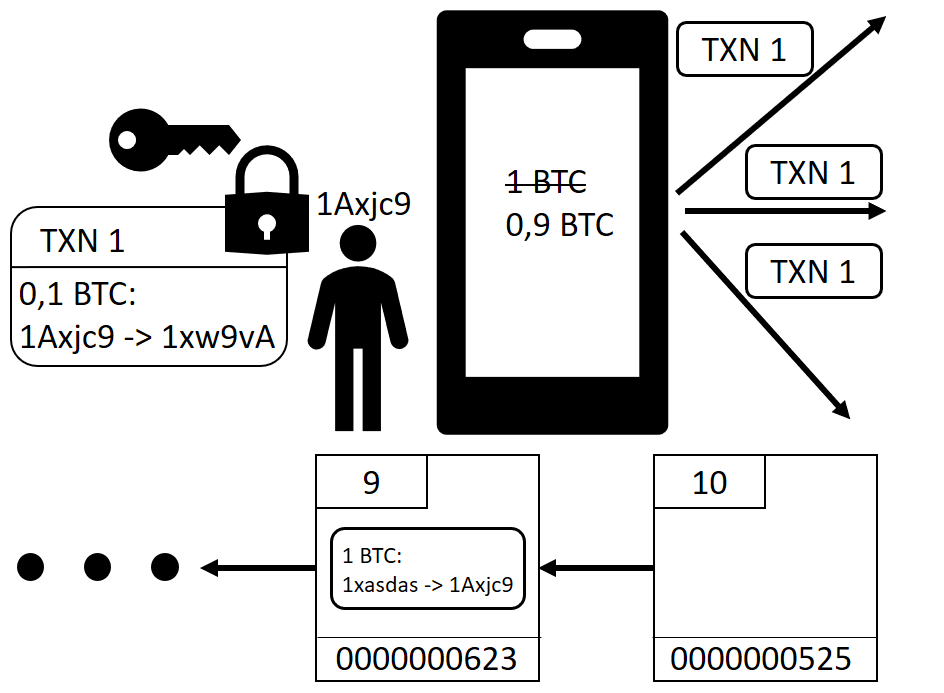
\includegraphics[width=\textwidth]{Figures/konzept_btc/konzept3}
\centering
\decoRule
\captionof{figure}{Schritt 3}
\label{fig:konzept3}
\end{minipage}
\begin{minipage}{0.45\textwidth}
Nun zahlt der Spieler mit Hilfe seiner Bitcoin Wallet Software in den Geldtopf ein. Dazu erstellt er eine Transaktion, die Bitcoin von seiner Adresse auf die generierte Adresse der Glücksspielanwendung transferiert. Durch die Signierung mit seinem privaten Schlüssel autorisiert er die Überweisung. Anschließend schickt er die Transaktion seinen Nachbarn.
\end{minipage}

\vspace{1cm}
\begin{minipage}{0.55\textwidth}
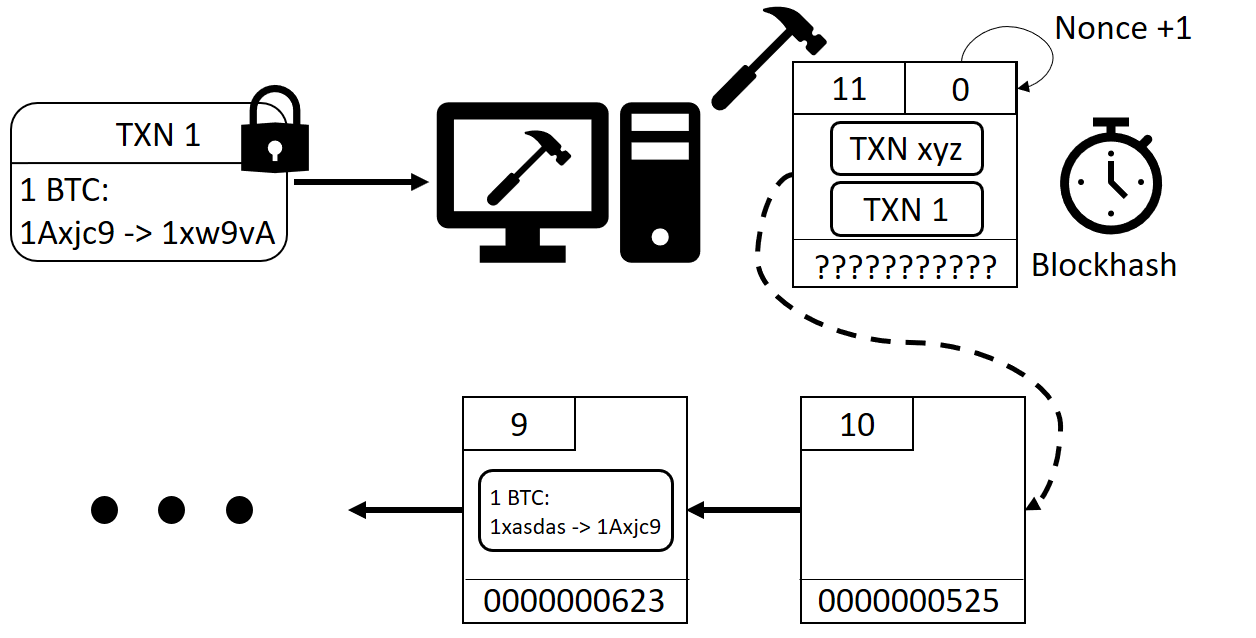
\includegraphics[width=\textwidth]{Figures/konzept_btc/konzept4}
\centering
\decoRule
\captionof{figure}{Schritt 4}
\label{fig:konzept4}
\end{minipage}
\begin{minipage}{0.45\textwidth}
Sobald die Transaktion TXN 1 einen Miner erreicht, prüft dieser, ob die Transaktion in Einklang mit den Konsensregeln ist. In diesem Beispiel existiert in Block 9 eine Transaktion von einem Bitcoin auf die Adresse des Teilnehmers. Unter der Annahme, dass dieser Bitcoin nicht in Block 10 weiter überwiesen wurde, befindet sich auf der Adresse des Teilnehmers somit ein Bitcoin. Außerdem prüft der Miner ob die Signatur der Transaktion gültig ist. Da die Transaktion valide ist, fügt er sie dem aktuell zu generierenden Block Nummer 11 hinzu. 
\end{minipage}


\vspace{1cm}
\begin{minipage}{0.55\textwidth}
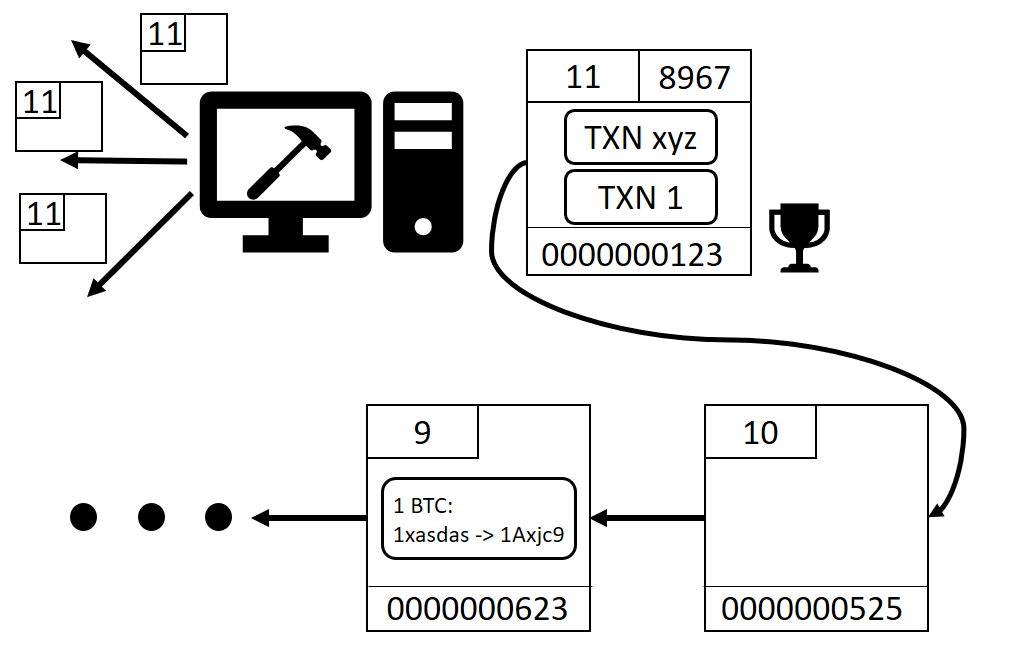
\includegraphics[width=\textwidth]{Figures/konzept_btc/konzept5}
\centering
\decoRule
\captionof{figure}{Schritt 5}
\label{fig:konzept5}
\end{minipage}
\begin{minipage}{0.45\textwidth}
Der Miner berechnet nun mithilfe der Hashfunktion den Hash des Blocks. Falls der Blockhash-Wert den durch die Konsensregeln dynamischen angepassten Schwierigkeits-Wert unterschreitet, gilt der Block als valide. Überschreitet der Blockhash den Wert, erhöht der Miner den Nonce-Wert des Blocks und berechnet den Blockhash erneut. Diesen Prozess wiederholt er solange bis er entweder einen gültigen Blockhash findet oder einen gültigen Block Nummer 11 von einem anderen Netzwerkteilnehmer empfängt.
In diesem Beispiel findet der Miner einen gültigen Blockhash, leitet den Block ans Netzwerk weiter und wird dadurch mit neu erschaffenen Bitcoin für seinen Rechenaufwand belohnt.
\end{minipage}

\vspace{1cm}
\begin{minipage}{0.55\textwidth}
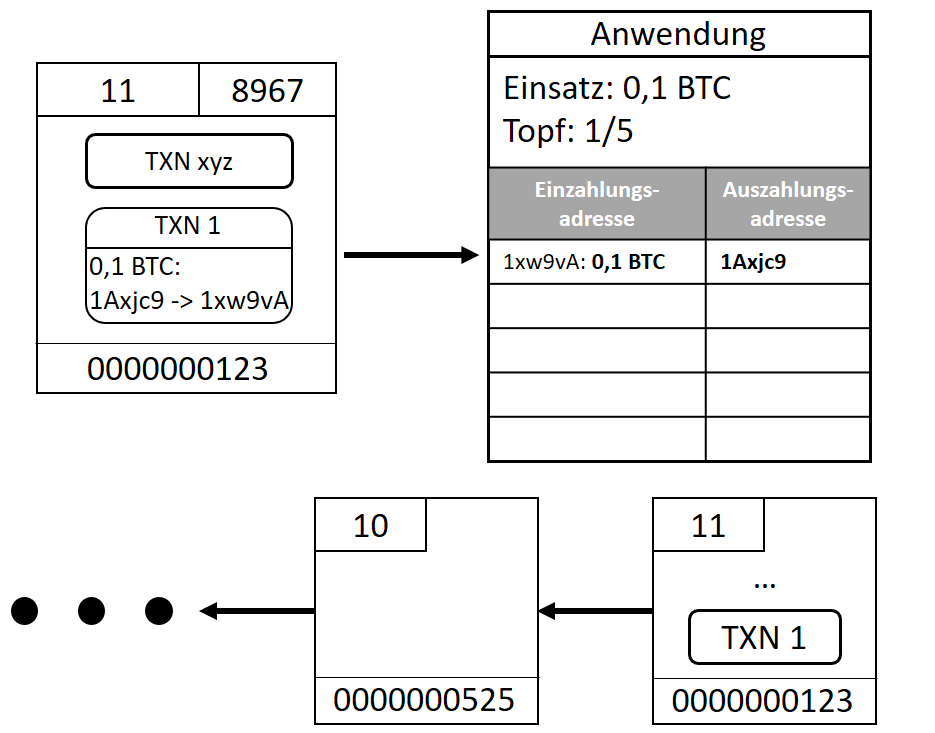
\includegraphics[width=\textwidth]{Figures/konzept_btc/konzept6}
\centering
\decoRule
\captionof{figure}{Schritt 6}
\label{fig:konzept6}
\end{minipage}
\begin{minipage}{0.45\textwidth}
Die Glücksspielanwendung empfängt den Block Nummer 11 und überprüft ob er im Einklang mit den Konsensregeln ist. Dies ist der Fall. Somit wird die lokale Blockchain Datenbank um einen Block erweitert. Die Glücksspielanwendung hat somit den Einsatz des ersten Spielers erhalten. Aus der Einzahlungstransaktion des Spielers leitet die Anwendung die Auszahlungsadresse \textbf{1Axjc9} des Spielers ab. 
\end{minipage}

\vspace{1cm}
\begin{minipage}{0.55\textwidth}
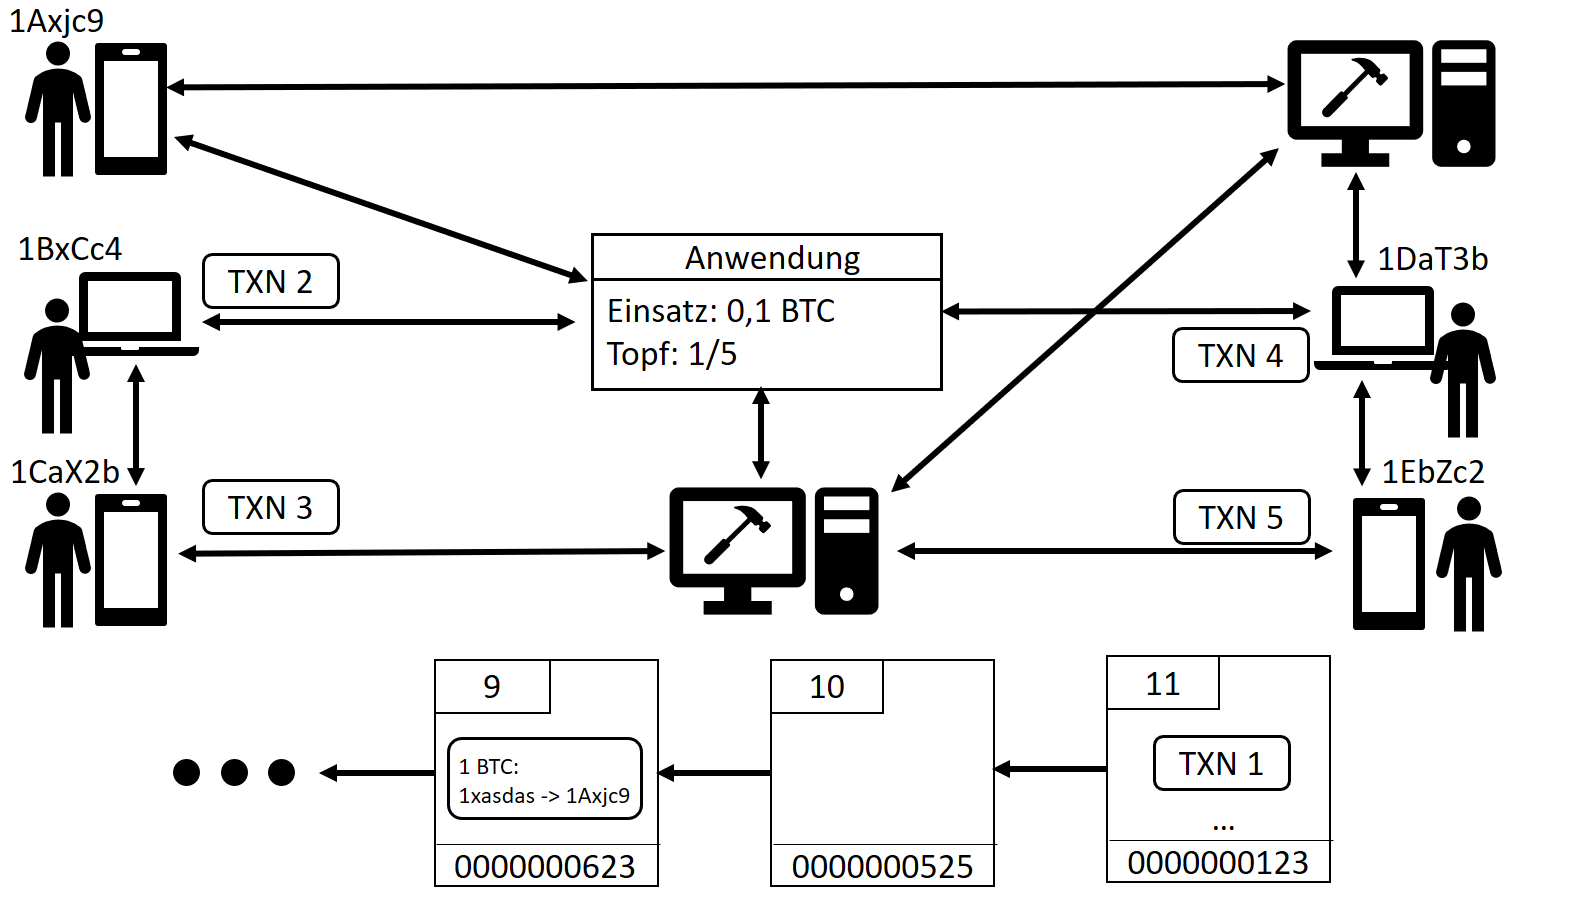
\includegraphics[width=\textwidth]{Figures/konzept_btc/konzept7}
\centering
\decoRule
\captionof{figure}{Schritt 7}
\label{fig:konzept7}
\end{minipage}
\begin{minipage}{0.45\textwidth}
Die restlichen Spieler senden ihre signierten 0,1 Bitcoin Transaktionen ins Peer-to-Peer Netzwerk. Diese sind in Abbildung 7 durch die Transaktionen TXN 2 bis 5 dargestellt.
\end{minipage}

\vspace{1cm}
\begin{minipage}{0.55\textwidth}
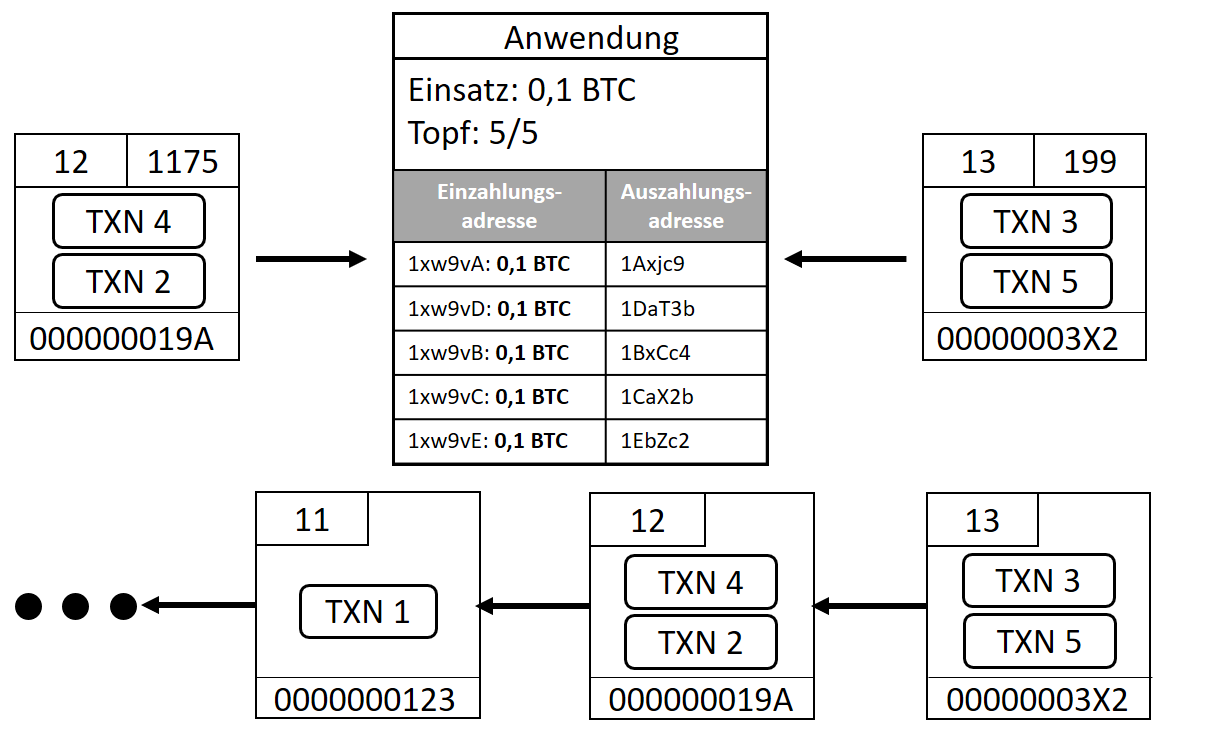
\includegraphics[width=\textwidth]{Figures/konzept_btc/konzept8}
\centering
\decoRule
\captionof{figure}{Schritt 8}
\label{fig:konzept8}
\end{minipage}
\begin{minipage}{0.45\textwidth}
Beliebige Miner fügen die Transaktionen in ihre Blöcke ein. Sobald die Glücksspielanwendung die Blöcke empfängt, prüft sie diese gegen die Konsensregeln und fügt sie in die lokale Blockchain ein.
Die Applikation merkt nun, dass alle Spieler bezahlt haben und schließt den Geldtopf. Dabei merkt sie sich die Nummer des Blocks in der die letzte Einzahlungstransaktion vorhanden ist. Der darauffolgende Block mit Nummer 14 wird für die Ziehung des Gewinners verwendet.
\end{minipage}

\vspace{1cm}
\begin{minipage}{0.55\textwidth}
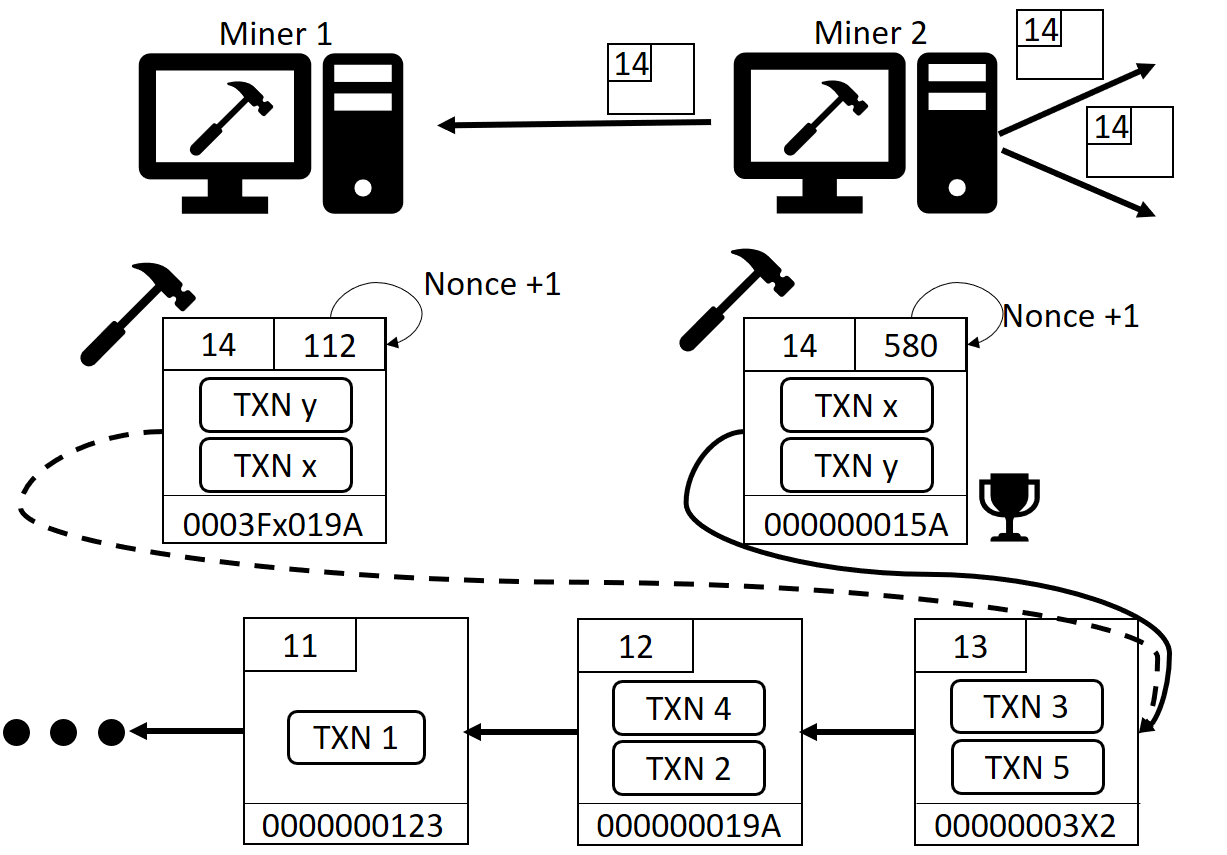
\includegraphics[width=\textwidth]{Figures/konzept_btc/konzept9}
\centering
\decoRule
\captionof{figure}{Schritt 9}
\label{fig:konzept9}
\end{minipage}
\begin{minipage}{0.45\textwidth}
Alle Miner des Netzwerkes versuchen nun gleichzeitig so schnell wie möglich den nächsten Block zu finden. Da sie dazu eine kryptographische Hashfunktion benutzen bei der die Ausgabe ein unkontrollierbarer zufälliger Wert ist, hat keiner der Miner einen direkten Einfluss auf den resultierenden Blockhash. In diesem Beispiel findet Miner 2 einen gültigen Blockhash vor Miner 1. Miner 2 leitet seinen gültigen Block Nummer 14 so schnell wie möglich an das Netzwerk weiter und erhält den Blockreward als Belohnung. Miner 1 geht leer aus.
\end{minipage}

\vspace{1cm}
\begin{minipage}{0.55\textwidth}
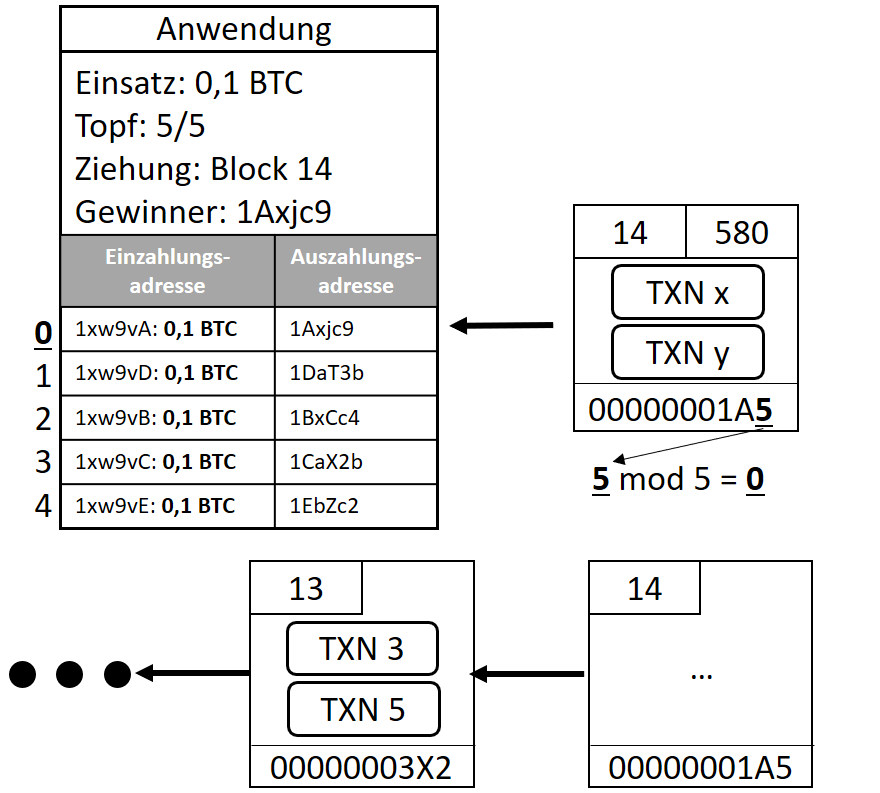
\includegraphics[width=\textwidth]{Figures/konzept_btc/konzept10}
\centering
\decoRule
\captionof{figure}{Schritt 10}
\label{fig:konzept10}
\end{minipage}
\begin{minipage}{0.45\textwidth}
Die Anwendung empfängt Block 14 und prüft ihn gegen die Konsensregeln. Der Block ist valide. Daher verwendet die Anwendung den im Block enthaltenen Blockhash um den Gewinner des Geldtopfes zu ermitteln. Statt des gesamten Blockhashs verwendet die Anwendung nur die letzte Ziffer des Blockhashs zur Gewinnerauswahl. Dies hat den Vorteil, dass die Teilnehmer die Korrektheit der Gewinnerauswahl leichter eigenständig nachprüfen können.
Da die letzte numerische Stelle des Blockhashs 10 verschiedene Werte annehmen kann, ordnet die Anwendung jedem der 5 Teilnehmer mittels der Modulo 5 Funktion zwei Gewinnzahlen zu.
\end{minipage}

\vspace{1cm}
Dadurch ergibt sich die Verteilung der Gewinnzahlen folgendermaßen:
\begin{itemize}
\item Spieler 1 mit Adresse 1xw9vA gewinnt bei 0 und 5,
\item Spieler 2 mit Adresse 1xw9vD gewinnt bei 1 und 6,
\item Spieler 3 mit Adresse 1xw9vB gewinnt bei 2 und 7,
\item Spieler 4 mit Adresse 1xw9vC gewinnt bei 3 und 8,
\item Spieler 5 mit Adresse 1xw9vE gewinnt bei 4 und 9.
\end{itemize}
Jeder Teilnehmer besitzt nun eine Gewinnwahrscheinlichkeit von 1/5. Block Nummer 14 hat den Blockhash \textbf{00000001A5}\footnote{In der Praxis ist jeder Blockhash genau 64 Zeichen lang (Hexadezimalsystem), da Bitcoin die SHA-256 Hashfunktion verwendet. Aufgrund der Länge ist es praktisch unmöglich, dass der Blockhash ausschließlich aus Buchstaben besteht.}. Die zur Gewinnerauswahl benutze Ziffer ist somit die 5. Da 5 modulo 5 den Wert 0 ergibt, gewinnt Spieler 1 mit der Adresse \textbf{1xw9vA}.

\vspace{1cm}
\begin{minipage}{0.55\textwidth}
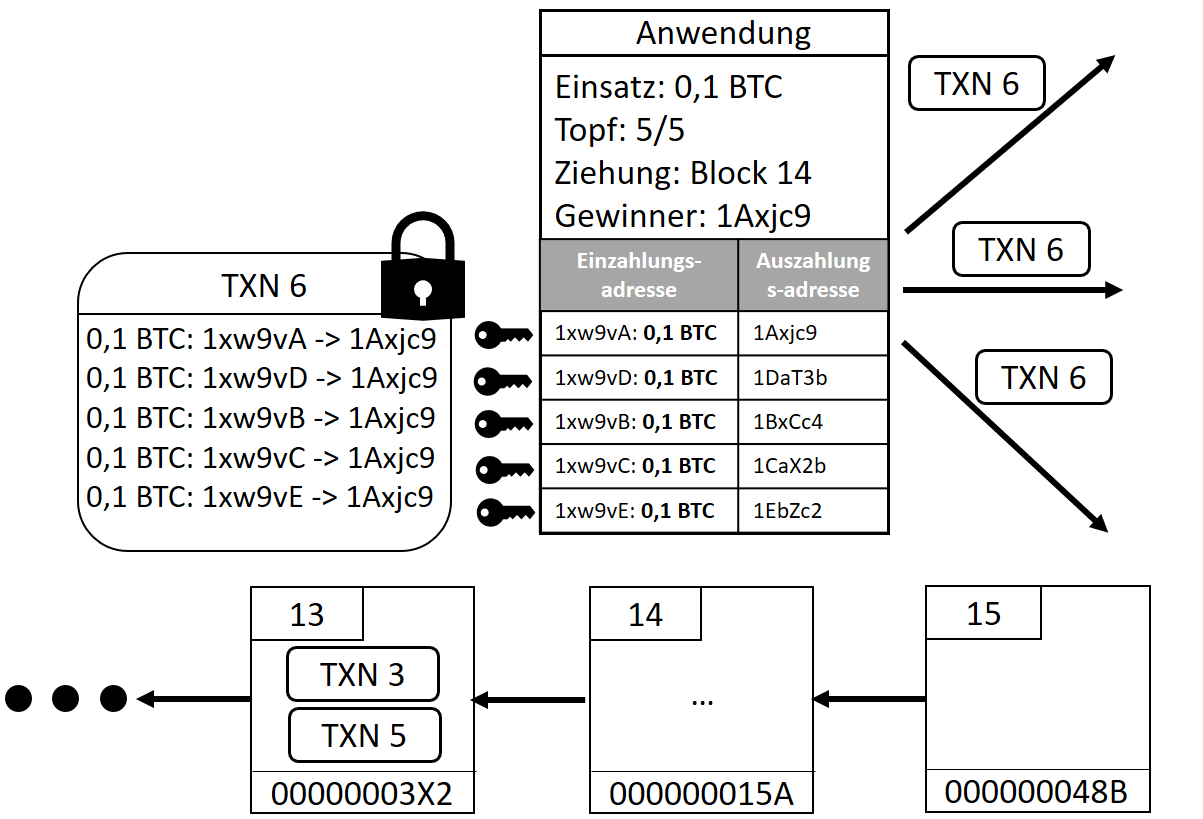
\includegraphics[width=\textwidth]{Figures/konzept_btc/konzept11}
\centering
\decoRule
\captionof{figure}{Schritt 11}
\label{fig:konzept11}
\end{minipage}
\begin{minipage}{0.45\textwidth}
Die Anwendung erstellt nun eine Transaktion die alle Spieleinsätze an die Auszahlungsadresse \textbf{1Axjc9} von Spieler 1 überweist. Um die Transaktion zu signieren verwendet die Anwendung die, zu den 5 Einzahlungsadressen passenden, privaten Schüssel. Anschließend leitet die Anwendung die Transaktion an das Peer-to-Peer Netzwerk weiter.
\end{minipage}

\vspace{1cm}
\begin{minipage}{0.55\textwidth}
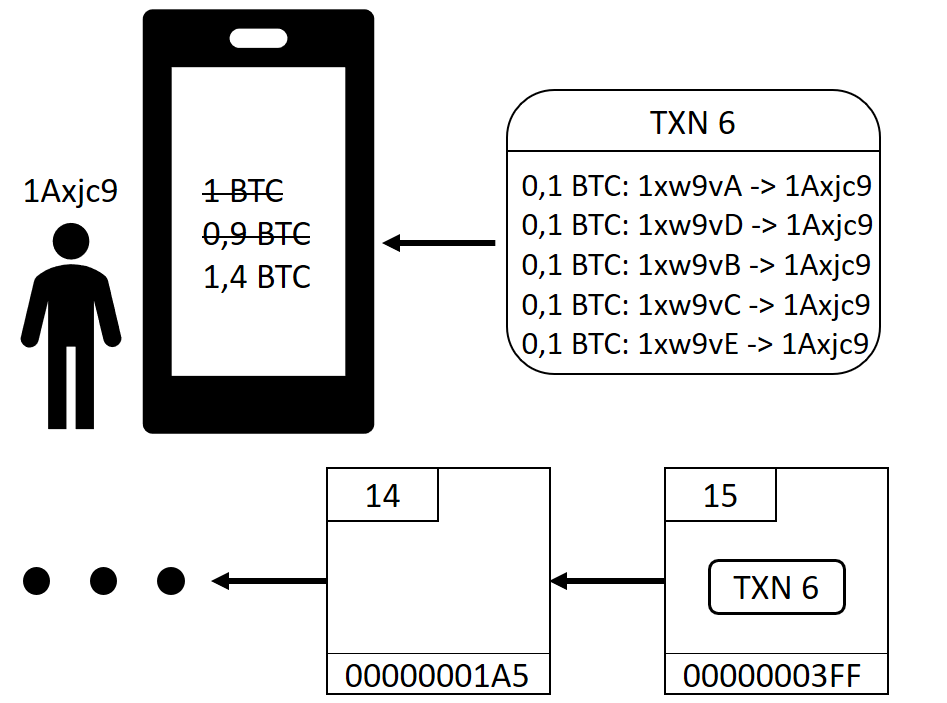
\includegraphics[width=\textwidth]{Figures/konzept_btc/konzept12}
\centering
\decoRule
\captionof{figure}{Schritt 12}
\label{fig:konzept12}
\end{minipage}
\begin{minipage}{0.45\textwidth}
Das Smartphone von Spieler 1 empfängt die Transaktion gegebenenfalls noch bevor sie von einem Miner in einen validen Block aufgenommen wurde. Die Wallet Software zeigt die Transaktion erst als unbestätigt an. Sobald sie durch die Aufnahme in Block 15 bestätigt wurde, gilt sie für die Wallet Software als bestätigt.
\end{minipage} 
\section{Umsetzung}

\subsection{Interaktion mit dem Bitcoin Netzwerk}

Möchte man mit dem Bitcoin Netzwerk kommunizieren, benötigt man einen Client, der das Bitcoin Protokoll implementiert. Dieser interagiert mit dem Peer-to-Peer Netzwerk und wird dadurch zu einem Netzwerk-Knoten. Man unterscheidet zwischen sogenannten \textit{Full-Nodes} und \textit{Light-Nodes}.
\subsubsection{Full-Node}
Knoten die eigenständig alle Transaktionen und Blöcke auf Gültigkeit mit Hilfe der Konsensregeln prüfen, nennt man Full-Node. Diese Knoten speichern die gesamte Blockchain und bilden das Rückgrat des Netzwerks.
Full-Nodes stellen in der Regel eine RPC Schnittstelle zur Verfügung. Diese Schnittstelle bietet die Möglichkeit von einer beliebigen Programmiersprache aus mit dem Full-Node zu interagieren.
Abbildung \ref{fig:btc_core_full_node_architecture} zeigt, dass man über die RPC Schnittstelle auf die gespeicherten Daten des Nodes (Blöcke, Blockheader und Adressen) als auch auf die Wallet zugreifen kann.

\begin{figure}[H]
\centering
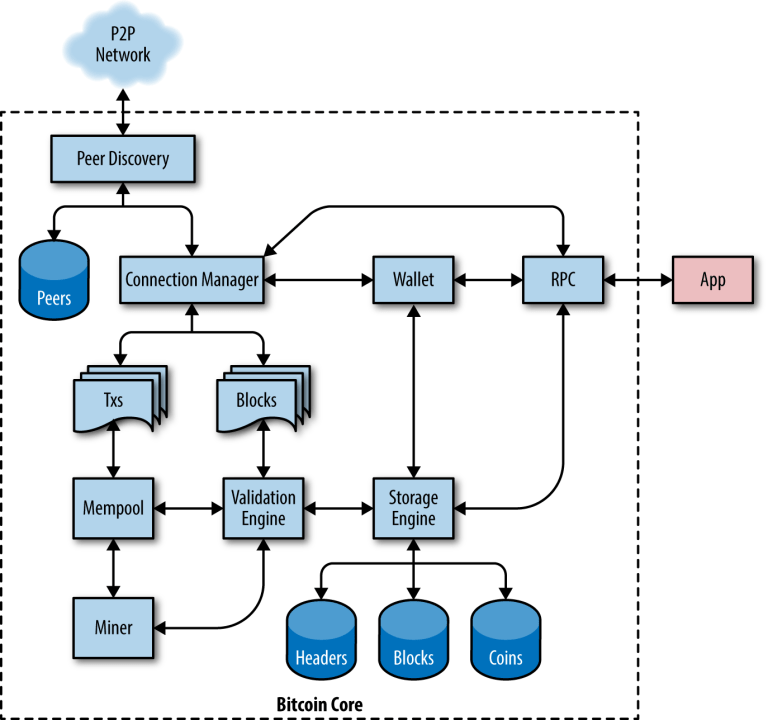
\includegraphics[width=1\linewidth]{Figures/btc_core_full_node_architecture}
\decoRule
\caption{Bitcoin Core: Full-Node Aufbau \cite{mastering_bitcoin}}
\label{fig:btc_core_full_node_architecture}
\end{figure}
Abbildung \ref{fig:btc_core_full_node_architecture} zeigt außerdem: 
\begin{itemize}
\item Peer Discovery, Peer Datenbank und Connection Manager: Diese kümmern sich um die Kommunikation mit dem Peer-to-Peer Netzwerk.
\item Mempool: Im sogenannten Mempool werden empfangene, unbestätigte Transaktionen im Speicher gehalten.
\item Validation Engine: Diese validiert, ob die empfangenen Blöcke und deren Transaktionen die Konsensregeln einhalten. Falls ja werden die somit bestätigten Transaktionen aus dem Mempool gelöscht und der Block wird an die StorageEngine zur Abspeicherung in der Blockchain Datenbank weitergereicht.
\item Miner: Die Bitcoin Full-Node Software enthält einen CPU Miner mit der man mithilfe des Proof-of-Work Algorithmus nach neuen Blöcken suchen kann. Bitcoin Mining ist heutzutage allerdings nur noch mit sogenannten ASICs profitabel. ASIC steht für \textbf{A}pplication-\textbf{S}pecific \textbf{I}ntegrated \textbf{C}ircuit. Es handelt sich um Hardware, die auf eine möglichst performante Berechnung der SHA256 Hashfunktion spezialisiert ist.
\end{itemize}


\subsubsection{Light-Node}
Light-Nodes speichern nicht die gesamte Blockchain, sonder in der Regel nur die Blockheader der Blöcke der Blockchain. Beim Mining gehen nur die Daten des Blockheaders in den Blockhash ein (siehe \ref{tab:btc_block_header}). Der Node empfängt Blockheader, prüft ihre Gültigkeit und fügt sie gegebenenfalls in die Headerkette ein. Der Node kann somit eigenständig, d.h. ohne seinen Nachbarn vertrauen zu müssen, die längste Proof-of-Work Kette bilden. Da diese Kette nur aus Headern besteht und keine Transaktionen enthält, kann der Light-Node empfangene Transaktionen nicht eigenständig auf ihre Gültigkeit prüfen. Light-Nodes verwenden das in \cite{bitcoin_white_paper} beschriebene \textbf{S}implified \textbf{P}ayment \textbf{V}erification Verfahren zur Prüfung von Transaktionen. Light-Nodes werden daher oft auch \textit{SPV-Client} genannt. Ein \textbf{SPV}-Client prüft die Gültigkeit einer Transaktion, indem er sie an der richtigen Stelle der Headerkette einordnet und dann den passenden Merkel-Branch von einem Full-Node anfragt. Durch diese Zusätzlichen Daten kann er nun wie in Abbildung \ref{fig:spv_chain} gezeigt nachprüfen, ob der Hash der Transaktion wirklich in den Wurzelknoten des Merkel-Trees mit eingegangen ist.

\begin{figure}[H]
\centering
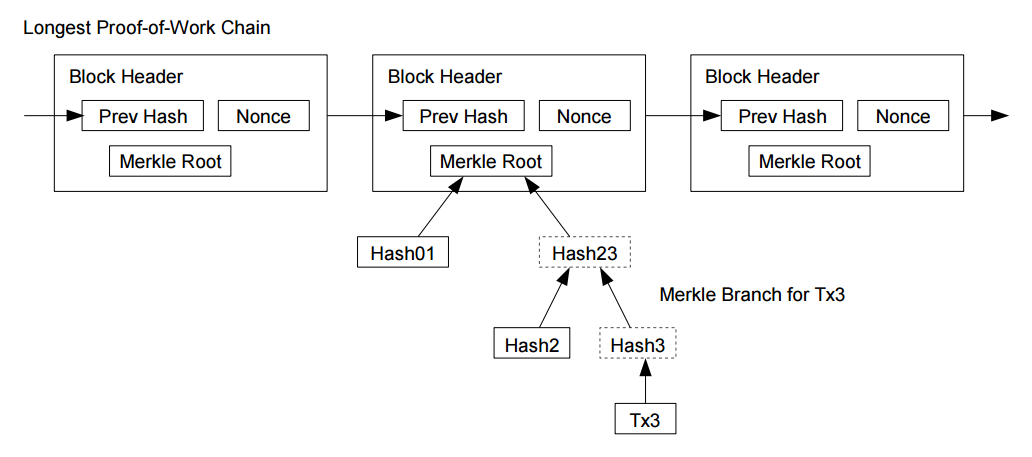
\includegraphics[width=1\linewidth]{Figures/umsetzung_btc/spv_chain}
\decoRule
\caption{Blockheader Kette \cite{ethereum_white_paper}}
\label{fig:spv_chain}
\end{figure}

Für den Bitcoin Teil dieser Ausarbeitung ist die Integration mit dem Peer-to-Peer Netzwerk mit Hilfe der in Java geschriebenen BitcoinJ \cite{bitcoinj} Bibliothek umgesetzt. Diese ermöglicht die Interaktion mit dem Netzwerk als SPV-Client.

\subsection{Überblick}

Abbildung \ref{fig:anwendung_aufbau} skizziert die Komponenten der Glücksspielanwendung und wie diese mit ihrer Umgebung kommunizieren. Es gibt zum einen den Server auf dem die Glücksspielanwendung läuft, die Spieler und das Bitcoin Netzwerk.

\begin{figure}[H]
\centering
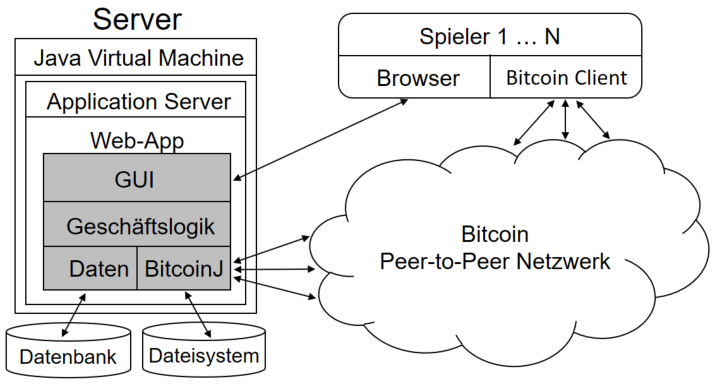
\includegraphics[width=1\linewidth]{Figures/umsetzung_btc/anwendung_aufbau}
\decoRule
\caption{Glücksspielanwendung Aufbau und Interaktion}
\label{fig:anwendung_aufbau}
\end{figure}

\subsubsection{Glücksspielanwedung}
\begin{itemize}
\item Server: Die Glücksspielanwendung läuft auf einem Server, der über eine Java Virtual Machine (JVM) Laufzeitumgebung verfügt, eine MySQL Datenbank und ein gewöhnliches Dateisystem besitzt.
\item Java Virtual Machine (JVM): Innerhalb der JVM läuft ein sogenannter Application Server, der eine Webanwendung nach außen bereitstellt. Auf diese Webanwendung können die Spieler über das HTTP Protokoll mittels ihres Browsers zugreifen. Die Webanwendung besteht aus mehreren Komponenten.
\item Application Server: Dieser stellt die Applikation bereit. Bei der Umsetzung der Glücksspielanwendung wurde der Open Source Application Server Wildfly\footnote{\url{http://wildfly.org/}} von der Firma Red Hat verwendet.
\item GUI: Die Weboberfläche stellt die zentrale Schnittstelle zwischen der Anwendung und dem Spieler da. Diese ist mithilfe des Tapestry\footnote{\url{http://tapestry.apache.org/}} Webframeworks von Apache umgesetzt. Detaillierte Informationen findet man in \cite{tapestry}.
\item Geschäftslogik: Diese behandelt sowohl die vom Benutzer über die GUI ausgelösten, als auch die vom Bitcoin Netzwerk ausgelösten Events.
\item BitcoinJ: Die Java Bibliothek, die zur Kommunikation mit dem Bitcoin Netzwerk verwendet wird.
\end{itemize}

\subsubsection{Spieler}
Die Spieler verfügen über einen Browser und über einen Bitcoin Client.
Mit dem Internetbrowser interagieren sie mit Glücksspielanwendung. Mit dem Bitcoin Client erstellen und empfangen sie Zahlungen.
\subsubsection{Bitcoin Peer-to-Peer Netzwerk}
Das Peer-to-Peer Netzwerk besteht aus den anderen Teilnehmern des Netzwerks. Dies sind Full-, Light-Nodes und Miner. Bei Kryptowährungsnetzwerken unterscheidet man in der Regel zwischen dem Test und Hauptnetzwerk. Den Bitcoins des Testnetzwerks wird kein monetärer Wert zugeschrieben. Das Testnetzwerk dient dazu Software, die mit dem Bitcoin Netzwerk interagieren soll, zu testen. Möchte ein Händler Bitcoin in seinen Onlineshop integrieren, kann er so seine Implementierung testen, ohne ein finanzielles Risiko einzugehen. 

\subsection{Datenmodel}
Die Klasse \code{Pot} repräsentiert ein Spiel und speichert alle für das Spiel relevanten Daten. Sie besteht aus einer Liste von Teilnehmern (\code{Participant}). Jeder Teilnehmer besitzt, wie im Konzept beschrieben, eine Ein- und Auszahlungsadresse.
\begin{figure}[H]
\centering
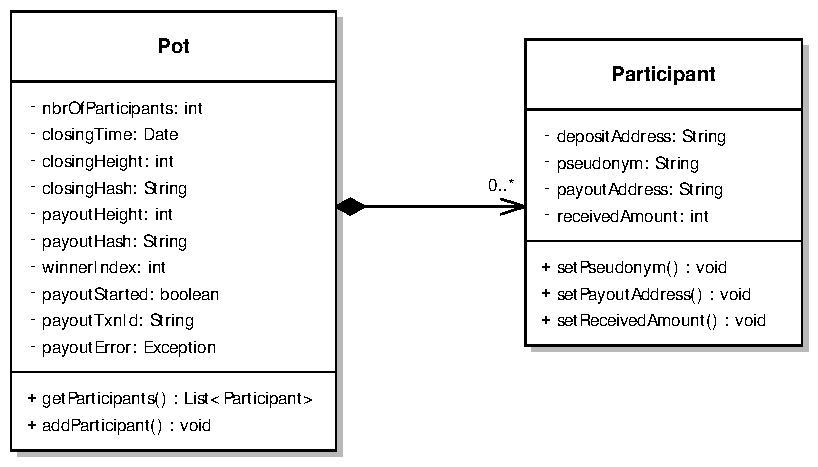
\includegraphics[width=1\linewidth]{Figures/umsetzung_btc/btc_datamodel}
\decoRule
\caption{Java Datenmodel Klassendiagramm}
\label{fig:btc_datenmodell}
\end{figure}

\subsection{Geschäftslogik}

Die Java Klassen der Glücksspielanwendung können, wie in Abbildung \ref{fig:btc_businesslogic} gezeigt, in 3 verschiedene Gruppen unterteilt werden. Das \textbf{Core Module} enthält die Klassen des Datenmodells und ein Interface mit dem die GUI Anwendung interagiert. Das Interface entkoppelt die Anzeigelogik der GUI von der Geschäftslogik der Kryptowährung. Die GUI Komponente bekommt von der Schnittstelle allgemeine Daten und kümmert sich nur um deren Anzeige.
Das \textbf{Bitcoin Service Module} enthält die gesamte kryptowährungsspezifische Geschäftslogik. \textbf{BitcoinJ} enthält alle Klassen und Interfaces die benötigt werden um mit dem Bitcoin Netzwerk zu interagieren und Daten aus der Blockchain auszulesen.

\begin{figure}[H]
\centering
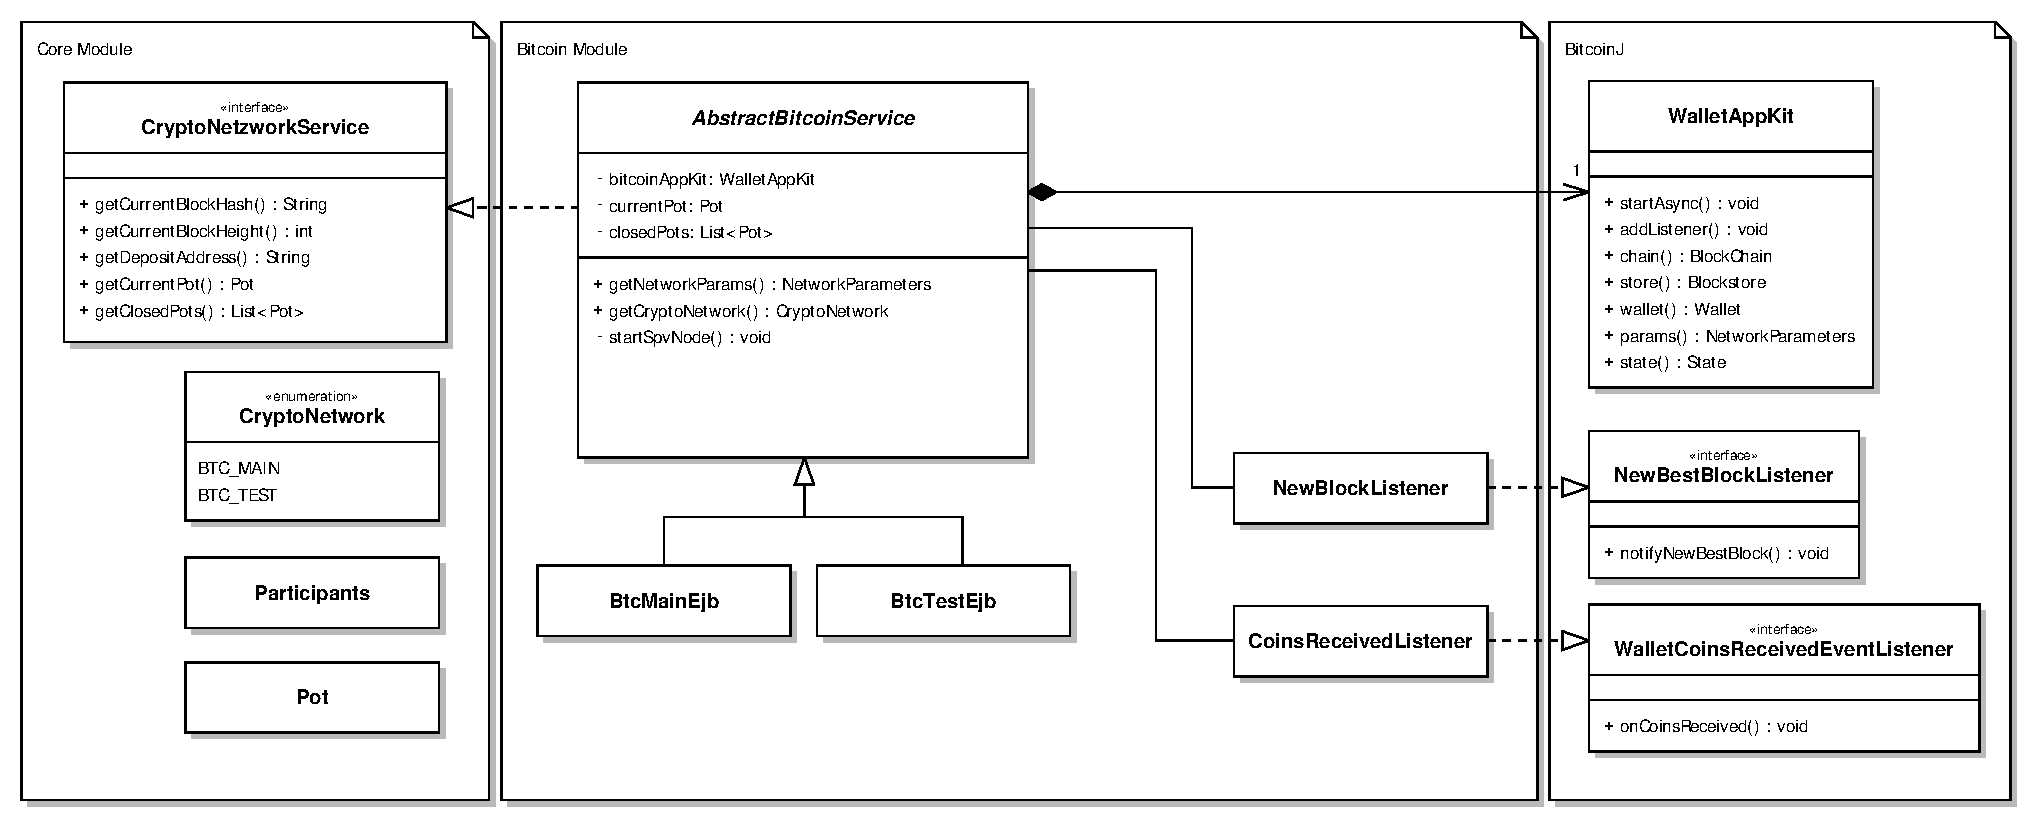
\includegraphics[width=1\linewidth]{Figures/umsetzung_btc/btc_businesslogic_pdf}
\decoRule
\caption{Java Geschäftslogik Klassendiagramm}
\label{fig:btc_businesslogic}
\end{figure}

\subsubsection{Start der Anwendung}
Beim Kompilieren der Anwendung wird über einen Konfigurationseintrag festgelegt, ob die Anwendung mit dem Bitcoin Haupt- oder Testnetzwerk interagieren soll.
Für das Hauptnetzwerk wird die Java Klasse \code{BtcMainEjb} verwendet. Für das Testnetwerk wird die Klasse \code{BtcTestEjb} verwendet. Beide Klassen verwenden die gleiche Implementierung der abstrakten Oberklasse \code{AbstractBitcoinService}. Diese wiederum implementiert das von der GUI Komponente verwendete Interface \code{CryptoNetworkservice}.

\begin{lstlisting}
import javax.ejb.Singleton;
import javax.ejb.Startup;
import org.bitcoinj.params.AbstractBitcoinNetParams;
import org.bitcoinj.params.MainNetParams;
import com.ossel.gamble.bitcoin.services.AbstractBitcoinService;
import com.ossel.gamble.core.data.enums.CryptoNetwork;
/**
 * Class will be excluded for the testnet jar via the maven jar plugin.
 */
@Startup
@Singleton
public class BtcMainEjb extends AbstractBitcoinService {
    @Override
    public CryptoNetwork getCryptoNetwork() {
        return CryptoNetwork.BTC_MAIN;
    }
    @Override
    public AbstractBitcoinNetParams getNetworkParams() {
        return MainNetParams.get();
    }
}
\end{lstlisting}


Die beiden Klassen \code{BtcMainEjb} und \code{BtcTestEjb} sind mit den Annotationen\code{@Startup} und \code{@Singleton} annotiert. Es handelt sich um sogenannte \textbf{E}nterprise \textbf{J}ava \textbf{B}eans. Dies bedeutet, dass der Applikationsserver diese eigenständig verwaltet und genau eine Instanz der Klasse beim Start der Applikation erzeugt. Beim Start wird dann die mit \code{@PostConstruct} annotierte \code{startSpvNode} Methode aufgerufen und abgearbeitet. Diese konfiguriert und startet das \code{WalletAppKit}, welches die zentrale Klasse zur Interaktion mit der BitcoinJ Bibliothek darstellt.

\begin{lstlisting}[basicstyle=\small] %or \tiny or \small or \footnotesize etc.
@PostConstruct
private void startSvpNode() {
    log.info("#### Start Bitcoin SPV Node  ####");
    currentPot = new Pot(2, 100000L);
    File walletDir = CoreUtil.getWalletDirectory();
    NetworkParameters params = getNetworkParams();
    String fileName = "bitcoin-" + params.getPaymentProtocolId();
    bitcoinAppKit = new WalletAppKit(params, walletDir, fileName) {
        @Override
        protected void onSetupCompleted() {
            log.info("#### Bitcoin SPV Node started ####");
        }
    };
    bitcoinAppKit.startAsync();
    waitUntilStarted(bitcoinAppKit);
    newBlockListener = new NewBlockListener(this);
    bitcoinAppKit.chain().addNewBestBlockListener(newBlockListener);
    coinReceivedListener = new CoinsReceivedListener(this);
    bitcoinAppKit.wallet().addCoinsReceivedEventListener(coinReceivedListener);
}
\end{lstlisting}

 In Zeile 4 wird zunächst ein neuer leerer Topf mit 2 Teilnehmern erzeugt. Anschließend wird das \code{WalletAppKit} erzeugt. Dazu bekommt dieses die gewünschten Netzwerkparameter und den Pfad zum Dateisystem in dem \code{BitcoinJ} die Blockchain- und Wallet-Daten speichern soll. Zeile 14 startet den durch das \code{WalletAppKit} repräsentierten SPV-Node. Anschließend wird dem \code{WalletAppKit} noch ein \code{NewBlockListener} und ein \code{CoinsReceivedListener} hinzugefügt, um auf neue Blöcke und eingehende Zahlungen zu reagieren.

\subsubsection{GUI Events}

Der folgende Code zeigt die Implementierung der Methoden die von der GUI Komponente aufgerufen werden.
\begin{lstlisting}
public Pot getCurrentPot() {
    return currentPot.clone();
}
public String getDepositAddress() {
    return bitcoinAppKit.wallet().freshAddress(KeyPurpose.RECEIVE_FUNDS).toString();
}
public String getCurrentBlockHash() {
    return bitcoinAppKit.chain().getChainHead().getHeader().getHash().toString();
}
public int getCurrentBlockHeight() {
    return bitcoinAppKit.chain().getChainHead().getHeight();
}
\end{lstlisting}


Die Methode \code{getCurrentPot} reicht in Zeile 2 die Daten des Topfs an die GUI Komponente weiter. Zeile 6 erzeugt eine neue Empfangsadresse und fügt einen weiteren möglichen Teilnehmer mit dieser Adresse der \code{possibleParticipants} Liste hinzu. Erst wenn eine Zahlung auf diese Adresse eingeht wird der Teilnehmer dem Topf hinzugefügt. Zeile 13 gibt den Blockhash des neusten Blocks der SPV Blockheader Kette zurück. Zeile 17 gibt die Blocknummer des neusten Blocks der SPV Blockheader Kette zurück.

\subsubsection{Bitcoin Netzwerk Events}

Immer wenn der SVP Node eine Transaktion auf eine vorher mittels der\\ \code{bitcoinAppKit.wallet().freshAddress()} erzeugten Adresse empfängt, wird die \code{onCoinsReceived} Methode der Klasse \code{CoinsReceivedListener} aufgerufen.

\begin{lstlisting}[basicstyle=\small]
@Override
public void onCoinsReceived(Wallet wallet, Transaction txn, Coin prevBalance, Coin newBalance) {
  log.debug("Transaction details: " + txn.toString());
  Coin value = txn.getValueSentToMe(wallet);
  Pot currentPot = service.getCurrentPot();
  if (currentPot.getExpectedBettingAmount() > value.getValue()) {
    log.warn("Player did not pay enough.");
    return;
  }
  List<Participant> participants = service.getPossibleParticipants();
  NetworkParameters params = service.getAppKit().params();
  for (TransactionOutput txnOutput : txn.getOutputs()) {
    Address a = txnOutput.getAddressFromP2PKHScript(params);
    String address = a.toString();
    for (Participant participant : participants) {
      String depositAddress = participant.getDepositAddress();
      if (depositAddress.equals(address)) {
        log.info("Received " + value.toFriendlyString() + " coins from " + participant.toString());
        participant.setReceivedAmount(value.getValue());
        String fromAddress = txn.getInput(0).getFromAddress().toString();
        participant.setPayoutAddress(fromAddress);
        wallet.addTransactionConfidenceEventListener(new TxnConfidenceListener(service, txn, participant));
      }
    }
  }
}
\end{lstlisting}


Zunächst wird in Zeile 6 geprüft, ob der eingegangene Zahlungsbetrag mindestens so hoch ist, wie von aktuellen Topf gefordert. Ist dies der Fall, iteriert die Methode über die Output Adressen\footnote{Eine detaillierte Beschreibung wie Bitcoin Transaktionen aufgebaut sind, liefert \cite{understanding_btc_txn}.} der Transaktion (Zeile 12) und prüft mit welcher Einzahlungsadresse der Teilnehmer (Teile 17) diese übereinstimmt. Handelt es sich bei der Output Adresse um keine Einzahlungsadresse eines Teilnehmers, wird diese ignoriert, da es sich um die Wechselgeldadresse eines Teilnehmers handeln muss\footnote{Bei Bitcoin können die einer Adresse zugewiesenen Währungseinheiten entweder ganz oder gar nicht ausgegeben werden. Daher ist es üblich eine vom Wallet kontrollierte Wechselgeldadresse in jeder Transaktion anzugeben.}. Hat man den Teilnehmer identifiziert, wird aus der Transaktion die Auszahlungsadresse berechnet und dem Teilnehmer der empfangene Geldbetrag gutgeschrieben (Zeile 19-21). Da es sich um eine gültige jedoch noch unbestätigte Transaktion handelt, wird der Teilnehmer erst nachdem die Transaktion in einen gültigen Block aufgenommen wurde zum Topf hinzugefügt. Zeile 22 erzeugt einen \code{TxnConfidenceListener} der diese Aufgabe übernimmt.

\begin{lstlisting}[basicstyle=\small]
@Override
public void onTransactionConfidenceChanged(Wallet wallet, Transaction txn) {
  if (txn.equals(targetTxn)) {
    log.debug("onTransactionConfidenceChanged Tx: " + txn.getHash());
    switch (txn.getConfidence().getConfidenceType()) {
      case PENDING:
        // unconfirmed but should be included shortly
        break;
      case BUILDING:
        // transaction is included in the best chain
        Pot currentPot = service.getCurrentPot();
        participant.setPotIndex(currentPot.getNbrOfParticipants());
        currentPot.addParticipant(participant);
        if (currentPot.isFull()) {
          service.closeCurrentPot(new Date());
        }
        wallet.removeTransactionConfidenceEventListener(this);
        break;
      case IN_CONFLICT:
        log.warn("possible double spend of txn " + txn.getHashAsString());
        break;
      case DEAD:
        log.warn("txn " + txn.getHashAsString()+ " won't confirm unless there is another re-org");
        wallet.removeTransactionConfidenceEventListener(this);
        break;
    }
  }
}
\end{lstlisting}


Die \code{onTransactionConfidenceChanged} Methode wird jedes mal aufgerufen wenn dem SPV-Client neue Daten zur Transaktion vorliegen. BitcoinJ unterscheidet zwischen vier verschiedenen \code{ConfidenceTypes}:
\begin{itemize}
\item PENDING: Bedeutet, dass die Transaktion noch unbestätigt ist und der SPV-Client darauf wartet, dass er einen Block erhält in dem die Transaktion enthalten ist.
\item BUILDING: Bedeutet, dass die Transaktion bereits in die Blockchain aufgenommen wurde. Durch den Aufruf von\\ \code{transaction.getConfidence().getAppearedAtChainHeight()} kann man abfragen, wie tief die Transaktion bereits in der Blockchain steckt. Diese Methode gibt zurück, wie viele Blöcke bereits auf den Block, der die Transaktion enthält, aufbauen. Die Glücksspielanwendung betrachtet eine Transaktion ab dem Zeitpunkt als final, ab dem sie in einen gültigen Block aufgenommen wurde.\footnote{Vor der Auszahlung des Gewinns kann die Anwendung erneut nachprüfen, ob es eine Restrukturierung der Blockchain durch einen Blockchainfork gab. Dadurch stellt sie sicher, dass alle Transaktionen Teil der längsten Blockkette geworden sind.} Geschieht dies, wird der Teilnehmer der Transaktion in den Topf hinzugefügt. \todo{Methode in COde einbauen unter BUILDING und dort über konfigurationswert festlegbar machen ab wann man die TXN akzeptiert.}
\item IN CONFLICT: In diesem Fall hat der SPV-Client zwei Transaktionen erhalten, die versuchen den gleichen Transaction-Output auszugeben. Man spricht von einem sogenannten ''double spend'' Angriff. 
\item DEAD: Transaktionen die diesen Status erhalten, können nicht mehr bestätigt werden, außer es kommt zu einer Blockchain Restrukturierung.\todo{Kann dieser Status wirklich vorkommen?}
\end{itemize}

Immer wenn der SVP Node einen neuen besten Block empfängt, den er vorne an die Blockheader Kette anhängen kann, wird die \code{notifyNewBestBlock} Methode aufgerufen.
\begin{lstlisting}[basicstyle=\small]
@Override
public void notifyNewBestBlock(StoredBlock block) throws VerificationException {
    log.info("New Block height = " + block.getHeight() + " hash = "
            + block.getHeader().getHash().toString());
    List<Pot> unfinishedPots = getUnfinishedPots(service.getClosedPots());
    for (Pot pot : unfinishedPots) {
        long potId = pot.getCreateTime().getTime();
        int payoutBlockHeight = pot.getPayoutBlockHeight();
        if (payoutBlockHeight > block.getHeight()) {
            log.info("Pot[" + potId + "] can not be handled yet.");
        } else if (payoutBlockHeight == block.getHeight()) {
            log.info("Pot[" + potId + "] select temorary Winner.");
            Block tmpPayoutBlock = new ExtendedBlock(block.getHeader().getHash().toString());
            pot.setPayoutBlock(tmpPayoutBlock);
            selectWinner(pot, tmpPayoutBlock);
        } else {
            log.info("Pot[" + potId + "] select final winner.");
            try {
               StoredBlock correctBlock = getPastBlock(payoutBlockHeight, block);
               String payoutBlockHash = correctBlock.getHeader().getHash().toString();
               Block finalPayoutBlock = new ExtendedBlock(payoutBlockHash);
               pot.setPayoutBlock(finalPayoutBlock);
               Participant winner = selectWinner(pot, finalPayoutBlock);
               log.info(winner.getDepositAddress() + " wins pot[" + potId + "].");
               startPayoutThread(pot);
            } catch (BlockStoreException e) {
               log.info("Couldn't select final winner of Pot[" + potId + "]:" + e.getMessage(), e);
            }
        }
    }
}
\end{lstlisting}



Diese Methode iteriert über alle bereits geschlossenen Töpfe, für die noch keine Auszahlung stattgefunden hat und unterscheidet dabei 3 Fälle:
\begin{enumerate}
\item Die Blocknummer des neusten Blocks ist kleiner als die Blocknummer, die den Topf entscheidet. In diesem Fall passiert nichts.
\item Der neue Block entscheidet den Topf, da die Blocknummer des Blocks gleich der \code{PayoutHeigth} des Topfs ist. Der Gewinner des Topfs wird selektiert, es findet allerdings keine Auszahlung statt. Die finale Auszahlung findet aus Sicherheitsgründen erst im nächsten Fall statt.
\item In diesem Fall gibt es mindestens einen Block, der auf dem Payout-Block des Topfs aufbaut. Ab diesem Zeitpunkt betrachtet die Anwendung den Gewinner als final.\footnote{An dieser Stelle kann man natürlich auch aus Sicherheitsgründen noch mehrere Blöcke abwarten, bevor die Anwendung eine Auszahlung startet. Ab einer Tiefe von 6 Blöcken gelten Bitcoin Zahlungen als irreversibel. Bei sehr hohen Zahlungen ist es empfehlenswert so lange abzuwarten.} Daher wird der Gewinner des Topfs überschrieben und die Auszahlung in einem neuen \code{Thread} gestartet.
\end{enumerate}

Die Klasse \code{ExtendedBlock} teilt den Blockhash zur Anzeige in der GUI in die Werte \code{perfix}, \code{lastDigit} und \code{suffix}. Die Variable \code{lastDigit} speichert die letzte numerische Stelle des Blockhashs und wird zur Gewinnerauswahl verwendet.

\begin{lstlisting}[basicstyle=\small]
public class ExtendedBlock extends Block {

    private String prefix;
    private String suffix;

    public ExtendedBlock(String blockHash) {
        super(blockHash, -1);
        int position = blockHash.length() - 1;
        while (position > 0) {
            char c = blockHash.charAt(position);
            int value = (int) c;
            if (value >= 48 && value <= 57) {// numeric
                this.lastDigit = Integer.parseInt(String.valueOf(c));
                break;
            }
            position--;
        }
        this.prefix = blockHash.substring(0, position);
        this.suffix = blockHash.substring(position + 1, blockHash.length());
    }
}
\end{lstlisting}







\subsubsection{Auszahlungen}
Auszahlung werden in einem eigenen Thread abgehandelt. Die Klasse \code{PayoutThread} ruft dazu die \code{payout} Methode auf.
\begin{lstlisting}
private void payout(Pot pot) throws InsufficientMoneyException, InterruptedException, ExecutionException {
    if (pot.isPayoutStarted()) {
        log.error("Payout already started: " + pot.getPayoutTxnId() + " - "
                + pot.getPayoutError());
    } else {
        pot.setPayoutStarted(true);
        Address winnerAddress = new Address(bitcoinService.getNetworkParams(),
                pot.getWinner().getPayoutAddress());
        Coin potValue = Coin.SATOSHI
                .multiply(pot.getParticipants().size() * pot.getExpectedBettingamount());
        Wallet.SendResult result = bitcoinService.getAppKit().wallet()
                .sendCoins(bitcoinService.getAppKit().peerGroup(), winnerAddress, potValue);
        String txnId = result.tx.getHash().toString();
        pot.setPayoutTxnId(txnId);
        log.info("Payout TXN ID = " + txnId);
        Transaction transaction = result.broadcastComplete.get();
        log(transaction);
    }
}
\end{lstlisting}


Die Methode prüft zunächst, dass die Auszahlung noch nicht gestartet wurde. Ist dies der Fall, wird der auszuzahlende Betrag berechnet und an die Adresse des Gewinners überwiesen. Anschließen wird die ID der Auszahlungstransaktion in den Topf geschrieben. Während der Auszahlung können von BitcoinJ 3 verschiedene Fehler auftreten:
\begin{enumerate}
\item InsufficientMoneyException: Falls die von der Wallet verwalteten Adressen nicht genug Bitcoin für die Auszahlung besitzen.
\item InterruptedException: Falls der Java Thread unterbrochen wird.
\item ExecutionException: Falls es zu einem unerwarteten Fehler bei der Ausführung kommt.
\end{enumerate}
Sollte es bei der Auszahlung ein Problem geben, wird die Exception gefangen und im \code{Pot} Objekt unter \code{payoutError} abgespeichert.

\subsection{Grafische Benutzeroberfläche}\label{ssec:btc_gui}

Die graphische Oberfläche der Anwendung ist mit dem Tapestry Framework von Apache realisiert. Da die GUI Komponente nur die Daten visualisiert, wird an dieser Stelle auf eine genauere Betrachtung verzichtet und lediglich die Benutzeroberfläche gezeigt.


\begin{figure}[H]
\centering
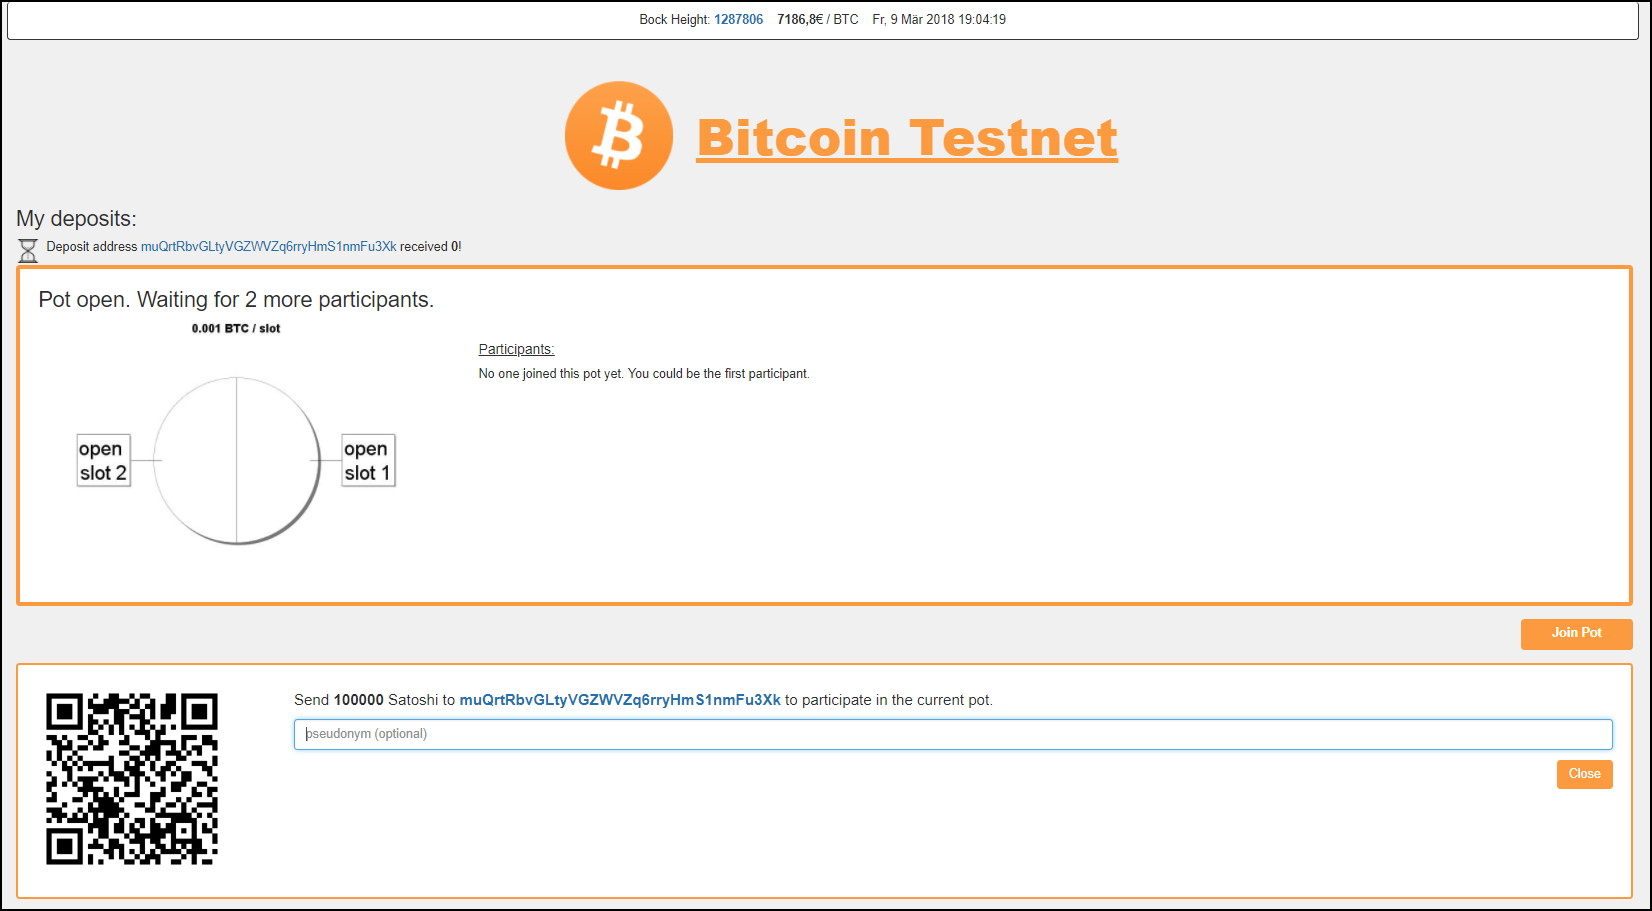
\includegraphics[width=1\linewidth]{Figures/btc_gui/pot_open_empty}
\decoRule
\caption{Leerer Topf}
\label{fig:pot_open_empty}
\end{figure}
Abbildung \ref{fig:pot_open_empty} zeigt einen Topf mit 2 freien Plätzen. Um dem Spiel beizutreten, muss der Spieler den Betrag von 0,001 Bitcoin an die angezeigte Adresse senden. Der angezeigte QR-Code erleichtert dem Spieler die Übertragung dieser Daten in das Überweisungsformular seines Smartphone Wallets. Das \textbf{B}itcoin \textbf{I}mprovement \textbf{P}roposal Nummer 21 \cite{bip21} legt fest, in welchem Format diese Daten kodiert werden müssen, damit beliebige Bitcoin Clients diese auslesen und interpretieren können. 
Folgende Daten sind in dem QR Code enthalten:\\ ''bitcoin:muQrtRbvGLtyVGZWVZq6rryHmS1nmFu3Xk?amount=0.001''

\vspace{1cm}
\begin{minipage}{0.48\textwidth}
\begin{figure}[H]
\centering
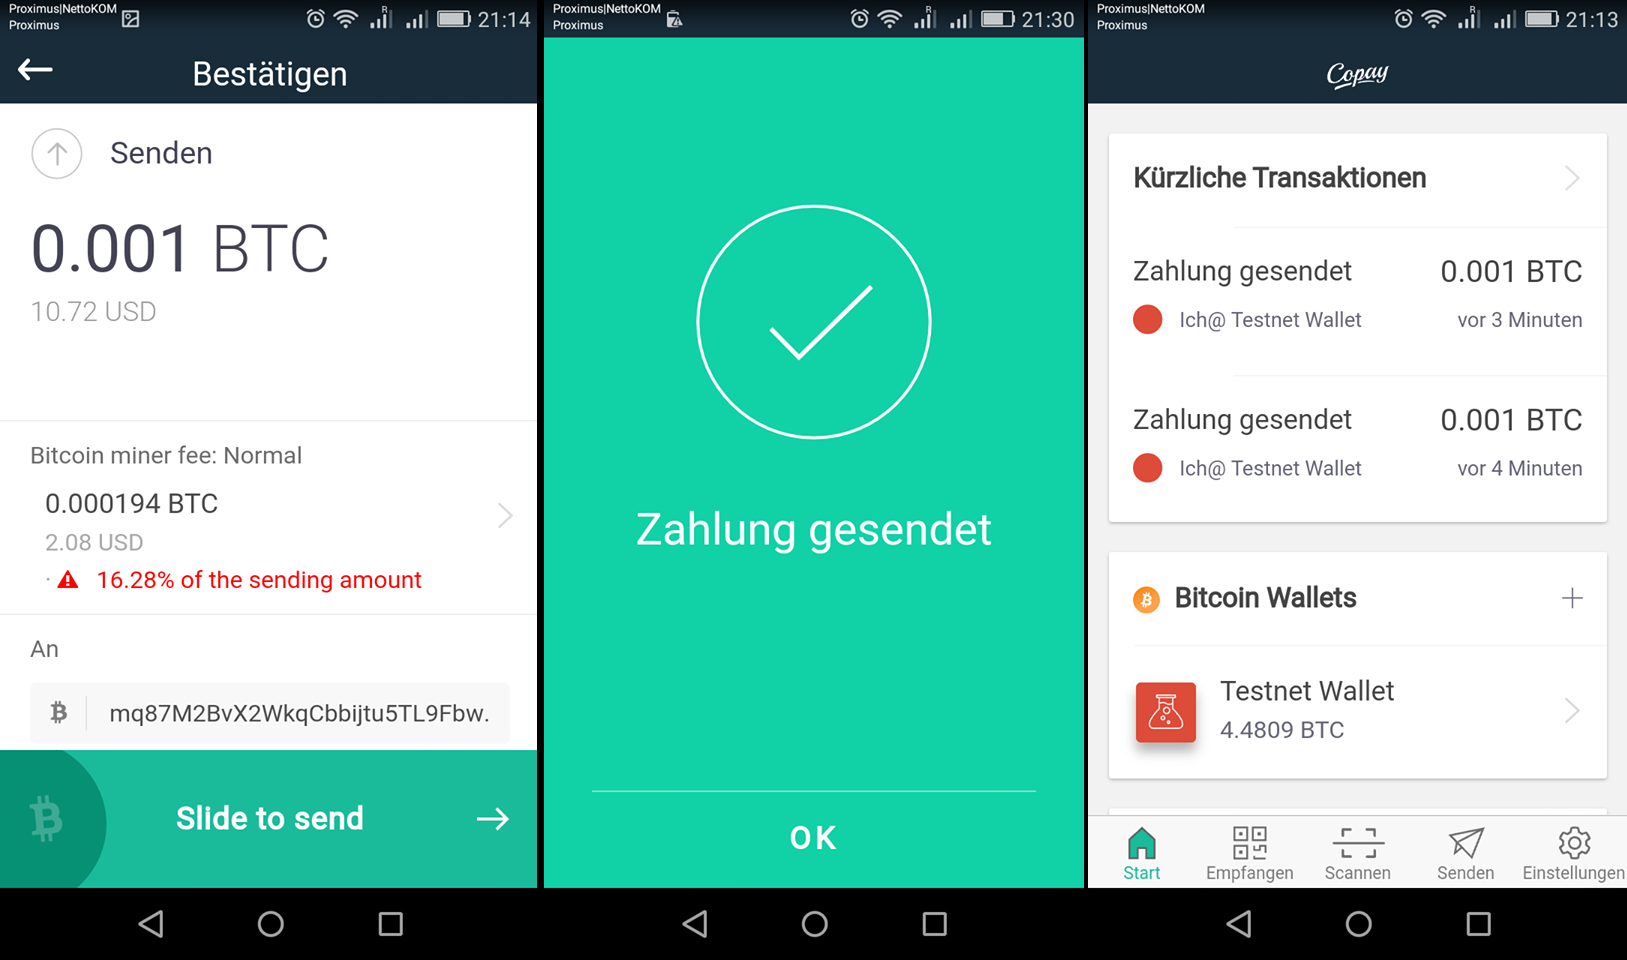
\includegraphics[width=1\linewidth]{Figures/btc_gui/handy_send}
\decoRule
\caption{Smartphone Überweisungsformular}
\label{fig:handy_send}
\end{figure}
\end{minipage}
\begin{minipage}{0.48\textwidth}
\begin{figure}[H]
\centering
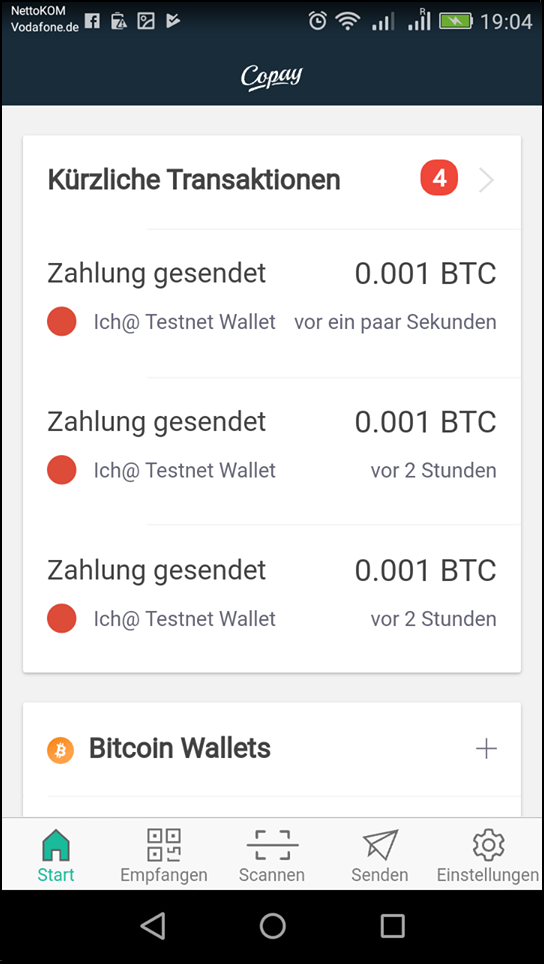
\includegraphics[width=1\linewidth]{Figures/btc_gui/handy_confirm}
\decoRule
\caption{Zahlungsbestätigung}
\label{fig:handy_confirm}
\end{figure}
\end{minipage}

Abbildungen \ref{fig:handy_send} und \ref{fig:handy_confirm} zeigen das Bitcoin CoPay Wallet\footnote{\url{https://copay.io/}}. Dieses erlautb, neben Zahlungen im Bitcoin Hauptnetzwerk, auch Zahlungen an das Bitcoin Testnetz zu senden. Nachdem der Benutzer den QR-Code der Glücksspielanwendung mit seinem Smartphone abgescannt hat, erscheint sowohl der Betrag als auch die Empfangsadresse vorausgefüllt im Überweisungsformular. Die Wallet berechnet automatisch eine passende Transaktionsgebühr. Der Spieler überprüft lediglich die Adresse und den Betrag und  autorisiert anschließend die Zahlung.

\begin{figure}[H]
\centering
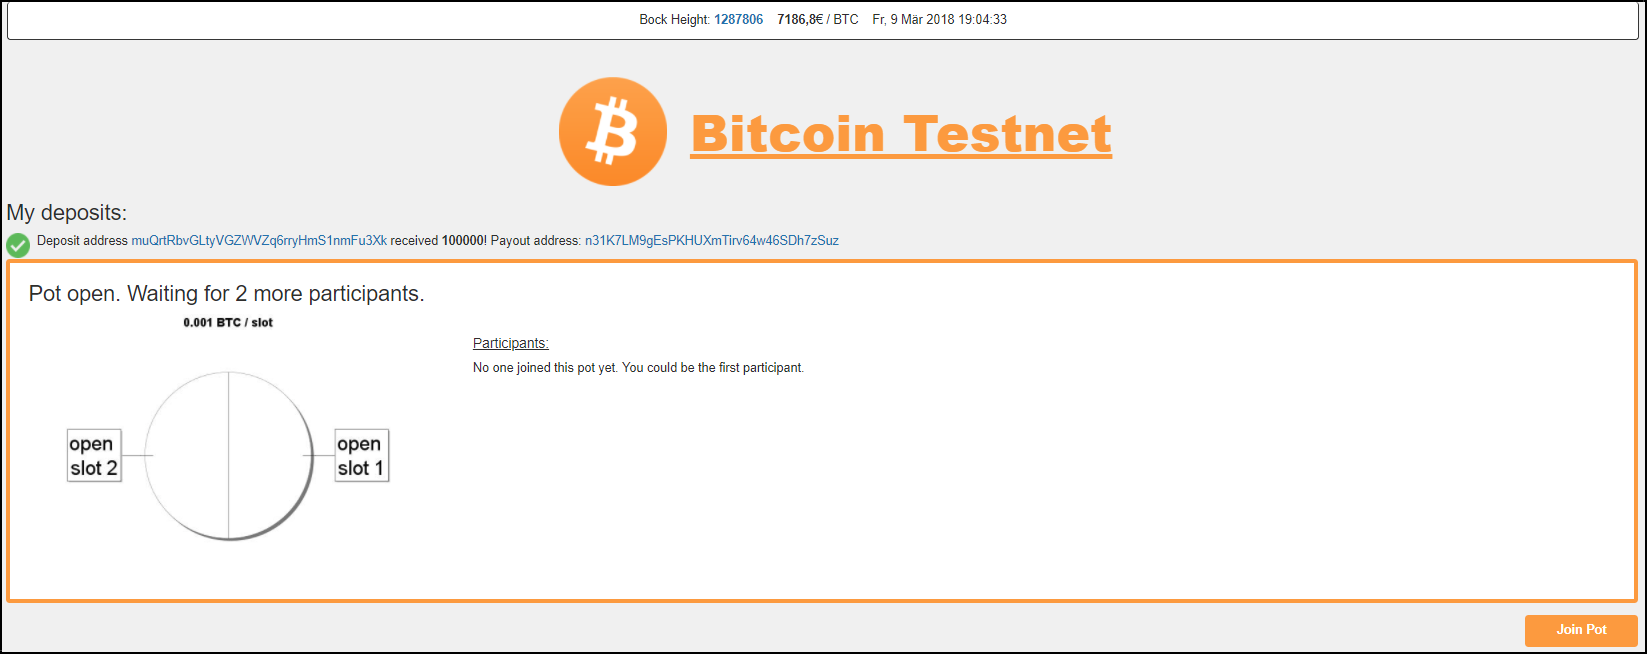
\includegraphics[width=1\linewidth]{Figures/btc_gui/pot_open_payment_received}
\decoRule
\caption{Transaktion empfangen}
\label{fig:pot_open_payment_received}
\end{figure}

Sobald die Anwendung die Transaktion empfängt, zeigt sie dies durch einen grünen Haken an. Dies ist in Abbildungen \ref{fig:pot_open_payment_received} zu sehen. Zu diesem Zeitpunkt handelt es sich um eine unbestätigte Transaktion, die noch in keinen Bock der Blockchain aufgenommen wurde.

\begin{figure}[H]
\centering
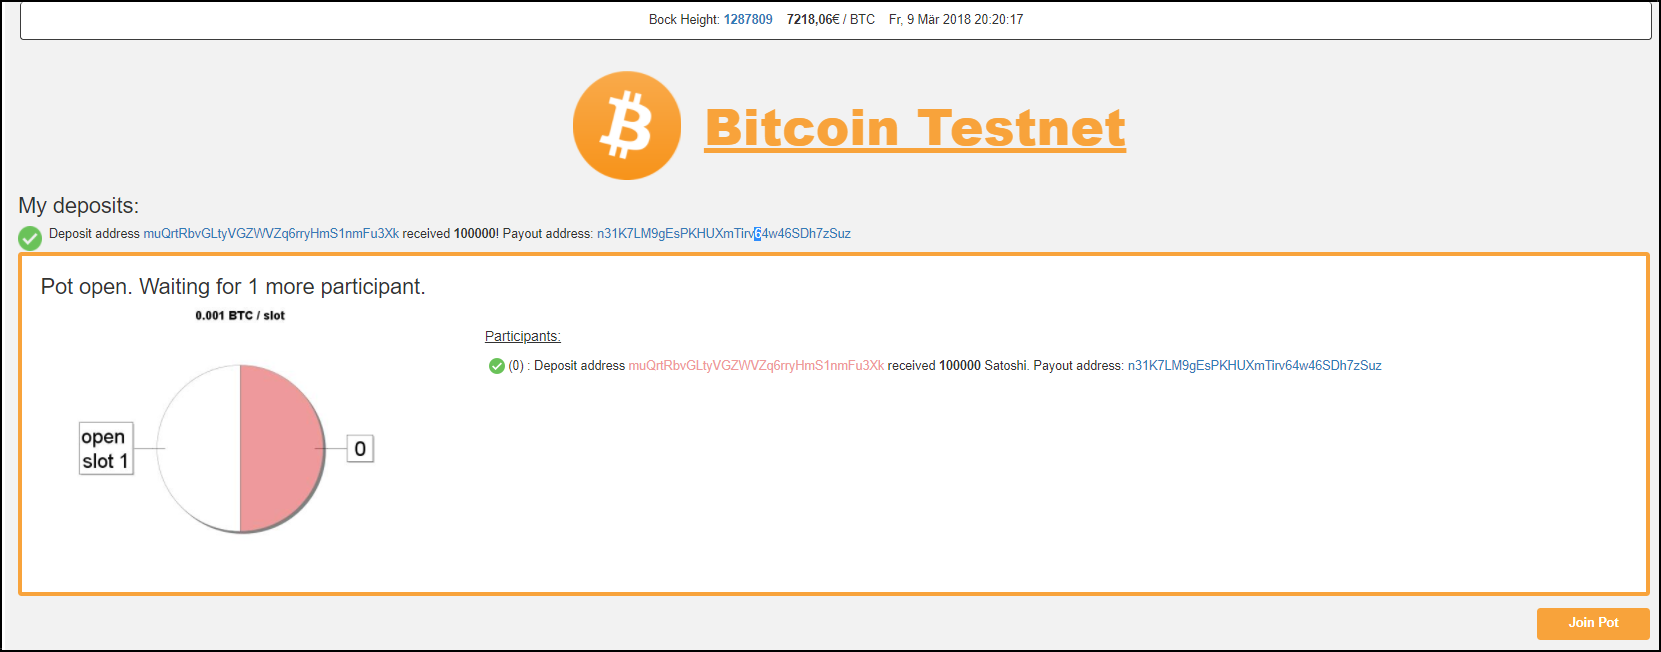
\includegraphics[width=1\linewidth]{Figures/btc_gui/pot_open_p1_confirmed}
\decoRule
\caption{Spieler zu Topf hinzugefügt.}
\label{fig:pot_open_p1_confirmed}
\end{figure}
Sobald die Anwendung einen neuen Block empfängt, der die Transaktion enthält, gilt die Transaktion als bestätigt und der Spieler wird zum Topf hinzugefügt. Nun gibt es nur noch einen offenen Platz im Topf.

\begin{figure}[H]
\centering
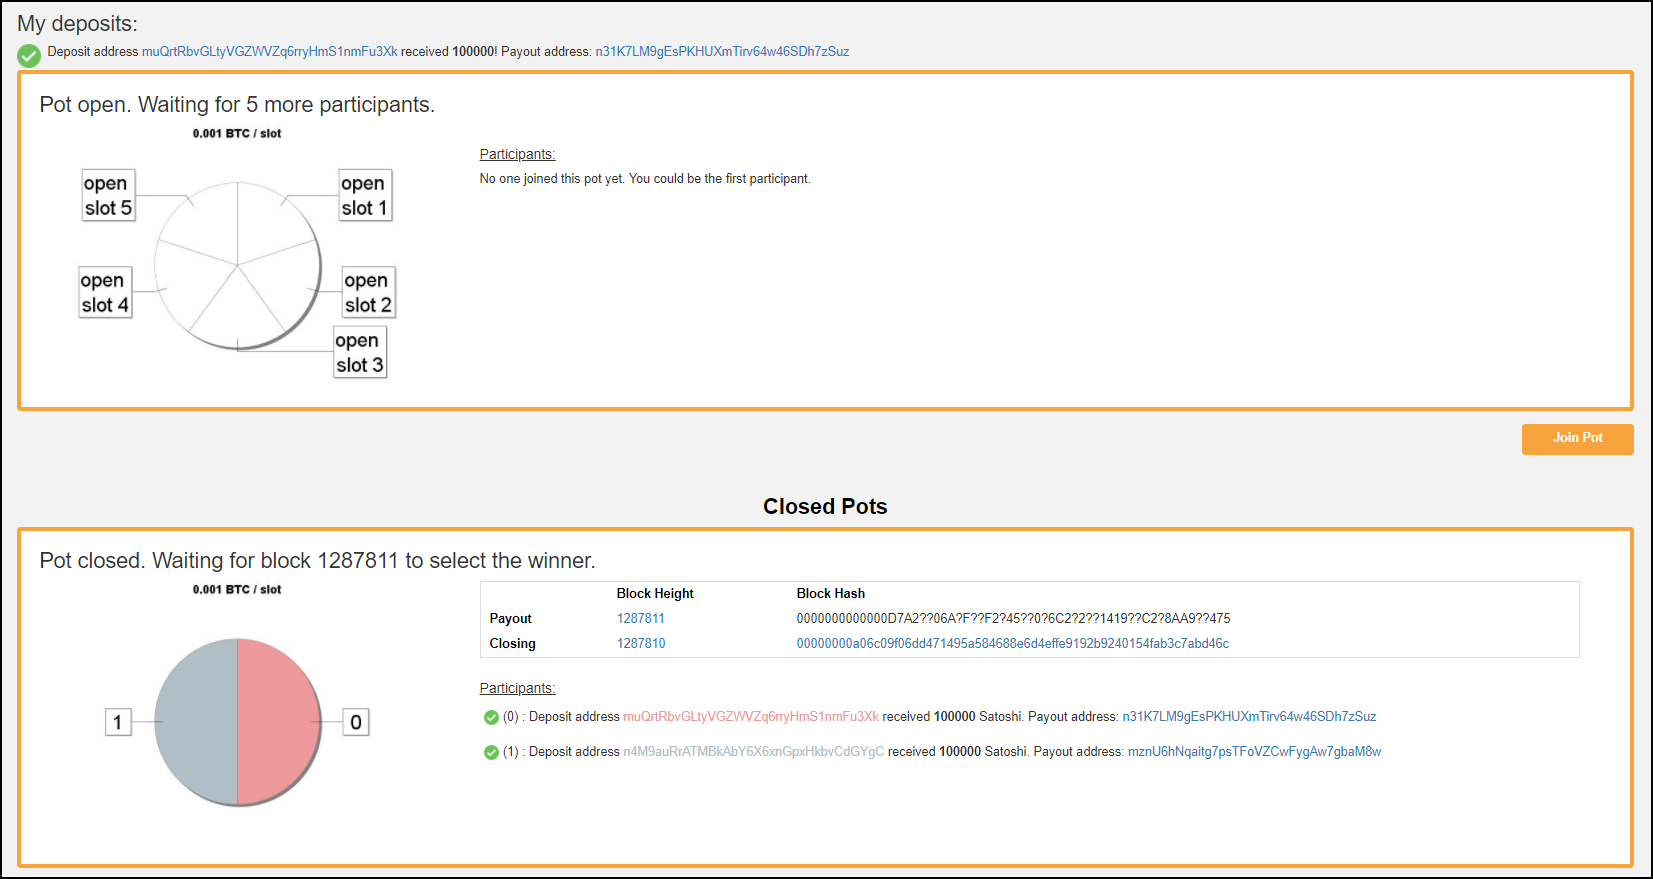
\includegraphics[width=1\linewidth]{Figures/btc_gui/pot_closed}
\decoRule
\caption{Topf geschlossen}
\label{fig:pot_closed}
\end{figure}

Nachdem ein weiterer Spieler in den Topf eingezahlt hat, ist der Topf voll. Die Anwendung schließt den aktuellen Topf und öffnet einen neuen Topf. Die Anwendung erstellt zufällig entweder einen Topf mit 2, 5 oder 10 freien Plätzen. In einer real eingesetzten Glücksspielanwendung würden alle Spielvarianten parallel angeboten. Der in Abbildung \ref{fig:pot_closed} gezeigte neue Topf hat fünf freie Plätze. Die Anwendung wartet nun auf den \code{Payout}-Block, um den Gewinner des geschlossenen Topfs festzulegen. Da der Blockhash noch nicht feststeht, zeigt die Anwendung die Animation eines sich sehr schnell wechselnden Blockhashs an, der mehrere Fragezeichen enthält.

\begin{figure}[H]
\centering
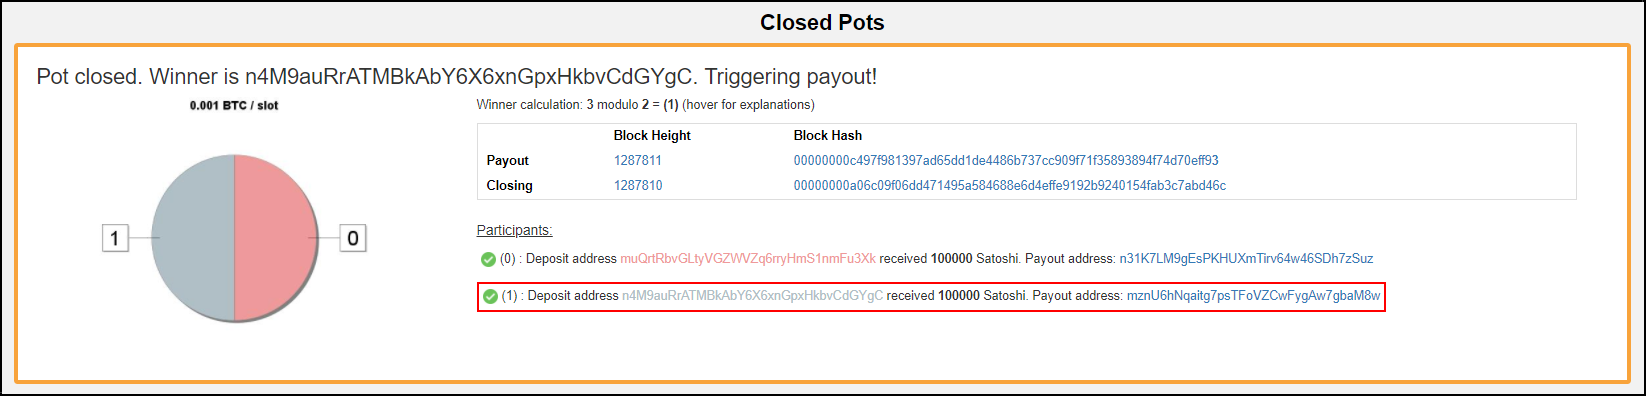
\includegraphics[width=1\linewidth]{Figures/btc_gui/pot_closed_triggering_payout}
\decoRule
\caption{Gewinner ermittelt}
\label{fig:pot_closed_triggering_payout}
\end{figure}
Sobald der entscheidende Block empfangen wird, wird der voraussichtliche Gewinner des Topfs durch ein rotes Rechteck markiert. Außerdem zeigt die Anwendung durch welche Berechnung der Gewinner festgelegt wurde. Nun wartet die Anwendung bis ein weiterer Block gefunden wird, bevor sie die Auszahlung an den Gewinner startet. 

\begin{figure}[H]
\centering
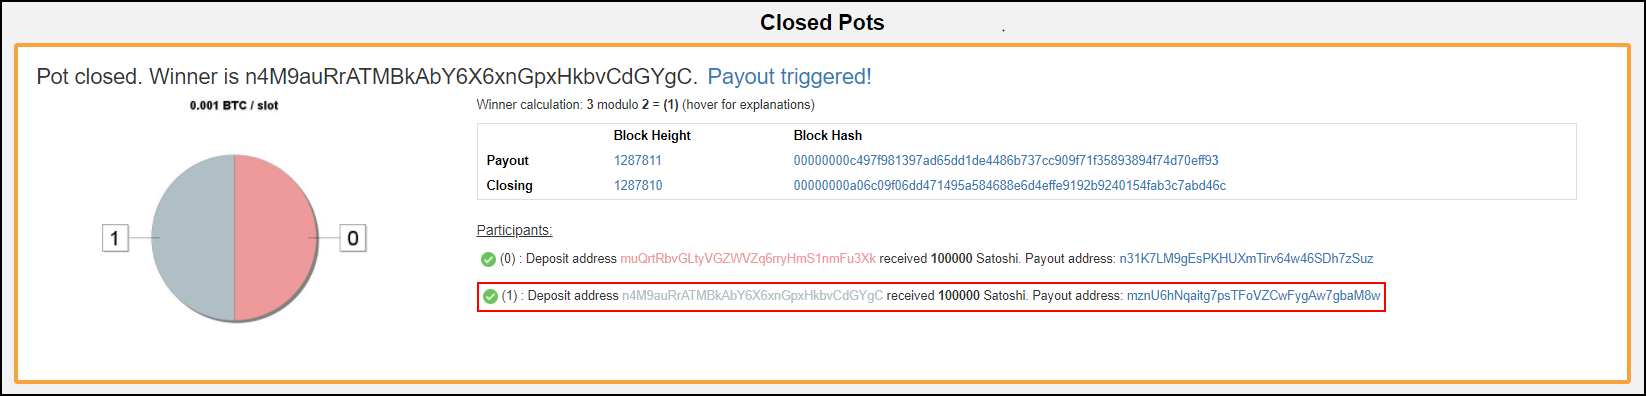
\includegraphics[width=1\linewidth]{Figures/btc_gui/pot_closed_payout_finished}
\decoRule
\caption{Auszahlung beendet}
\label{fig:pot_closed_payout_finished}
\end{figure}

Klickt der Benutzer auf den \emph{Payout triggered} Link aus Abbildung \ref{fig:pot_closed_payout_finished}, gelangt er zu einem Blockexplorer. Dieser zeigt ihm die Transaktionsdetails an. Eine genauere Betrachtung findet in Abschnitt \ref{sssec:Auszahlungstransaktion} statt. 
\section{Evaluation}
\subsection{Prüfung der Anforderungen}\label{btc_evaluation}%Anforderungserfüllung}

Dieser Abschnitt behandelt in wie weit das beschriebene Konzept die in \ref{anforderungen} aufgelisteten Anforderungen erfüllt. Die jeweilige Anforderung wird zunächst wiederholt und anschließend genauer untersucht.

\subsubsection{1) Transparente Einzahlungen}
\textit{Die Einzahlung jedes Endnutzers ist für jeden anderen Endnutzer nachprüfbar.}\\\\
Diese Anforderung ist erfüllt, da jede Transaktion in der lokalen Datenbank jedes Peet-to-Peer Netzwerkteilnehmers aufgezeichnet wird. 
Auf der Webseite \cite{blockchain_info} kann man die Bitcoin Blockchain mithilfe eines sogenannten Blockchain-Explorers durchsuchen. Mit diesem Werkzeug kann man die Blöcke und die darin enthaltenen Transaktionen untersuchen. Nutzt man den Explorer einer Drittpartei, muss man darauf vertrauen, dass dieser auch den ''wahren'' Status der Blockchain anzeigt. Um dieses Risiko zu vermeiden kann jeder Teilnehmer mithilfe eines eigenen Bitcoin Full Nodes am Netzwerk teilnehmen. Dieser speichert die gesamte Blockchain und prüft alle Transaktionen und Blöcke gegen die Konsensregeln.\\
Der Bitcoin Full Node stellt eine API bereit, über die man den aktuellen Status der Blockchain abfragen kann. Der Befehl \textit{getblockchaininfo} liefert den aktuellen Zustand der Blockchain zurück. Dieser beinhaltet die Blocknummer des neusten Blocks und dessen Blockhash. Der Befehl \textit{gettransaction} gefolgt von der Transaktions-ID liefert Details über diese Transaktion. Die Webseite \cite{btc_api} dokumentiert diese Schnittstelle detailliert. 

\subsubsection{2) Gewinnerauswahl durch Zufallsfaktor}
\textit{Die Auswahl des Gewinners ist von einem zufälligen Faktor abhängig, auf den weder die Anwendung noch die Endnutzer einen Einfluss haben.}\\\\
Diese Anforderung wird nur bedingt erfüllt, da ein Teilnehmer des Peer-to-Peer Netzwerks sowohl ein Spieler als auch ein Miner sein kann. Ist dies der Fall besteht die Möglichkeit, dass der Miner einen validen Blockhash verwirft, sobald er merkt, dass er durch diesen Blockhash nicht zum Gewinner des Geldtopfes wird. Verwirft der Teilnehmer einen Blockhash, riskiert er den dadurch ausgeschütteten Blockreward. Ein solcher Angriff ist für einen Miner nur rentabel, falls die Einnahmen des Glücksspiels hoch genug sind um den potentiellen Verlust des Blockrewards zu kompensieren. Die Rentabilität eines solchen Manipulationsversuchs hängt außerdem von der Hashrate des Miners ab, da diese bestimmt, mit welcher Wahrscheinlichkeit der Miner einen weiteren gültigen Block findet. Der Abschnitt \ref{btc_eval_miner} betrachtet dieses Szenario detailliert. %und kommt zu dem Schluss, dass Töpfe mit einem Einsatz von bis zu circa 60000 Euro als sicher anzusehen sind                                                                                                                                                                                                                                                                                                                                                                                                                                                                                                                                                                                                                                                                                                                                                         

\subsubsection{3) Nachprüfbarkeit des Zufallsfaktor}
\textit{Jeder Endnutzer kann die Echtheit des zufälligen Faktors eigenständig nachprüfen.}\\\\
Da das Verfahren der Gewinnerauswahl im Vorhinein festgelegt ist und die Reihenfolge der Einzahlungstransaktionen in der Blockchain festgeschrieben steht, kann jeder Teilnehmer die Berechnung des Gewinners eigenständig nachvollziehen. Der Blockhash, der die Grundlage für die Gewinnerauswahl liefert, kann durch die Verwendung eines Bockchain-Explorers oder eines Full Nodes nachgeprüft werden. 
\subsubsection{4) Transparente Auszahlungen}
\textit{Die Auszahlung an den Gewinner muss transparent und somit für jeden Endnutzer nachprüfbar sein.}\\\\
Genau wie die Einzahlungen ist auch die Auszahlung für jeden Spieler mithilfe eines Blockchain-Explorers oder eines Bitcoin Full Nodes möglich. Jeder Teilnehmer kann somit für alle bereits abgeschlossenen Spiele nachprüfen, ob die Anwendung sich korrekt verhalten und eine Auszahlung getätigt hat. 
\subsubsection{5) Fairheit des Spiels}
\textit{Jeder Endnutzer besitzt die gleiche Gewinnwahrscheinlichkeit und niemand wird benachteiligt}.\\\\
Die Zuordnung der Spieler auf die Gewinnzahlen ist durch die Reihenfolge der Transaktionen in der Blockchain festgeschrieben. Eine nachträgliche Veränderung dieser Reihenfolge ist weder durch die Nutzer, noch durch die Glücksspielanwendung möglich.\footnote{Eine Veränderung der Reihenfolge ist nur durch einen sogenannten Blockchain-Fork möglich. (siehe Abschnitt \ref{sssec:btc_fork})}

Damit keiner der Spieler einen Vorteil hat, muss jeder Topf-Platz die gleiche Gewinnwahrscheinlichkeit haben.
Dies ist gegeben, falls jeder Teilnehmer die gleiche Anzahl Gewinnzahlen zugeordnet bekommt und falls das Auftreten jeder Gewinnzahl die gleiche Wahrscheinlichkeit besitzt. Durch die Einschränkung der Topfgröße auf 2, 5 und 10 Teilnehmer bekommt jeder Spieler durch die Modulo-Funktion genau gleich viele Gewinnzahlen zugeordnet. Die Monte-Carlo-Simulation aus Abschnitt \ref{btc_distribution} legt nahe, dass die letzte Dezimalziffer der Werte der von Bitcoin verwendeten SHA-256 Hashfunktion gleichverteilt sind. Somit ist das Auftreten jeder Gewinnzahl gleich wahrscheinlich und die Anforderung erfüllt.

\subsection{Gewinnerauswahl}\label{btc_gewinnerauswahl}
Die Gewinnerauswahl kann entweder durch den gesamten Blockhash-Wert oder auf Basis der letzten Blockziffer vorgenommen werden.
Beide Methoden haben Vor- und Nachteile. Variante eins erlaubt beliebige Topfgrößen, ist dafür aber schwieriger für den Endnutzer zu verifizieren. Die Verifizierung erfordert eine Modulo-Rechnung mit einer sehr großen Zahl. Variante zwei ist dagegen leicht zu verifizieren, erlaubt allerdings nur die Topfgrößen zwei, fünf und zehn. Bei der Topfgröße von zwei sind beiden Spielern fünf Gewinnzahlen zugeordnet. Bei der Topfgröße von fünf besitzt jeder Teilnehmer genau 2 Gewinnzahlen. Bei einer Topfgröße von zehn wird jedem Teilnehmer genau eine Gewinnzahl zugeordnet. 
Nimmt man hingegen eine Topfgröße von 3,4,6,7,8 und 9 führt dies dazu das manche Teilnehmer eine signifikant höhere Gewinnchance haben.
Bei der Topfgröße von 3 sind die Gewinnzahlen durch die Modulo-Funktion folgendermaßen verteilt:
\begin{itemize}
\item Spieler 1 hat die Gewinnzahlen 0, 3, 6 und 9.
\item Spieler 2 hat die Gewinnzahlen 1, 4 und 7.
\item Spieler 3 hat die Gewinnzahlen 2, 5 und 8.
\end{itemize}
Somit hat Spieler 1 eine Gewinnwahrscheinlichkeit von $\frac{4}{10}$, Spieler 2 und 3 hingegen nur eine Gewinnwahrscheinlichkeit von $\frac{3}{10}$. Es kommt also vor, dass eine Teilmenge der Spieler genau eine Gewinnzahl mehr als der Rest der Teilnehmer hat.

Nimmt man den gesamten Blockhash zur Gewinnerauswahl ist die dadurch entstehende Ungerechtigkeit verschwindend gering und kann vernachlässigt werden. Dies ist der Fall, da die aus dem Blockhash resultierende Dezimalzahl in der Praxis sehr groß ist und jeder Spieler somit mehrere Millionen von Gewinnzahlen hat.

\subsection{Verteilung der Blockhash-Werte}\label{btc_distribution}
Der Blockhash eines Blocks wird durch die verwendete kryptographische Hashfunktion der Kryptowährung festgelegt. Die Verteilung der Werte wird somit von der verwendeten kryptographische Hashfunktion festgelegt.\\
Eine kryptografische Hashfunktion ist eine stark kollisionsresistente Einweg-Hashfunktion.\\
Eine Hashfunktion h heißt
\begin{itemize}
\item \textit{Einwegfunktion} genau dann, wenn es schwierig ist, zu gegebenem $_{Y0}$ ein $_{X0}$ zu finden mit $h(x_{0}) = y_{0}$.
\item \textit{schwach kollisionsresistent} genau dann, wenn es schwierig ist, zu einem gegebenen $x$ ein $x' \neq x$ zu finden mit $h(x) = h(x')$.
\item \emph{stark kollisionsresistent} genau dann, wenn es schwierig ist, $x$ und $x'$ zu finden
mit $x \neq x'$ und $h(x) = h(x')$.
\end{itemize}Die Eigenschaften der starken Kollisionsresistenz und der Einwegfunktion sagen nichts über die Verteilung der resultierenden Werte aus. Bei der Auswahl der Kryptowährung muss also gesondert auf die Verteilung der verwendete Hashfunktion geachtet werden. Sollte die verwendete kryptographische Hashfunktion keine Gleichverteilung liefern, kann der Blockhash dennoch den nötigen Zufall liefern indem dieser mit einer geeigneten Hashfunktion erneut gehasht wird.\\\\
Bitcoin verwendet die kryptographische Hashfunktion SHA256.
Die folgende Monte-Carlo-Simulation legt nahe, dass die Resultate der SHA256 gleichverteilt sind.
\begin{verbatim}
h=SHA256 n=1000000
for i 1 -> n
    hash = h(i);
    result[lastDigit(hash)]++
\end{verbatim}
\begin{minipage}{0.5\textwidth}
\begin{verbatim}
Ausgabe:
result[0] =  99765
result[1] = 100488
result[2] =  99913
result[3] = 100745
result[4] = 100272
result[5] =  99649
result[6] =  99430
result[7] =  99788
result[8] =  99666
result[9] = 100284
\end{verbatim}
\end{minipage}
\begin{minipage}{0.5\textwidth}
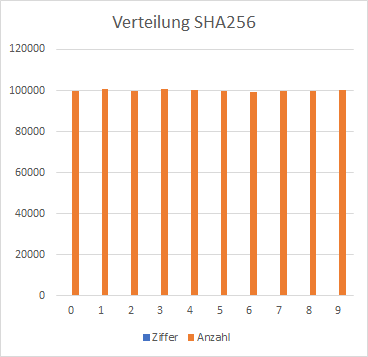
\includegraphics[width=\textwidth]{Figures/verteilung_sha256}
\centering
\decoRule
\captionof{figure}{Verteilung der SHA256 Hashfunktion}
\label{fig:verteilung_sha256}
\end{minipage}


\subsection{Manipulationsversuch durch Miner} \label{btc_eval_miner}
Dieser Abschnitt untersucht ab welchem Einsatzbetrag es für einen Miner profitabel ist, einen gültigen Blockhash zu verwerfen, um den Ausgang des Glücksspiel zu beeinflussen.

Betrachten wir dazu das Bitcoin Netzwerk Anfang Februar 2018. Der Preis pro Bitcoin beträgt 8000 Euro. Der Mining Reward liegt bei 12,5 Bitcoin pro Block\footnote{Dieses Beispiel vernachlässigt die durch das Minen des Blocks erhaltenen Transaktionsgebühren.}. Für das Lösen eines gültigen Blocks erhält ein Miner somit 100000 Euro.
Angenommen ein Miner besitzt eine Hashrate $h$, nimmt an einem Glücksspieltopf mit $n\in\{2, 5, 10\}$ Personen und einem Einsatz von $E$ teil. Mit einer Wahrscheinlichkeit von $h$ findet der Miner den Block für die Gewinnerauswahl und kann entscheiden, ob er den Block veröffentlicht oder verwirft. Mit einer Wahrscheinlichkeit von $1-h$ findet ein anderer Miner des Bitcoin Netzwerks den Block für die Gewinnerauswahl und der Miner kann den Ausgang des Spiels nicht beeinflussen.

Für diese Betrachtung muss der Erwartungswert für beide folgenden Szenario berechnet werden:

\subsubsection{Szenario 1} 
Der Miner findet einen gültigen Block, durch den er das Glücksspiel verliert. Er akzeptiert sein Schicksal und es kommt zu keinem Manipulationsversuch. Der Erwartungswert beträgt $100000 - E$ Euro.
\subsubsection{Szenario 2} 
Der Miner findet einen gültigen Block, durch den er das Glücksspiel verliert. Er verwirft diesen Block und versucht sein Glück erneut um den Ausgang des Glücksspiels zu seinen Gunsten ändern zu können. Da es sich beim Mining um einen gedächtnislosen Prozess handelt, hat der Miner ab diesem Moment erneut eine Wahrscheinlichkeit von $h$ einen gültigen Block zu finden. Für die Berechnung des Erwartungswerts müssen die folgenden Ausgänge berücksichtigt werden:\\
\textbf{1. Fall:} Der Miner findet einen weiteren Block, der das Spiel zu seinen Gunsten entscheidet. Dieser Fall tritt mit einer Wahrscheinlichkeit von $h*\frac{1}{n}$ ein. Der Miner erhält den Blockreward und den Einsatz der Mitspieler: $100000 + (n-1)*E$ Euro.\\
\textbf{2. Fall:} Der Miner findet zwar einen weiteren Block, verliert durch diesen dennoch das Spiel. Dieser Fall tritt mit einer Wahrscheinlichkeit von $h*\frac{n-1}{n}$ ein. In diesem Fall entscheidet er sich den Block einzulösen um den Blockreward zu erhalten. Der Miner erhält somit $100000 - E$ Euro.\footnote{Der Miner könnte den Block erneut verwerfen und versuchen einen weiteren gültigen Block zu finden.}\\
%Die Wahrscheinlichkeit 3 gültige Blöcke hintereinander zu finden beträgt selbst bei einer Hashrate von $h=0,25$ unter 2 Prozent.
\textbf{3. Fall:} Ein anderer Miner findet den nächsten Block, der das Glücksspiel zu Gunsten des Miners entscheidet. Dieser Fall tritt mit einer Wahrscheinlichkeit von $(1-h)*\frac{1}{n}$ ein. Der Miner verliert den Blockreward, gewinnt allerdings das Spiel und erhält somit $(n-1)*E$ Euro.\\
\textbf{4. Fall:} Ein anderer Miner findet den nächsten Block und ein anderer Teilnehmer gewinnt durch diesen das Spiel. Dieser Fall tritt mit einer Wahrscheinlichkeit von $(1-h)*\frac{n-1}{n}$ ein. Der Miner verliert den Blockreward und seinen Einsatz: $-E$ Euro.\\\\
\vspace{0.5cm}
Der Erwartungswert von Szenario 2 berechnet sich zu $ h*100000$ Euro.\footnote{Die Anzahl Teilnehmer des Spiels haben keine Auswirkung auf den Erwartungswert. Die Variable $n$ verschwindet beim Vereinfachen der Erwartungswertgleichung.}\\
%\vspace{0.5cm}
Setzt man die Erwartungswerte beider Szenarien gleich, ergibt sich folgende Gleichung: $100000 - E = h*100000$.\\Formt man diese nach $E$ um, ergibt sich: $E=- h*100000 +10000$.\\
Diese Gleichung gibt an, wie hoch der Einsatz des Spiels sein muss, damit es für einen Miner mit Hashrate $h$ finanziell Sinn macht, das Spiel durch das zurückzuhalten eines gültigen Blocks zu manipulieren.

\begin{table}[H]
\centering
\caption{Profitabilitätsgrenze eines Manipulationsversuchs}
\label{tab:btc_mining_attack}
\begin{tabular}{|c|c|}
\hline
Hashrate (h) & Einsatz (E) \\ \hline
0,05                     & 95000       \\ \hline
0,1                      & 90000       \\ \hline
0,15                     & 85000       \\ \hline
0,2                      & 80000       \\ \hline
0,25                     & 75000       \\ \hline
0,3                      & 70000       \\ \hline
0,35                     & 65000       \\ \hline
0,4                      & 60000       \\ \hline
0,45                     & 55000       \\ \hline
0,5                      & 50000       \\ \hline
\end{tabular}
\end{table}

Aus Tabelle \ref{tab:btc_mining_attack} geht hervor, dass es selbst für einen Miner, der die Hälfte der Hashrate des Bitcoin Netzwerkes kontrolliert, nur profitabel ist gültige Blöcke zu verwerfen, falls der Einsatz des Spiels über 50000 Euro beträgt.

\begin{figure}[H]
\centering
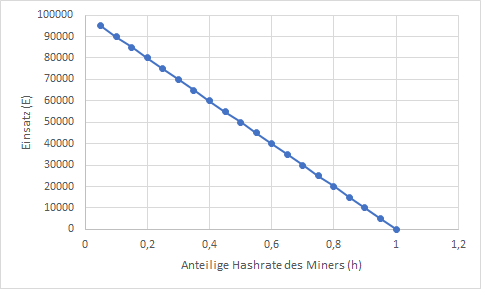
\includegraphics[width=1\linewidth]{Figures/hE}
\decoRule
\caption{}
\label{fig:eH}
\end{figure}


%Die Berechnung des Erwartungswerts gibt eine Aussage ab welchem Einsatz es sich für den Miner lohnt einen gültigen Block zu verwerfen um den Ausgang des Spiels zu manipulieren. Sei $E$ der Einsatz des Topfes. 

%Da der Miner eine Hashrate von 20 Prozent hat, liegt die Wahrscheinlichkeit das der Miner den nächsten Block findet bei 0,2. Falls er den gefundene Blockhash verwirft, da er durch diesen seinen Glücksspieleinsatz verlieren würde, muss er es schaffen vor einem anderen Miner einen weiteren Blockhash zu berechnen. Ansonsten verliert er den Blockreward. Die Wahrscheinlichkeit das der Miner zwei gültige Blockhashs hintereinander findet, liegt bei 0,2 * 0,2 = 0,04 und ist somit verschwindend gering.


Die Hashrate des Bitcoin Netzwerks beträgt circa 30000000 Tera-Hash pro Sekunde (TH/s) \cite{blockchain_info_hashrate}. Einer der profitabelsten Bitcoin ASICs ist der Antminer S9 der Firma Bitmain\footnote{\url{https://www.bitmain.com/}}. Dieser kostet im Einkauf 900 Euro und liefert eine Rechenleistung von 14 TH/s. Ein Miner der ein zwanzigstel($h=0,05$) der Rechenleistung des Bitcoin Netzwerks besitzt, benötigt umgerechnet über 100000 Antminer S9. Somit betragen alleine die Anschaffungskosten der Mining Hardware 90 Millionen Euro.

Bei Proof-of-Work Kryptowährungen wie Bitcoin hat es sich durchgesetzt, dass Miner ihre Rechenleistung in Mining Pools bündeln und gemeinsam nach dem nächsten Block suchen. Findet der Pool einen gültigen Block, wird der Blockreward unter den Teilnehmern des Pools aufgeteilt.

\begin{figure}[H]
\centering
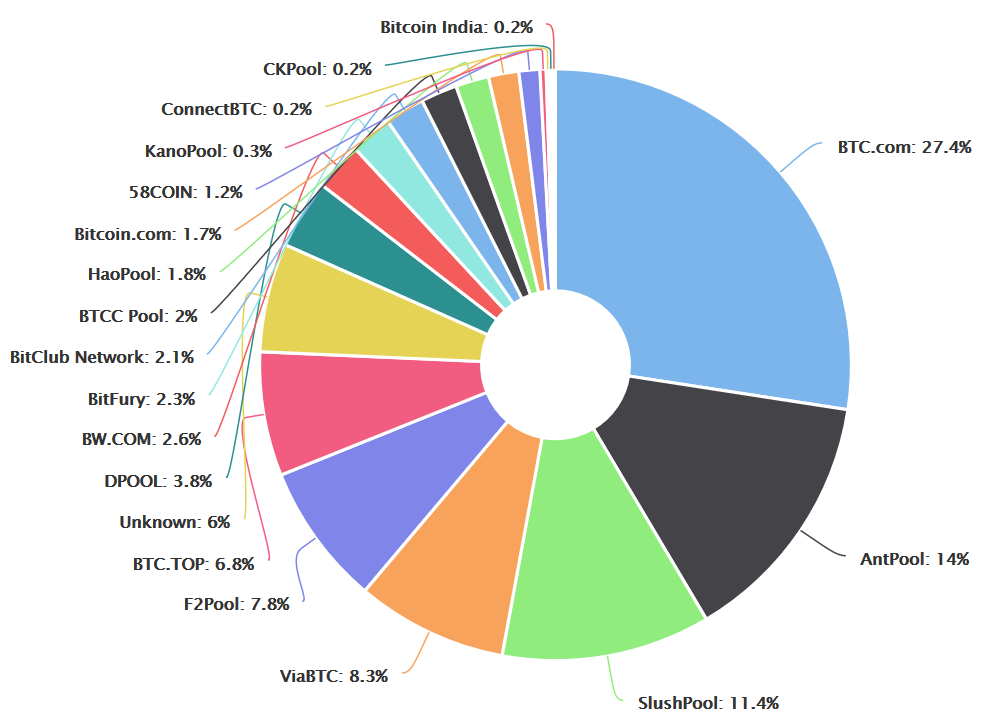
\includegraphics[width=1\linewidth]{Figures/btc_mining_pools}
\decoRule
\caption{Bitcoin Mining Pool Hash Rate \cite{blockchain_info_pools}}
\label{fig:btc_mining_pools}
\end{figure}

Abbildung \ref{fig:btc_mining_pools} zeigt die Verteilung der Hashrate des Bitcoin Netzwerks basierend auf den Blöcken der 4 letzten Tage\footnote{Die Graphik wurde am 10.05.2018 auf Blockchain(dot)Info erstellt. Der Bitcoin Knoten von Blockchain(dot)Info ist mit den aufgelisteten Pools verbunden und schreib einen neuen Block dem Pool zu von dem Blockchain(dot)Info diesen als erstes empfangen hat. Die Statistik ist daher mit Vorsicht zu genießen.} Aus der Grafik geht hervor, dass der größte Pool circa 25\% der Hashrate des Bitcoin Netzwerks besitzt. Hierbei ist es wichtig hervorzuheben, dass sich die eigentliche Mining Hardware im Besitz von Privatpersonen befindet. Diese Privatpersonen können den Mining Pool wechseln, sollten sie nicht mit den Praktiken des Pools einverstanden sein. Ein Pool, der gültige Blöcke nicht an das Bitcoin Netzwerk weiterleiten, da er den Ausgang eines Glücksspiels bestimmen möchte, riskiert damit Marktanteile einzubüßen.

\subsection{Auszahlungstransaktion} \label{sssec:Auszahlungstransaktion}
Die Glücksspielanwendung erzeugt für jede Einzahlung eine eigene Einzahlungsadresse statt für jeden Benutzer die gleiche Adresse zu verwenden. Dies hat den Vorteil, dass die Anwendung dem Benutzer anzeigen kann, dass seine Bitcoin Einzahlung eingegangen ist. Die folgenden Abbildungen betrachten die Auszahlungstransaktion des Beispiels aus Abschnitt \ref{ssec:btc_gui} betrachtet.

\begin{figure}[H]
\centering
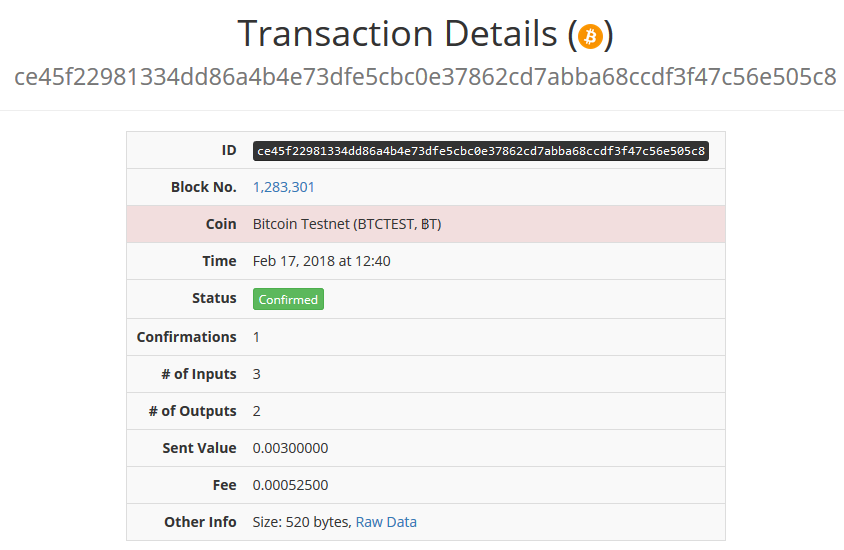
\includegraphics[width=1\linewidth]{Figures/btc_gui/btc_txn}
\decoRule
\caption{Auszahlungstransaktion Details}
\label{fig:btc_txn}
\end{figure}

Abbildung \ref{fig:btc_txn} zeigt in welchen Block die Transaktion aufgenommen wurde, den Status, den Wert, die Transaktionsgebühr und die Größe der Transaktion.
\footnote{Momentan zahlt die Glücksspielanwendung die Auszahlungstransaktionsgebühr aus eigener Tasche. Eigentlich müsste die Transaktionsgebühr von dem Gewinnbetrag abgezogen werden.}

\begin{figure}[H]
\centering
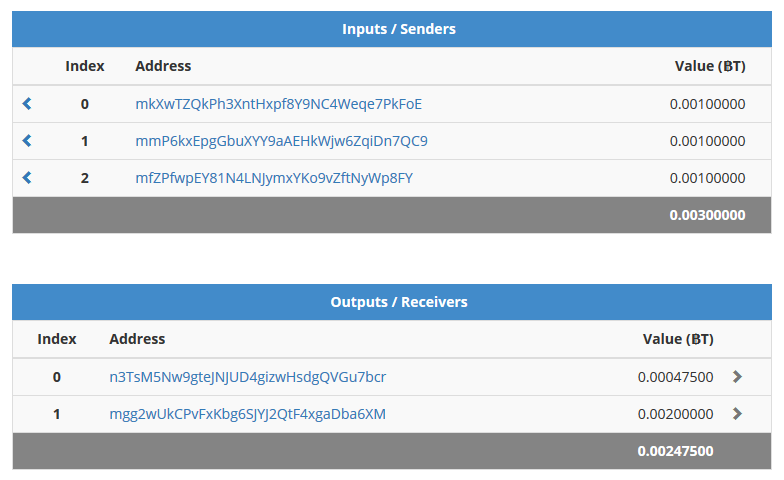
\includegraphics[width=1\linewidth]{Figures/btc_gui/btc_txn_input_output}
\decoRule
\caption{Auszahlungstransaktion Inputs und Outputs}
\label{fig:btc_txn_input_output}
\end{figure}


Abbildung \ref{fig:btc_txn_input_output} zeigt welche Inputs und Outputs für die Transaktion verwendet wurden. Output Adresse 1 gehört der Wallet der Glücksspielanwendung und stellt die Wechselgeldadresse dar.


\begin{figure}[H]
\centering
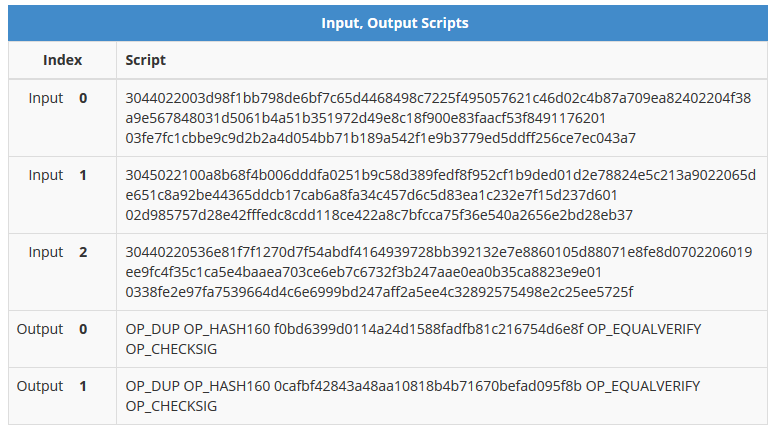
\includegraphics[width=1\linewidth]{Figures/btc_gui/btc_txn_input_output_scripts}
\decoRule
\caption{Auszahlungstransaktion Skripts}
\label{fig:btc_txn_input_output_scripts}
\end{figure}

Die Anwendung muss in der Auszahlungstransaktion für jede Input Adresse eine gültige Signatur angeben, obwohl alle Adressen von der gleichen Wallet kontrolliert werden. Hier könnte in Zukunft die Verwendung sogenannter Schnorr Multi-Signaturen \cite{schnorr_sig} aushelfen. Durch diese lassen sich alle Signaturen der Inputs durch eine einzige Signatur ersetzen.

\subsection{Blockchain Mining Varianz}
Der Begriff Blockchain Mining Varianz beschreibt den Umstand, dass die Miner des Netzwerkes entweder Glück oder Pech bei der Suche nach dem nächsten gültigen Blockhash haben können. Bei Bitcoin gibt es daher nicht genau alle 10 Minuten einen neuen Block, sonder durchschnittlich alle 10 Minuten. Für die Glücksspielanwendung bedeutet dies, dass die Zeit zwischen der letzten Einzahlung und der Auswahl des Gewinners variieren kann. In der Praxis kommt es vor, dass man 30 Minuten und mehr auf den nächsten Block warten muss. Dies ist für den Spieler eine recht lange Zeit. Das Proposal \cite{bobtail} liefert ein Verfahren, das die Blockchain Mining Varianz stark verringert. Dieser Vorschlag ist bisher allerdings noch nicht in den Bitcoin Sourcecode eingeflossen.
Eine andere Möglichkeit die Wartezeit für den Spieler zu verringern ist es eine  Kryptowährung mit einer geringeren Blockzeit zu verwenden. Beispiele hierfür sind LiteCoin mit einer Blockzeit von 2,5 Minuten, die auf Privatsphäre spezialisierte Währung Monero mit einer Blockzeit von 2 Minuten und Ethereum mit einer Blockzeit von 12 Sekunden. Bei einer geringen Blockzeit kommt es häufiger zu sogenannten Blockchain Forks. Weitere Informationen zu den genannten Kryptowährungen sind unter \cite{coin_ltc}, \cite{coin_xmr} und \cite{coin_eth} verfügbar.

\subsection{Blockchain Forks} \label{sssec:btc_fork}
Blockchain Forks entstehen, falls zwei Miner unabhängig voneinander mehr oder weniger gleichzeitig einen validen Block finden. Beide Miner broadcasten ihren Block schnellstmöglich an die Teilnehmer des Peer-to-Peer Netzwerks. Aufgrund von Netzwerkverzögerungen kommt es nun dazu, dass ein Teil des Netzwerks Block 1 und der restliche Teil des Netzwerks Block 2 zuerst enthält. Beide Blockchain-Ketten sind nun gleich lang.
\begin{figure}[H]
\centering
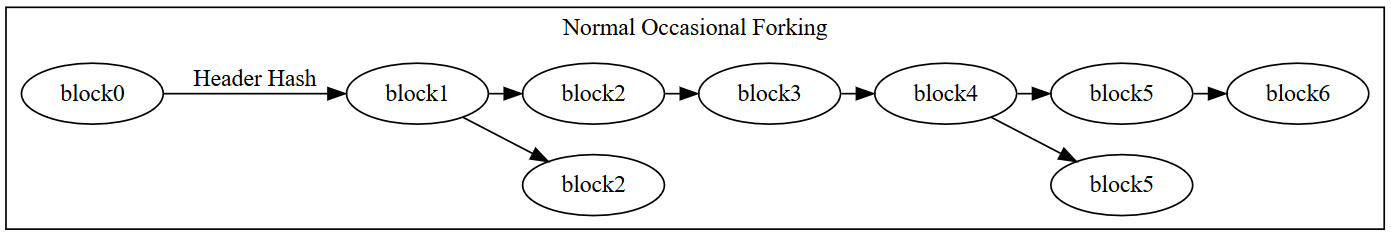
\includegraphics[width=1\linewidth]{Figures/btc/fork_normal}
\decoRule
\caption{Bitcoin Fork}
\label{fig:fork_normal}
\end{figure}
Der nächste gefundene Block entscheidet, auf welche Kette sich das Netzwerk einigt\footnote{Unter der Annahme, dass es nicht erneut zu einem Blockchain Fork kommt.}. Die Bitcoin Konsensregeln legen fest, dass die Teilnehmer des Netzwerks immer der längsten Kette, die somit am meisten Proof-of-Work beinhaltet, folgen. Dies erlaubt es jedem Bitcoin Knoten, ohne Trusted Third Party festzustellen, welche Version der Blockchain die echte ist. Forks kommen bei Bitcoin durch die hohe Hashrate des Netzwerks und die somit sehr hohe Difficulty recht selten vor. \cite{orphaned-blocks} zeigt an, wie oft gültige Blöcke gefunden und nicht Teil der längsten Blockchain werden.

\subsection{Betrugsmöglichkeiten}

Dieser Abschnitt betrachtet in wie weit die Glücksspielanwendung potentielle Spieler betrügen kann, sollte sie gehackt und zu ausschließlich diesem Zweck modifiziert werden.
Die Anwendung hat die volle Kontrolle darüber welche Ausgabe sie dem Benutzer anzeigt. Sie hat allerdings keine Kontrolle über den Status der Blockchain. 

Die Anwendung könnte beispielsweise anzeigen, dass der Topf nach der Einzahlung durch einen Spieler immer noch leer ist. Die Transaktion auf die Einzahlungsadresse existiert dann zwar in der Blockchain allerdings reagiert die Anwendung nicht entsprechend. Dies hat zur Folge, dass jeder Spieler der eine Einzahlung tätigt, sein Geld verliert. Allerdings merkt der Benutzer dies und kann somit eine weitere Verwendung der Anwendung unterlassen. Ein solch plumper Manipulationsversuch fällt somit direkt auf.

Ein weitere Betrugsmöglichkeit ist, dass die Glücksspielanwendung sich bis zur Gewinnerauswahl korrekt verhält, dann allerdings keine Auszahlung tätigt. Alle einzahlenden Spieler merken den Betrug, verlieren aber dennoch ihr Geld.

Bei beiden vorgestellten Betrugsversuchen fällt der Betrug immer mindestens einem Spieler auf. Die Verwendung einer solchen Anwendung macht nur Sinn, falls man den Betreiber des Services kennt und diesen im Zweifel juristisch haftbar machen kann.\\
Das folgende Kapitel betrachtet wie sogenannte Smart Contracts dieses Problem lösen. Ein Smart Contract erlauben es die Geschäftslogik der Glücksspielanwendung in die Blockchain zu schreiben. Die Geschäftslogik wird somit nicht mehr von der Anwendung, sondern von jedem Teilnehmer des Peer-to-Peer Netzwerks ausgeführt. 


\chapter{Zweiter Ansatz: Ethereum} % Main chapter title

\label{eth} % For referencing the chapter elsewhere, use \ref{eth} 

\section{Grundlagen}
Ethereum ist genau wie Bitcoin ein Peer-to-Peer Netzwerk Protokoll, dass auf einer öffentlichen Blockchain basiert und einen Systemzustand verwaltet. Es handelt sich im Gegensatz zu Bitcoin um eine generalisierte Blockchain die nicht nur Finanztransaktionen speichern kann, sondern sogenannte Smart Contracts\footnote{Bitcoin Transaktionen beinhalten im Grunde auch Smart Contracts allerdings sind diese weniger Mächtig. Abschnitt \ref{eth_grundlagen_btc_diff} geht genauer auf die Unterschiede zwischen Bitcoin und Ethereum ein.}. Ethereum sieht sich als eine Open Source Plattform, die es ermöglicht dezentrale Applikationen zu entwickeln und bereitzustellen.

\subsection{Smart Contracts}
Ethereum ermöglicht es Geschäftsprozesse in Form von Smart Contracts zu programmieren und von einem globalen dezentralen Netzwerk ausführen zu lassen. Ein Contract ist ein Programm bestehend aus einer Reihe von Anweisungen, die ausgeführt werden, sobald das Programm eine Nachricht in Form einer Transaktion erhält. Contracts haben die Möglichkeit Daten aus der Blockchain auszulesen und auf ihr Daten zu speichern. Smart Contracts können sowohl von Menschen als auch von anderen Contracts ausgelöst werden. Contracts können daher mit anderen Contracts über die vom Programmierer festgelegte Schnittstelle interagieren. Es handelt sich bei einem Smart Contract also nicht um einen Vertrag, der erfüllt werden muss, sondern um ein öffentliches Stück Software, dass den Zustand eines Ethereum Accounts verwaltet.
\subsection{Ethereum Accounts}
Um Ethereum nutzen zu können braucht man einen Account. Ethereum Accounts bestehen aus:\\
\begin{itemize}
\item Einer 20 Byte langen Adresse,
\item einem Kontostand in Ether(siehe Abschnitt \ref{eth_ether}),
\item einem Nonce-Wert der sicherstellt, dass Transaktionen nur einmal ausgeführt werden können,
\item Smart Contract Code (optional),
\item und Speicherplatz (optional).
\end{itemize} In Ethereum gibt es zwei Arten von Accounts. Die erste Art ist eine Adresse, die, wie bei Bitcoin, durch den Besitz des privaten Schlüssels kontrolliert wird. Diese Art von Account wird durch eine Wallet Software verwaltet. Die zweite Art ist ein  Contract Account, der durch den Smart Contract Code kontrolliert wird. Der Smart Contract Code verwaltet eigenständig den Kontostand des Accounts und verhält sich genau so, wie der Programmierer es festgelegt hat.

\subsection{Transaktionen}
Interaktionen mit dem Ethereum Netzwerk finden in Form sogenannter Transaktionen statt. Transaktionen sind, durch den privaten Schlüssel eines Ethereum Account, signierte Datenpakete, die eine Nachricht(siehe Abschnitt \ref{eth_messages}) beinhalten. Transaktionen beinhalten:
\begin{itemize}
\item den Empfänger der Nachricht,
\item eine digitale Signatur, die den Absender der Nachricht identifiziert,
\item eine Anzahl an Ether, die an den Empfänger versandt wird,
\item Daten (Bytes), die vom Contract ausgelesen werden können (optional),
\item einen sogenannten Gas-Wert, der die maximale Anzahl Rechenschritte festlegt, die die Transaktion bei der Ausführung nutzen darf
\item und den GAS-Preis, der festlegt, wie viel der Absender bereit ist für die Ausführung eines Rechenschritts der Transaktion zu zahlen.
\end{itemize}

Es gibt zwei verschiedene Arten von Transaktion. Sie unterscheiden sich durch die in der Transaktion angegebene Empfangsadresse. 
Wird die Empfangsadresse durch einen privaten Schlüssel kontrolliert, handelt es sich lediglich um eine Finanztransaktion, die Ether vom Sender zum Empfänger Account transferiert. Anderenfalls handelt es sich um eine Transaktion, die den Contract Code der Empfangsadresse ausführt. Welche Funktion ausgeführt werden soll, wird vom Sender im Datenfeld der Transaktion kodiert.

\subsection{Nachrichten}\label{eth_messages}
Bei Nachrichten handelt es sich um virtuelle Objekte, die im Gegensatz zu Transaktionen nicht abgespeichert werden, sondern lediglich in der Ethereum Virtual Machine (siehe Abschnitt \ref{eth_evm}) verwendet werden. \if lediglich zur Interaktion mit dem Contract Code eines Smart Contracts verwendet werden.\fi Ein weiterer Unterschied ist, dass Transaktionen im Gegensatz zu Nachrichten immer von ''außen'' erzeugt werden. Nachrichten können hingegen auch von Smart Contracts erzeugt werden. Nachrichten bestehen aus einem impliziten Sender, einem Empfänger, einem Ether-Betrag, einem Gas-Wert und einem optionalen Datenfeld. Genau wie bei Transaktionen führt das versenden von Nachrichten zu der Ausführung des Conrtact Codes der Empfangsadresse.

\subsection{Ether}\label{eth_ether} 
Ether ist die Kryptowährung des Ethereum Netzwerks. Sie entsteht wie bei Bitcoin durch Mining und wird benutzt, um für Transaktionsgebühren und die Ausführung von Contract Code zu bezahlen. Die kleinste Einheit der Ethereum Währung nennt sich WEI. Ein Ether entspricht $10^{18}$ WEI. Ether bildet durch die Zuhilfenahme des Gas-Werts und Gas-Preis den anti Spam Schutz des Ethereum Netzwerks.
\subsubsection{Gas-Wert}
Da Smart Contracts Schleifen beinhalten und andere Smart Contracts durch Nachrichten aufrufen können, muss sichergestellt werden, dass die Ausführung terminiert. Da es für den Sender der Transaktion schwierig, in manchen Fällen sogar unmöglich\footnote{Beispielsweise wenn der nächste Block eine Transaktion enthält, die bewirkt, dass die eigentlichen Transaktion ein unterschiedlicher Code-Pfad durchlaufen wird.} ist, die Anzahlt Schritte der Ausführung im Vorhinein zu wissen, legt der Absender durch den Gas-Wert die maximale Anzahl Rechenschritte fest, die die Transaktion bei der Ausführung dauern darf.
\subsubsection{Gas-Preis}
Durch den Gas-Preis gibt der Sender einer Transaktion an, wie viel Ether er pro Rechenschritt bereit ist zu bezahlen. Die Ausführung einer Transaktion kann einen Ethereum Account somit um maximal \code{Gas-Wert * Gas-Preis} Ether belasten.

\subsection{Ethereum Virtual Machine}\label{eth_evm} 
In der Ethereum Virtual Machine wird der Smart Contract Code ausgeführt. Sie arbeitet die Anweisungen des Contracts der Reihe nach ab und bricht ab, falls der Gas-Wert nicht für die Ausführung der Transaktion ausreicht. Durch das sequenzielle Abarbeiten der Transaktionen eines Blocks wird der Systemzustand nach und nach von der Ethereum Virtual Machine angepasst.
\begin{figure}[H]
\centering
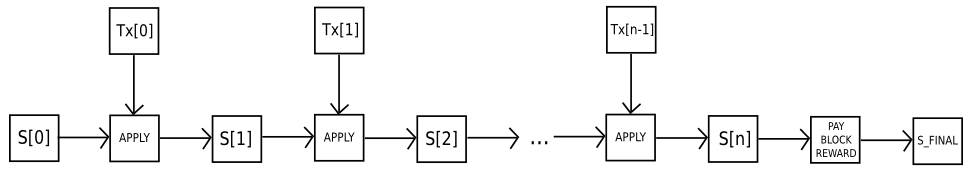
\includegraphics[width=1\linewidth]{Figures/eth/ETH_txn_statetransformation}
\decoRule
\caption{Veränderung des Systemzustand}
\label{fig:ETH_txn_statetransformation}
\end{figure}
Der Systemzustand wird bei Ethereum durch den Zustand aller Ethereum Accounts beschrieben. 

\subsection{Systemzustand Übergangsfunktion}
Die Ethereum Virtual Machine geht bei der Abarbeitung einer Transaktion folgendermaßen vor:
\begin{enumerate}
\item Sie prüft ob die Transaktion gemäß der Konsensregeln korrekt formatiert ist, eine valide Signatur besitzt und ob der Nonce-Wert der Transaktion mit dem Nonce-Wert des Absender-Accounts übereinstimmt. Ist eine dieser Vorbedingungen nicht erfüllt, wird die Bearbeitung der Transaktion abgebrochen. 
\item Es wird die maximal fällige Transaktionsgebühr durch das Multiplizieren des Gas-Werts mit dem Gas-Preis berechnet. Anschließend wird geprüft, ob der Account des Senders genug Ether besitzt, um die berechnete Transaktionsgebühr zu bezahlen. Ist dies der Fall wird die maximale Transaktionsgebühr vom Sender-Account abgezogen. Anderenfalls wird die Bearbeitung der Transaktion abgebrochen. 
\item Nun wird der Gas-Wert der Transaktion um einen gewissen Betrag jedes Transaktionsbyte verringert. Der Sender zahlt auf diese Weise für den Platz, den die Transaktion in der Blockchain einnimmt.
\item Der Ether Wert der Transaktion wird vom Sender auf den Empfänger Account überwiesen. Falls der Empfänger Account noch nicht existiert wird er angelegt. Wird der Empfänger Account durch einen Smart Contract verwaltet, wird der Contract Code entweder vollständig ausgeführt oder aufgrund fehlenden Gas abgebrochen. 
\item Falls der Sender nicht genug Ether oder verbleibendes Gas für die Überweisung besitzt, werden alle bisherigen Veränderungen des Systemzustands rückgängig gemacht. In diesem Fall wird ausschließlich die Transaktionsgebühr  auf den Account des Miners überschrieben.
\item Im erfolgreichen Fall werden die Gebühren des verbleibenden Gas an den Sender zurückerstattet und die Gebühren des verbrauchten Gas an den Account des Miners überschrieben.
\end{enumerate}

\subsection{Systemzustand Beispiel}
Das folgende Beispiel betrachtet, wie das Anwenden eine Transaktion einen alten Systemzustand in einen neuen Systemzustand überführt. 
\begin{figure}[H]
\centering
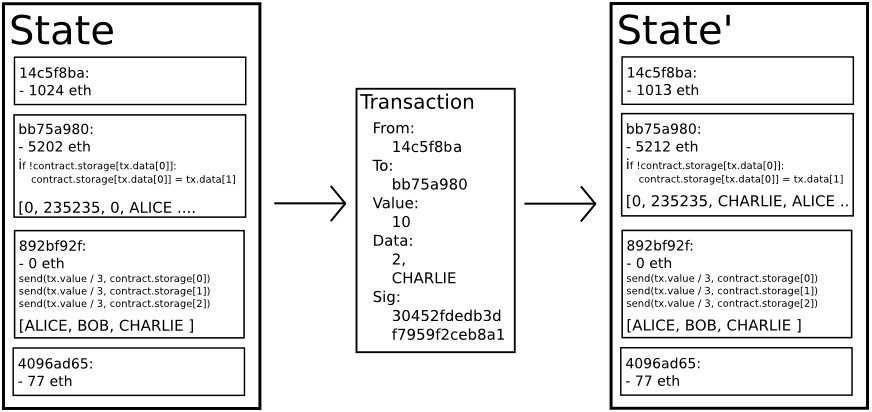
\includegraphics[width=1\linewidth]{Figures/eth/ETH_statetransition_example}
\decoRule
\caption{Veränderung des Systemzustand}
\label{fig:ETH_statetransition_example}
\end{figure}
Die in Abbildung \ref{fig:ETH_statetransition_example} betrachtete Transaktion ruft den Smart Contract des Accounts der Adresse \code{bb75a980} auf. Angenommen die Transaktion überweist einen Betrag von 10 Ether, besitzt einen Gas-Wert von 2000, einen Gas-Preis von 0,001 Ether, enthält 64 Bytes an Daten(\code{data[0]=2,data[1]='CHARLIE'}) und besitzt eine Gesamtgröße von 170 Bytes. Dann erfolgt die Abarbeitung der Transaktion folgendermaßen:
\begin{enumerate}
\item Es wird durch die Prüfung der Signatur einerseits sichergestellt, dass die Daten der Transaktion nicht manipuliert wurden und andererseits, dass die Überweisung der 10 Ether vom Besitzer des Accounts \code{14c5f88a} autorisiert wurde. 
\item Da der Account des Senders über \code{2000 * 0,001 = 2} Ether besitzt, wird die Bearbeitung der Transaktion fortgesetzt und die 2 Ether vom Account des Senders abgezogen.
\item Unter der Annahme, dass man 5 Gas pro Transaktionsbyte bezahlen muss, wird der Gas-Wert von 2000 auf 1150 Gas verringert. (170 Bytes * 5 = 850 Gas) 
\item Der Transaktionsbetrag von 10 Ether wird vom Sender Account \code{14c5f88a} auf den Account \code{bb75a980} überwiesen.
\item Nun wird der Conract Code des Empfängeraccounts ausgeführt:\\ \code{if !contract.storage[tx.data[0]]: contract.storage[tx.data[0]] = tx.data[1]}\\
Da der Speicherplatz des Contracts an Stelle 2 noch nicht verwendet ist, wird  der Wert \code{CARLIE} aus den Transaktionsdaten abgespeichert. Unter der Annahme, dass diese Operationen 150 Gas verbrauchen ergibt sich ein verbleibender Gas-Wert von \code{1150 -150 = 1000}. 
\item Die verbleibenden \code{1000 * 0,001 = 1} Ether werden auf den Account des Senders zurücküberwiesen und die Anpassung des Systemzustands ist fertig\footnote{Im resultierenden Systemzustand aus Abbildung \ref{fig:ETH_statetransition_example} fehlt die an den Miner gezahlte Transaktionsgebühr von 1 Ether. Diese zahlt sich der Miner wie in Abbildung \ref{fig:ETH_txn_statetransformation} gezeigt in der letzten Transaktion zusammen mit den restlichen Transaktionsgebühren des Blocks aus.}.
\end{enumerate}

\subsection{Unterschiede zu Bitcoin}\label{eth_grundlagen_btc_diff} 
\subsubsection{Turing-Vollständigkeit}
Bitcoin besitzt intern auch eine Skript-Sprache zur Ausführung von Transaktionen. Diese ist im Gegensatz zu Ethereum bewusst eingeschränkt und nicht turingmächtig. Da man keine Schleifen programmieren kann, führt dies dazu, dass man Code mehrfach wiederholen muss. Dies führt dazu, dass Transaktionen die Smart Contracts ausdrücken in Bitcoin mehr Platz in der Blockchain einnehmen. Ethereum muss sich aufgrund der Turing-Vollständigkeit um das Halteproblem kümmern. Durch die Angabe eines maximalen Gas-Werts stellt Ethereum sicher, dass die Ausführung einer Transaktion spätestens nach einer gewissen Zeit abgebrochen wird. 
\subsubsection{Betrags-Blindheit}
Der Betrag, der einer Bitcoin-Adresse zugeschrieben wird, kann entweder nur ganz oder gar nicht ausgegeben werden. Dies ist bei Ethereum nicht der Fall. Der Nonce-Wert des Ethereum Accounts verhindert, dass eine Transaktion nicht zweimal ausgeführt werden kann.
\subsubsection{Blockchain-Blindheit}
In Bitcoin kann man bei der Ausführung der Transaktionen nicht auf Blockchain Daten wie Beispielsweise vorherige Blockhash-Werte, Zeitstempel oder None-Werte zugreifen. Eine Transaktion, die einen vorherigen Blockhash ausließt und als Zufallsquelle verwendet ist mit der Bitcoin Skript-Sprache nicht möglich.
\subsubsection{Fehlender Zustand}
Die Ethereum Accounts ermöglichen es einen weitaus komplexeren Systemzustand abzubilden. Bei Bitcoin besteht der Systemzustand lediglich aus der Menge aller Adressen, die Bitcoins besitzen.
\section{Konzept} \label{eth_konzept}

Der Ablauf des Spiels ist mit dem Ablauf aus dem Bitcoin Kapitels nahezu identisch. Die Unterschiede sind, dass das gesamte Spiel vom Nutzer initiiert wird und die Glücksspielanwendung ausschließlich den Spielstatus anzeigt. Dies führt dazu, dass die Spieler keinerlei Vertrauen in die Glücksspielanwendung setzen müssen. Statt aufgrund leichter Überprüfbarkeit die letzte numerische Stelle des Blockhashs für die Gewinnerauswahl zu nutzen, kann bei Ethereum der gesamten Blockhash zur Gewinnerauswahl genutzt werden. Der Spieler kann aufgrund der Konsensregeln darauf vertrauen, dass das Ethereum Netzwerk die Ausführung des Contract Codes korrekt durchführt und die modulo Funktion zur Gewinnerauswahl korrekt berechnet. Die Nutzung des gesamten Blockhashs als Zufallsquelle ermöglicht Töpfe beliebiger Größe. 
Der Ablauf des Spiels lässt sich durch den folgenden Zustandsautomat beschreiben.

\begin{figure}[H]
\centering
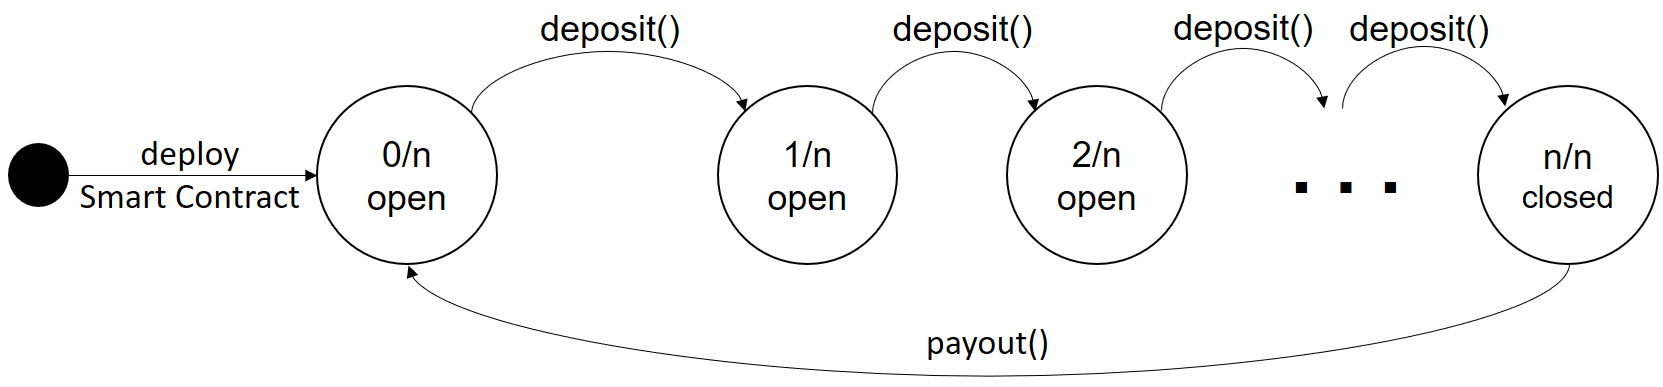
\includegraphics[width=1\linewidth]{Figures/umsetzung_eth/smart_contract_automat_idea}
\decoRule
\caption{Smart Contract Automat}
\label{fig:smart_contract_automat_idea}
\end{figure}

Durch den Aufruf der \code{deploy} Funktion wir der Smart Contract in einer Transaktion an das Netzwerk gesendet und in die Blockchain aufgenommen. Innerhalb des Smart Contracts sind der Einzahlungsbetrag und die Anzahl Teilnehmer \code{n} fest definiert. Ab diesem Moment kann der Code des Smart Contract nicht mehr verändert werden. Im initialen Zustand ist der Topf leer, da noch kein Spieler eingezahlt hat. Nun können genau \code{n} Einzahlungen von Spielern durch den Aufruf der \code{deposit} Funktion getätigt werden. Dazu benötigen die Spieler lediglich einen Ethereum Client, ausreichend Ether\footnote{Einzahlungsbetrags plus Transaktionskosten und optimaler Weise genug Ether für das Bezahlen der \code{payout} Funktion.} und die Adresse des Smart Contracts. Ab dem Zeitpunkt an dem der Smart Contract die letzte Einzahlungstransaktion empfängt, wird der Topf geschlossen und die Blocknummer für die Gewinnerauswahl festgelegt. Der Block der den Gewinner des Topfs entscheidet, muss in der Zukunft liegen und darf nicht vorher bekannt sein, da sonst Betrugsmöglichkeiten entstehen. Zum Zeitpunkt der letzten Einzahlungstransaktion ist es nicht möglich aus dem Smart Contract Code heraus auf den Blockhash des Blocks zuzugreifen in dem sich die letzte Einzahlungstransaktion befindet. Dies liegt daran, dass die Miner das Resultat der Zustandsveränderung aller Transaktionen des Blockes in den Blockheader schreiben müssen und erst anschließend den Blockhash berechnen. Die Transaktionen, die den Contract Code ausführen, können somit nicht auf den Blockhash zugreifen, da dieser zum Zeitpunkt der Codeausführung noch nicht feststeht. Es ist somit unumgänglich nach der letzten Einzahlungstransaktion eine Funktion aufzurufen, die den Gewinner auswählt, die Auszahlung startet und den Topf anschließend für ein neues Spiel wieder öffnet. Dies ist die in Abbildung \ref{fig:smart_contract_automat_idea} gezeigte \code{payout} Funktion.  
\section{Umsetzung}
\subsection{Überblick}
Genau wie bei Bitcoin besteht die Möglichkeit die Glücksspielanwendung entweder direkt mithilfe eines \textit{Light-Nodes} oder indirekt über einen \textit{Full-Node} mit dem Ethereum Netzwerk kommunizieren zu lassen. Für den Ethereum-Teil dieser Masterarbeit findet die Kommunikation indirekt über einen Full-Node statt. Dies ist in Abbildung \ref{fig:eth_anwendung_aufbau} verdeutlicht. Der Full-Node empfängt Transaktionen und Blöcke, validiert diese und akualisiert kontinuierlich den Zustand der, durch die Transaktionen veränderten, Ethereum Accounts. Über die RPC Schnittstelle stellt er diese Daten nach außen bereit. Die Java Bibliothek Web3J \cite{web3j} erleichtert den Aufruf der RPC Schnittstelle des Full Nodes. Anders als bei Bitcoin benötigt die Glücksspielanwendung keine eigene Datenbank, da der Zustand des aktuellen Topfs im Smart Contract und somit ''in der Blockchain'' gespeichert ist.
\begin{figure}[H]
\centering
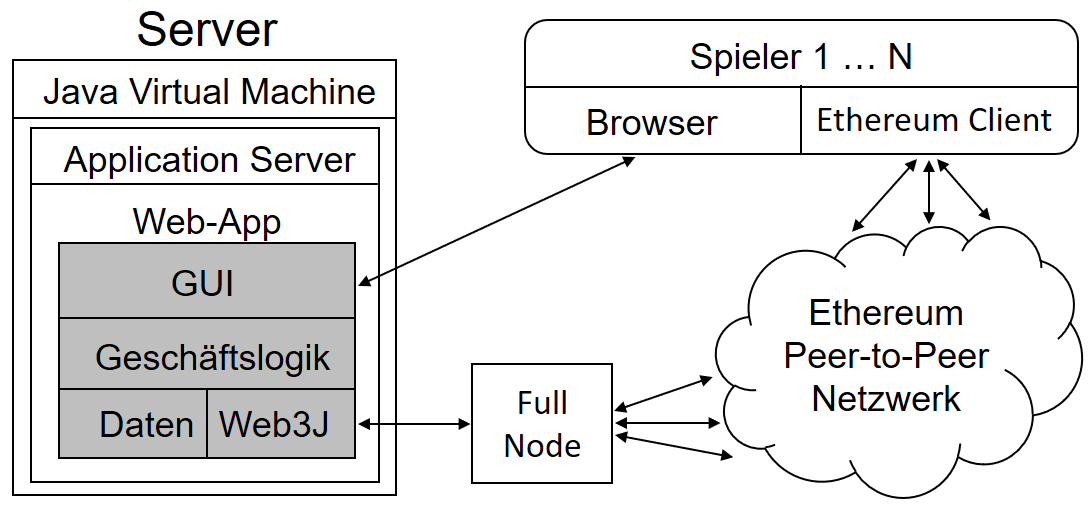
\includegraphics[width=1\linewidth]{Figures/umsetzung_eth/anwendung_aufbau}
\decoRule
\caption{Ethereum: Netzwerk Integration}
\label{fig:eth_anwendung_aufbau}
\end{figure}

Möchte man eine Anwendung direkt in das Ethereum Netzwerk integrieren, bietet sich die Java Bibliothek \code{EthereumJ} \cite{ethereumj} an. 

\subsection{Smart Contract}\label{eth_smart_contract}
Die folgenden Codestücke beschreiben den \code{TrustlessGambling} Smart Contract in der Programmiersprache Solidity. Dokumentation zur Solidity Programmiersprache findet man unter \cite{doc_solidity}.

\subsubsection{Datenmodell}
Das folgende Codestück zeigt den Rahmen, alle Variablen und den Konstruktor des Smart Contracts.
\begin{lstlisting}[basicstyle=\small]
pragma solidity ^0.4.0;
contract TrustlessGambling {
    // constants
    uint8 public constant NBR_OF_SLOTS =3;
    uint public constant EXPECTED_POT_AMOUNT=1000;// WEI
    uint8 public constant PAYOUT_BLOCK_OFFSET =1;    
    // pot values
    uint public nbrOfParticipants;
    address[NBR_OF_SLOTS] public depositAddresses;
    address[NBR_OF_SLOTS] public payoutAddresses;
    uint public closingBlockNumber;
    uint public payoutBlockNumber;
    bytes32 public payoutBlockHash;
    uint public winner; // 0 -> NBR_OF_SLOTS-1
    bool public potClosed;
    uint public nbrOfMissedPayouts;
    // constructor
    function TrustlessGambling() public {
        nbrOfParticipants = 0;
        potClosed = false;
        nbrOfMissedPayouts = 0;
    }
}
\end{lstlisting}


Zeile 1 definiert in welcher Solidity-Version der Smart Contract geschrieben ist. Dies muss vom Compiler bei der Übersetzung zu Bytecode berücksichtigt werden. Zeile 2 legt den Namen des Smart Contracts fest. Über die beiden Konstanten in Zeile 4 und 5 kann man die Anzahl Spieler und den von jedem Spieler erwarteten Einzahlungsbetrag festlegen. Die in Zeile 6 definierte Konstante legt fest, welcher Block (ab der letzten Einzahlungstransaktion) den Gewinner bestimmt. Diese Werte können nach der Bereitstellung des Smart Contracts nicht mehr verändert werden. Die Variablen von Zeile 8 bis Zeile 16 werden vom Smart Contract manipuliert und speichern den Zustand des aktuellen Topfs. Zeile 8 speichert wie viele Teilnehmer bereits eingezahlt haben. Zeile 9 und 10 speichern die Ein- und Auszahlungsadressen\footnote{Die Einzahlungsadressen werden nur zur Anzeige für die GUI-Anwendung abgespeichert und sind für das eigentliche Spiel irrelevant. Das Weglassen dieser Adressen würde zu günstigeren Transaktionskosten für Einzahlungstransaktionen führen.} der aktuellen Teilnehmer. Die Zeilen 11 bis 14 speichern alle für die Gewinnerauswahl benötigten Werte. Zeile 15 definiert über den Wahrheitswert \code{potClosed}, ob der Topf offen ist und Einzahlungen stattfinden können. Der Nutzen des Wertes aus Zeile 16 wird im Rahmen des \textbf{Auszahlungen} Abschnitts erklärt. Zeile 18 bis 22 beinhalten den einmalig bei der Bereitstellung des Smart Contracts aufgerufenen Konstruktor. Alle Variablen des Smart Contracts sind zur Schaffung maximaler Transparenz mit dem Schlüsselwort \code{public} markiert. Dies erlaubt es den Nutzern alle Werte des Smart Contract abzurufen.

\subsubsection{Einzahlungen}
Einzahlungen finden über die beiden \code{deposit} Methoden statt. Diese sind mit dem Schlüsselwort \code{payable} markiert. Dies bedeutet, dass Transaktionen einen Ether-Betrag beim Aufruf dieser Methoden angeben können.
\begin{lstlisting}
function deposit() payable public {
    deposit(msg.sender);
}
function deposit(address _payout) payable public {
    assert(msg.value == EXPECTED_POT_AMOUNT);
    assert(!potClosed);
    depositAddresses[nbrOfParticipants] = msg.sender;
    payoutAddresses[nbrOfParticipants] = _payout;
    nbrOfParticipants++;
    if (nbrOfParticipants == NBR_OF_SLOTS){
        closingBlockNumber = block.number;
        payoutBlockNumber = closingBlockNumber + PAYOUT_BLOCK_OFFSET;
        potClosed = true;
    }
}
\end{lstlisting}


Nutzt der Spieler die Methode aus Zeile 1 wird als Auszahlungsadresse einfach die Adresse der Transaktion verwendet. Nutzt der Spieler die Methode aus Zeile 4 hat er die Möglichkeit eine beliebige Auszahlungsadresse anzugeben. Bei der Einzahlung wird zunächst in Zeile 5 geprüft, ob der Topf offen ist. Ist dies der Fall prüft Zeile 6, dass der Transaktionsbetrag mit dem erwarteten Einzahlungsbetrag übereinstimmt. Anschließend wird die Ein- und Auszahlungsadresse abgespeichert und die aktuelle Anzahl Teilnehmer um eins erhöht. Zeile 10 prüft, ob es sich um die letzte Einzahlungstransaktion handelt und schließt gegebenenfalls den Topf. Vor dem Schließen des Topfs wird in Zeile 11 die aktuelle Blocknummer abgespeichert und anschließend die Blocknummer für die Gewinnerauswahl berechnet.

\subsubsection{Auszahlungen}\label{sssec:eth_nbrOfMissedPayouts}
Auszahlungen finden durch den Aufruf der \code{payout} Methode statt. Diese ist nicht mit dem Schlüsselwort \code{payable} markiert und erwartet keinen Ether-Betrag beim Aufruf.
\begin{lstlisting}[basicstyle=\small]
function payout() public{
    assert(potClosed);
    assert(block.number>payoutBlockNumber);
    payoutBlockHash = block.blockhash(payoutBlockNumber); 
    if(payoutBlockHash == 0){
        nbrOfMissedPayouts++;
    }else{
        winner = uint256(payoutBlockHash) % NBR_OF_SLOTS;
        address winnerAddress = payoutAddresses[winner];
        uint amount= EXPECTED_POT_AMOUNT*NBR_OF_SLOTS;
        amount += EXPECTED_POT_AMOUNT*NBR_OF_SLOTS*nbrOfMissedPayouts;
        winnerAddress.transfer(amount); // send pot amount to winner
        nbrOfMissedPayouts = 0;
    }
    potClosed = false;
    nbrOfParticipants=0;
}
\end{lstlisting}


Die Methode kann nur aufgerufen werden, falls der Topf geschlossen ist und die aktuelle Blocknummer bereits höher als die Blocknummer für die Gewinnerauswahl ist. Sind diese Bedingungen erfüllt, hängt der weitere Verlauf der Abarbeitung der \code{payout} Methode vom Zeitpunkt des Methodenaufrufs ab. Smart Contracts können laut einer Konvention bei ihrer Ausführung nur auf die Werte der 256 letzten Blockheader zugreifen (siehe \cite{doc_solidity_global_var}). Wenn der in Zeile 4 angefragte \code{payoutBlockHash} älter als 256 Blöcke ist, gibt \code{block.blockhash(<number>)} den Wert 0 zurück und Fall 1 tritt ein.
\begin{enumerate}
\item Fall (Zeile 5): Der Aufruf der \code{payout} Methode findet zu spät statt. Es kommt zu keiner Auszahlung, da der Smart Contract nicht auf den entscheidenden Blockhash zugreifen kann. Der Smart Contract erhöht die \code{nbrOfMissedPayouts} Variable um eins. Dies führt dazu, dass der Betrag des Topfs in den nächsten Topf verschoben wird. 
\item Fall (Zeile 8): Der Aufruf der \code{payout} Methode findet rechtzeitig statt. Der Smart Contract berechnet den Gewinner indem er den Blockhash zu einem Integer castet und diese sehr hohe Zahl modulo der Anzahl Teilnehmer rechnet. Anschließend wird der korrekte Auszahlungsbetrag berechnet und in Zeile 12 an die Auszahlungsadresse des Gewinners versandt.
\end{enumerate}
Zum Schluss wird der Topf wieder geöffnet (Zeile 15) und die Anzahl der teilnehmenden Spieler auf 0 gesetzt (Zeile 16).

\subsection{Smart Contract Bereitstellung}
Nachdem man den Smart Contract programmiert hat, muss man ihn zu Bytecode kompilieren und anschließend in einer Transaktion an das Ethereum Netzwerk senden. Der in Solidity geschriebene Contract Code kann mithilfe eines Online-Compilers \footnote{\url{http://remix.ethereum.org}} kompiliert werden. Das Kompilieren erzeugt die Dateien \code{Trustless-} \code{Gambling.bin} und \code{TrustlessGambling.abi}. Diese enthalten den Bytecode und das Smart Contract \textbf{A}pplication \textbf{B}inary \textbf{I}nterface.
Um in der Programmiersprache Java mit dem Smart Contract interagieren zu können, stellt Web3J sogenannte Comandline Tools zur Verfügung. Durch den Aufruf des folgenden Befehl wird die Java Klasse \code{TrustlessGambling} generiert:
\begin{verbatim}
web3j solidity generate TrustlessGambling.bin TrustlessGambling.abi
 -o /path/to/src/main/java -p com.ossel.gamble.ethereum.generated
\end{verbatim}
Da zur Bereitstellung des Smart Contracts auch die entsprechende Transaktionsgebühr gezahlt werden muss, wird eine Wallet benötigt. Web3J hilft auch bei diesem Schritt. Der folgende Befehl leitet die Generierung einer Wallet ein:
\begin{verbatim}
web3j wallet create
\end{verbatim}
Über die Kommandozeile muss der Benutzer den gewünschten Wallet-Dateinamen  und ein Passwort angeben. In diesem Beispiel wird der Dateiname \textit{ethereum.json} und das Passwort \textit{changeit} verwendet. Anschließend wird die Wallet generiert und die Ethereum Account Adresse ausgegeben. Eine genaue Beschreibung der Web3j Commandline Tool Befehle findet man unter \cite{web3j_clt}.
Bevor der Smart Contract durch eine Transaktion veröffentlicht wird, muss zunächst eins der folgenden Ethereum Netzwerke gewählt werden:
\begin{enumerate}
\item Mainnet: Genau wie bei Bitcoin handelt es sich bei diesem Netzwerk um das Hauptnetzwerk. 
\item Ropsten Testnetz: Hierbei handelt es sich um ein Testnetz, das Proof-of-Work als Konsensalgorithmus verwendet. Es ist dem Ethereum Mainnet am ähnlichsten. Der auf diesem Netzwerk ausgetauschten Ether-Währung wird allerdings kein finanzieller Wert zugemessen.
\item Rinkeby Testnetz: Hierbei handelt es sich um ein Testnetz, das nicht Proof-of-Work sondern das Clique-Proof-of-Authority Protokoll als Konsens-Algorithmus verwendet. Im Gegensatz zu Proof-of-Work wird ein Konsens durch das Signieren von Blöcken durch bekannte Teilnehmer gewährleistet. Das Ethereum Improvement Proposal \cite{eip_rinkeby} beschreibt den verwendeten Vorgang detailliert.
\end{enumerate}
Das Problem bei der Verwendung des Proof-of-Work Algorithmus auf einem Testnetz ist, dass Miner für ihren Stromverbrauch nur in der wertlosen Testnetz-Währung bezahlt werden. Daraus resultiert, dass solch ein Testnetz nur eine sehr geringe Hashrate aufweist. Ein Angreifer, der eine signifikante Hashrate besitzt, kann alle neuen gültigen Blöcke des restlichen Netzwerks verwerfen und selber die längste Blockkette erzeugen. Erzeugt der Angreifer dabei nur noch Blöcke, die keine Transaktionen beinhalten, kann er dadurch das Testnetz für eine gewisse Zeit lahmlegen. Das Rinkeby Testnetz ist gegen solche Angriffe resistenter und daher im allgemeinen das stabilere Testnetzwerk. 

Um Ether auf dem Rinkeby Testnetz zu erhalten, verwendet man eine sogenannte Faucete\footnote{\url{https://faucet.rinkeby.io/}}. Dabei handelt es sich um eine Webseite der Testnetzbetreiber, die in regelmäßigen Abständen Kleinstbeträge an Ether verschenkt. Über die Eingabe einer Ethereum Account Adresse kann man auf diese Weise in den Besitz von Währungseinheiten kommen.

Nachdem die vorher erzeugte Wallet über Ether verfügt, kann man den Smart Contract  mit Hilfe von Web3J bereitstellen. Abbildung \ref{fig:eth_web3j} listet die dazu verwendeten Klassen und die generierte \code{TrustlessGambling} Klasse auf.

\begin{figure}[H]
\centering
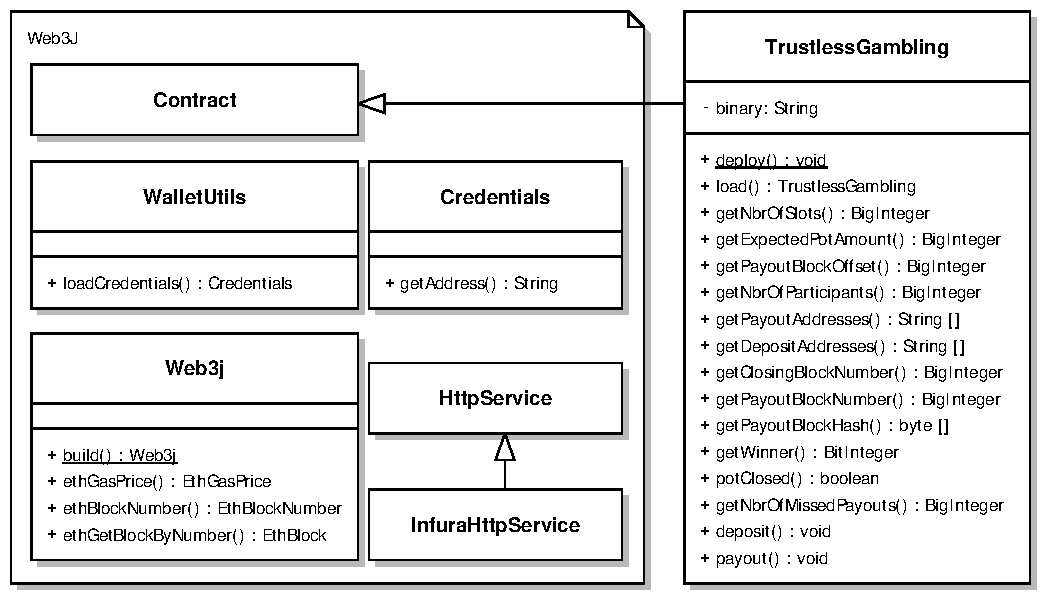
\includegraphics[width=1\linewidth]{Figures/umsetzung_eth/eth_web3j}
\decoRule
\caption{Klassendiagramm Web3J}
\label{fig:eth_web3j}
\end{figure}

Der folgende Java Code sorgt dafür, dass der von Web3J angesprochene Full-Node den Smart Contract in einer Transaktion an das Rinkeby Testnetz sendet.

\begin{lstlisting}[basicstyle=\small]
public void createContract() throws Exception {
  String WALLET_FILENAME = "ethereum.json";
  String WALLET_PASSWORD = "changeit";
  long GAS_LIMIT = 1000000;
  ClassLoader classLoader = getClass().getClassLoader();
  File walletFile = new File(classLoader.getResource(WALLET_FILENAME).getFile());
  Credentials credentials = WalletUtils.loadCredentials(WALLET_PASSWORD, walletFile.getAbsolutePath());
  System.out.println("Account address = " + credentials.getAddress());
  Web3j web3j = Web3j.build(new InfuraHttpService("https://rinkeby.infura.io/" + UserConfiguration.API_KEY));
  BigInteger currentGasPrice = web3j.ethGasPrice().send().getGasPrice();
  TrustlessGambling contract = TrustlessGambling.deploy(web3j, credentials, currentGasPrice, BigInteger.valueOf(GAS_LIMIT)).send();
  String status = contract.getTransactionReceipt().get().getStatus();
  if ("0x1".equals(status)) {
    String address = contract.getContractAddress();
    System.out.println("Contract address = " + address);
    System.out.println("TXN hash = " + contract.getTransactionReceipt().get().getTransactionHash());
    System.out.println("Gas used = " + contract.getTransactionReceipt().get().getGasUsed());
  } else {
    System.out.println("Smart contract could not be deployed.");
  }
}
\end{lstlisting}

In Zeile 5 wird der Web3J Service erzeugt. Dieser kümmert sich um die Kommunikation mit dem Full-Node. Die übergebene URL legt die Adresse des Full-Nodes fest. Infura\footnote{\url{https://infura.io/}} ist dabei ein Service, der sich auf das Hosting von Ethereum Full-Nodes spezialisiert hat. Mit Hilfe eines API Schlüssels kann man sich zu seinem Full-Node verbinden. Statt des von Infura betriebenen Nodes kann man auch einen eigens betriebenen Full-Node verwenden. Dies hat den Vorteil, dass man die volle Kontrolle behält. In diesem Fall verwendet man statt der \code{InfuraHttpService} Klasse direkt die Oberklasse \code{HttpService}.
Zeile 6 fragt den Full-Node nach dem aktuell zu bezahlenden Gaspreis.
Zeile 8 lädt die durch die Web3J Comandline Tools erzeugte Wallet. Mithilfe dieser werden unter Zuhilfenahme des Passworts die im nächsten Schritt verwendeten \code{Credentials} geladen.
In Zeile 11 wird der Smart Contract durch den Aufruf der statischen \code{deploy} Methode in einer Transaktion an das Netzwerk gesendet. Dabei wird ein Gaslimit von einer Million WEI festgelegt.
Die Ausführung des oben gezeigten Java Codes führt zu der folgenden Ausgabe:

\begin{verbatim}
Account address = 0x2201f3919589b519135ce977cc0906c9481069b2
Contract address = 0x25c3136145fbd7f3b9217e58e2fabe3eb1928705
TXN hash = 0x06dce3c460b4caa595c5cc0f81ac78e7c70eeb1e89d3e0ea88e60dbce1
Gas used = 825846
\end{verbatim}

Das Gaslimit von einer Million WEI hat ausgereicht und der Smart Contract befindet sich nun in der Blockchain des Rinkeby Testnetzes. In einem Blockchain Explorer kann man die Details der Transaktion\footnote{\url{https://rinkeby.etherscan.io/tx/0x06dce3c460ac78e7c70eeb1e89d3e0e6a017ea88e60dbce1}} und den kompilierten Contract Code\footnote{\url{https://rinkeby.etherscan.io/address/0x25c3136145fbd7f3b9217e58e2fabe3eb1928705}} anschauen.
\if Alternativ zu Web3J lässt sich der Contract Code mithilfe des Ethereum Clients namens Mist\footnote{\url{https://github.com/ethereum/mist}} veröffentlichen.
\fi

\subsection{Geschäftslogik Glücksspielanwendung}

Die Glücksspielanwendung zeigt lediglich den aktuellen Zustand des Smart Contracts an. Die gesamte Geschäftslogik des Smart Contracts wird vom Etherem Netzwerk ausgeführt. Sollte die Glücksspielanwendung aufgrund technischer Fehler ausfallen, hat dies keinerlei Auswirkung auf das eigentliche Spiel. Die Geschäftslogik der Glücksspielanwendung fragt lediglich in regelmäßigen Abständen beim Full-Node an, ob eine Änderung des Smart Contract Zustands stattgefunden hat. Abbildung \ref{fig:eth_business_logic1} liefert einen ersten Überblick über die dazu verwendeten Klassen.

\begin{figure}[H]
\centering
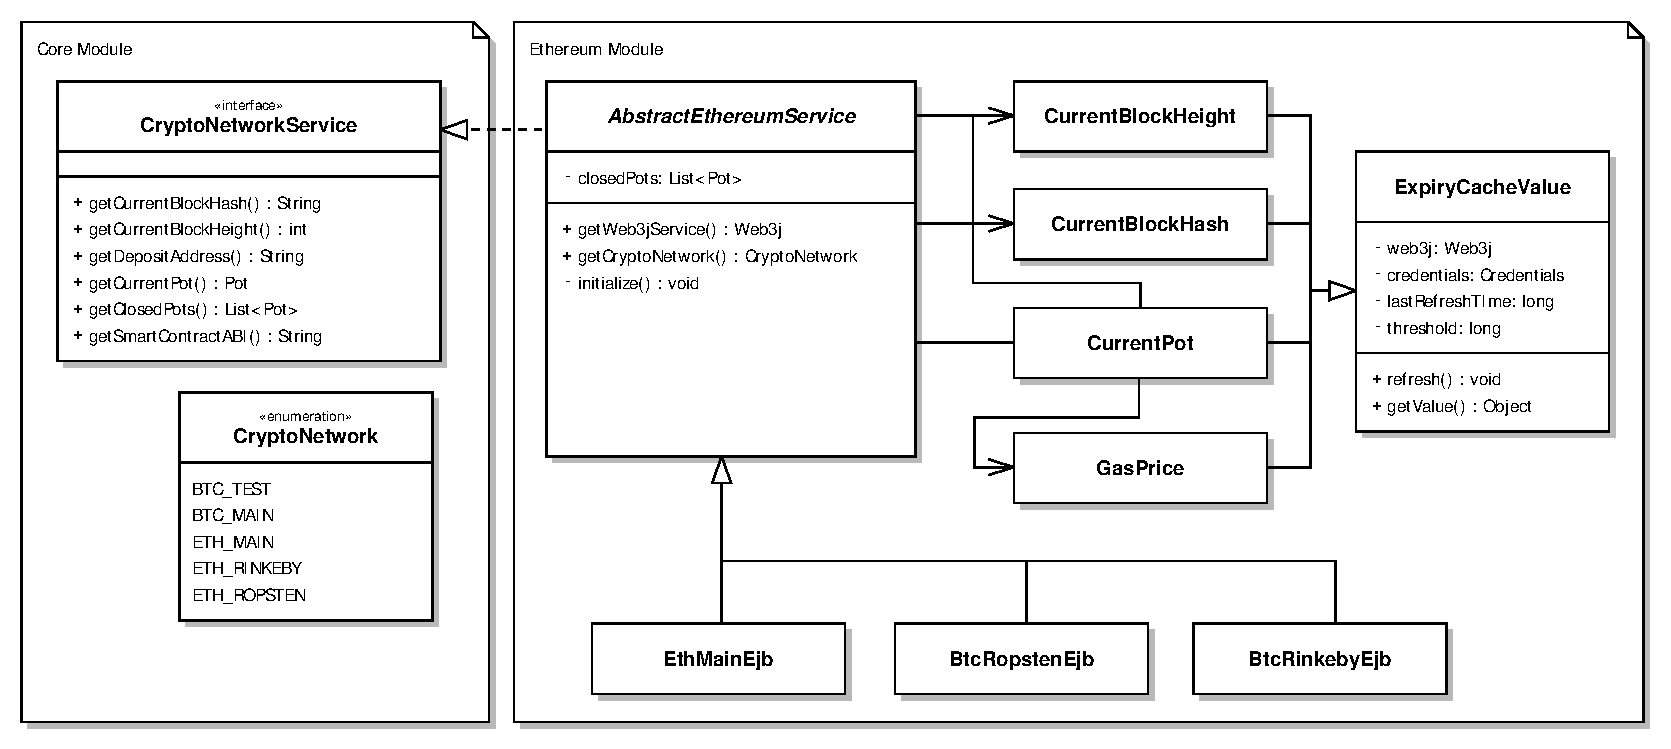
\includegraphics[width=1\linewidth]{Figures/umsetzung_eth/eth_business_logic1}
\decoRule
\caption{Klassendiagramm Ethereum}
\label{fig:eth_business_logic1}
\end{figure}

\subsubsection{Core Module}
Das \code{CryptoNetworkService} Interface wurde um die Methode \code{getSmartContractABI} erweitert. Bei dem  Smart Contract \textbf{A}pplication \textbf{B}inary \textbf{I}nterface handelt es sich um die statische zur Compile-Zeit bestimmte Schnittstellenbeschreibung, die festlegt wie man mit dem Smart Contract interagieren kann. Das Smart Contract ABI wird üblicherweise im JSON Format angegeben.

Zu dem \code{CryptoNetwork} Enum sind nun die zusätzlichen Werte \code{ETH\_MAIN},\\\code{ETH\_RINKEBY}, \code{ETH\_ROPSTEN} hinzugekommen. Über diese Werte kann man steuern mit welchem Ethereum Netzwerk die Anwendung kommunizieren soll.\\
Die Klassen \code{Pot} und \code{Participant} haben sich nicht verändert.
\subsubsection{Ethereum Module: AbstractEthereumService}

Die abstrakte Klasse \code{AbstractEthereumService} implementiert die \code{CryptoNetwork} \code{Service} Schnittstelle. Die Klassen \code{EthMainEjb, EthRopstenEjb und EthRinkebyEjb} legen lediglich über den verwendeten Web3J Service fest, welches Netzwerk die Anwendung ansprechen soll.
Die abstrakte Klasse \code{AbstractEthereumService} implementiert alle vom \code{CryptoNetworkService} Interface geforderten Methoden. Die Methoden \code{getDepositAdress} und \code{getSmartContractABI} geben lediglich die statische Smart Contract Adresse und den Smart Contract ABI JSON String zurück. Die Methoden \code{getCurrentBlockHash}, \code{getCurrentBlockHeight} und \code{getCurrentPot} geben gecachte Werte des jeweiligen \code{ExpieryCacheValue}s durch den Aufruf der \code{getValue} Methode an die Webanwendung zurück. Die Klassen \code{CurrentBlockHeight}, \code{Current} \code{BlockHash}, \code{GasPrice} und \code{CurrentPot} erweitern die abstrakte \code{ExpieryCacheValue} Klasse. Diese sorgt dafür, dass die Werte erst nach dem Ablauf einer gewissen konfigurierbaren Zeit (\code{threshold}) automatisch neu beim Full-Node angefragt werden. Dies verhindert, dass der Full-Node durch zu viele Anfragen überlastet wird. Alle Cache-Werte werden in der \code{initialize} Methode der \code{AbstractEthereumService} Klasse initialisiert. 
\begin{lstlisting}[basicstyle=\small]
@PostConstruct
private void initialize() {
  log.info("#### start " + getClass().getSimpleName() + " network service ####");
  blockHightCache = new CurrentBlockHeight(getWeb3jService(), getCredentials());
  log.info("blockHight=" + blockHightCache.getValue().intValue());
  blockHashCache = new CurrentBlockHash(getWeb3jService(), getCredentials(), blockHightCache);
  log.info("blockHash=" + blockHashCache.getValue());
  gasPriceCache = new GasPrice(getWeb3jService(), getCredentials());
  log.info("gasPrice=" + gasPriceCache.getValue().intValue());
  currentPotCache = new CurrentPot(getWeb3jService(), getCredentials(), gasPriceCache, blockHightCache,
  		UserConfiguration.CONTRACT_ADDRESS);
  log.info("currentPot=" + currentPotCache.getValue().toString());
}
\end{lstlisting}



\subsubsection{Ethereum Module: CurrentBlockHash}

Der folgende Code zeigt beispielhaft die Implementierung des \code{CurrentBlockHash ExpieryCacheValue}.

\begin{lstlisting}[basicstyle=\small]
public class CurrentBlockHash extends ExpiryCacheValue {

  CurrentBlockHeight blockHeight;

  public CurrentBlockHash(Web3j web3j, Credentials credentials, CurrentBlockHeight blockHeight) {
    super(web3j, credentials, 5 * SECOND);
    this.blockHeight = blockHeight;
  }

  /**
   * refresh if cache value expired. Called automatically by the ExpiryCacheValue.getValue()
   * method.
   */
  @Override
  protected void refresh() {
    String blockHash = fetchCurrentBlockHash();
    if (blockHash != null)
      setValue(blockHash);
  }

  private String fetchCurrentBlockHash() {
    String result = "error";
    DefaultBlockParameterNumber number = new DefaultBlockParameterNumber(blockHeight.getValue());;
    try {
      EthBlock ethBlock = getWeb3jService().ethGetBlockByNumber(number, false).send();
    result = ethBlock.getBlock().getHash();
    } catch (IOException e) {
      e.printStackTrace();
    }
    return result;
  }
}
\end{lstlisting}



In Zeile 6 wird konfiguriert, dass der aktuelle Blockhash maximal alle 5 Sekunden vom Full Node abgefragt wird. In Zeile 18 wird der neuste Block durch den Aufruf der \code{ethGetBlockByNumber} Methode angefragt. Über den Wahrheitswert-Parameter kann man entweder die gesamten Blockdaten oder nur die Header-Informationen beim Full-Node anfragen.

\subsubsection{Ethereum Module: CurrentBlockHeight}
Die Implementierung des \code{CurrentBlockHeight ExpieryCacheValue}s greift auf die folgenden Zeilen Code zurück. Es findet maximal alle 5 Sekunden eine Anfrage an den Full-Node statt.

\begin{lstlisting}[basicstyle=\small]
EthBlockNumber ethBlockNumber = getWeb3jService().ethBlockNumber().send();
BigInteger currentBlockNumber = ethBlockNumber.getBlockNumber();
\end{lstlisting}

\subsubsection{Ethereum Module: GasPrice}

Die Implementierung des \code{GasPrice ExpieryCacheValue}s greift auf die folgenden Zeilen Code zurück. Es findet maximal alle 60 Sekunden eine Anfrage an den Full-Node statt.

\begin{lstlisting}[basicstyle=\small]
EthGasPrice ethGasPrice = getWeb3jService().ethGasPrice().send();
BigInteger gasPrice = ethGasPrice.getGasPrice();
\end{lstlisting}


\subsubsection{Ethereum Module: CurrentPot}

Der \code{CurrentPot ExpieryCacheValue} verwendet die Klasse \code{TrustlessGambling} um den Zustand des Smart Contracts zu erfassen und durch die Klasse \code{Pot} abzubilden. Im Konstruktor des \code{CurrentPot ExpieryCacheValue}s wird die Methode \code{createEmptyPot} aufgerufen.

\begin{lstlisting}[basicstyle=\small]
private Pot createEmptyPot() throws Exception{
    TrustlessGambling contract = TrustlessGambling.load(contractAddress, getWeb3jService(),
            getCredentials(), gasPrice.getValue(), BigInteger.valueOf(5300000));
    int nbrOfSlots = contract.NBR_OF_SLOTS().send().intValue();
    long amount = contract.EXPECTED_POT_AMOUNT().send().longValue();
    return new Pot(nbrOfSlots, amount);
}
\end{lstlisting}



Diese Methode fragt den Full-Node, wie viele Spieler und welcher Einzahlungsbetrag vom Smart Contract erwartet wird und erzeugt anschließend einen neuen leeren Topf. Der Zustand des Topfs wird durch den folgenden Code jedes Mal aktualisiert, wenn die \code{refresh} Methode des \code{ExpieryCacheValue}s aufgerufen wird. Dies findet alle 10 Sekunden statt.

\input{CodeSnippets/eth/currentPot.tex}

Der Code unterscheidet zwischen der Anzahl Teilnehmer, die die Glücks\-spiel\-anwendung lokal zwischenspeichert (Zeile 4) und der Anzahl Teilnehmer des Datenfeldes des Smart Contracts (Zeile 5). Wenn neue Teilnehmer durch den Aufruf der \code{deposit} Methode in den Smart Contract einzahlen, wird der Topf durch die Zeilen 7 bis 11 aktualisiert. Die Ein- und Auszahlungsadressen der neuen Teilnehmer werden dazu aus den Smart Contract Daten geladen.
Durch die letzte Einzahlung wechselt der Smart Contract in den Status \code{closed}. Ab diesem Moment wird der Topf durch die Abarbeitung des Codes ab Zeile 30 aktualisiert. Zunächst werden die finalen \code{closingBlockNumber} und \code{payoutBlockNumber} Werte aus den Smart Contract Daten geladen und die \code{currentBlockNumber} durch den Full-Node bestimmt. Anschließend wird zwischen 3 Fällen unterschieden:
\begin{enumerate}
\item Zeile 38: Der zur Gewinnerauswahl benötigte Block wurde noch nicht gefunden. Dies bedeutet, dass ein Aufruf der \code{payout} Methode noch nicht möglich ist.
\item Zeile 43: Der zur Gewinnerauswahl benötigte Block wurde gefunden und die \code{payout} Methode kann aufgerufen werden. In diesem Fall wird dem Benutzer angezeigt, wie viel Zeit er noch für den Aufruf der \code{payout} Methode hat. 
\item Zeile 46: Der zur Gewinnerauswahl benötigte Block wurde zwar gefunden, es sind allerdings bereits mehr als 256 Blöcke zwischen der letzten Einzahlung und dem aktuellen Zeitpunkt vergangen. Der Smart Contract wird bei dem Aufruf der \code{payout} Methode nicht auf den Blockhash für die Gewinnerauswahl zugreifen können. Der Gewinn wird zum nächsten Topf hinzugefügt.
\end{enumerate}
Durch den Aufruf der \code{payout} Methode wird das Datenfeld, das die Anzahl der aktuellen Teilnehmer des Smart Contracts speichert, auf den Wert Null gesetzt. Da der lokal gespeicherte Topf aber noch alle Teilnehmer enthält, hat dies zur Folge, dass beim erneuten Aufruf der \code{refresh} Methode des \code{CurrenPot ExpieryCacheValue} die Bedingung aus Zeile 6 verletzt ist und der Code von Zeile 13 bis 27 ausgeführt wird. Diese Codezeilen laden den Gewinner und den \code{payoutBlockHash} aus den Daten des Smart Contracts. Wenn der \code{payoutBlockHash} den Wert \code{Null} hat, wurde die \code{payout} Methode zu spät aufgerufen. Nur in diesem Fall gibt es keinen Gewinner. Anschließend wird der aktuelle Topf zur Liste der abgearbeiteten Töpfe hinzugefügt und ein neuer Topf durch den Aufruf der \code{createEmptyPot} Methode erzeugt.
\newpage

\subsection{Grafische Benutzeroberfläche}
Das folgende Beispiel betrachtet einen frisch auf dem Ethereum Rinkeby Testnetzwerk bereitgestellten Smart Contract.

\begin{figure}[H]
\centering
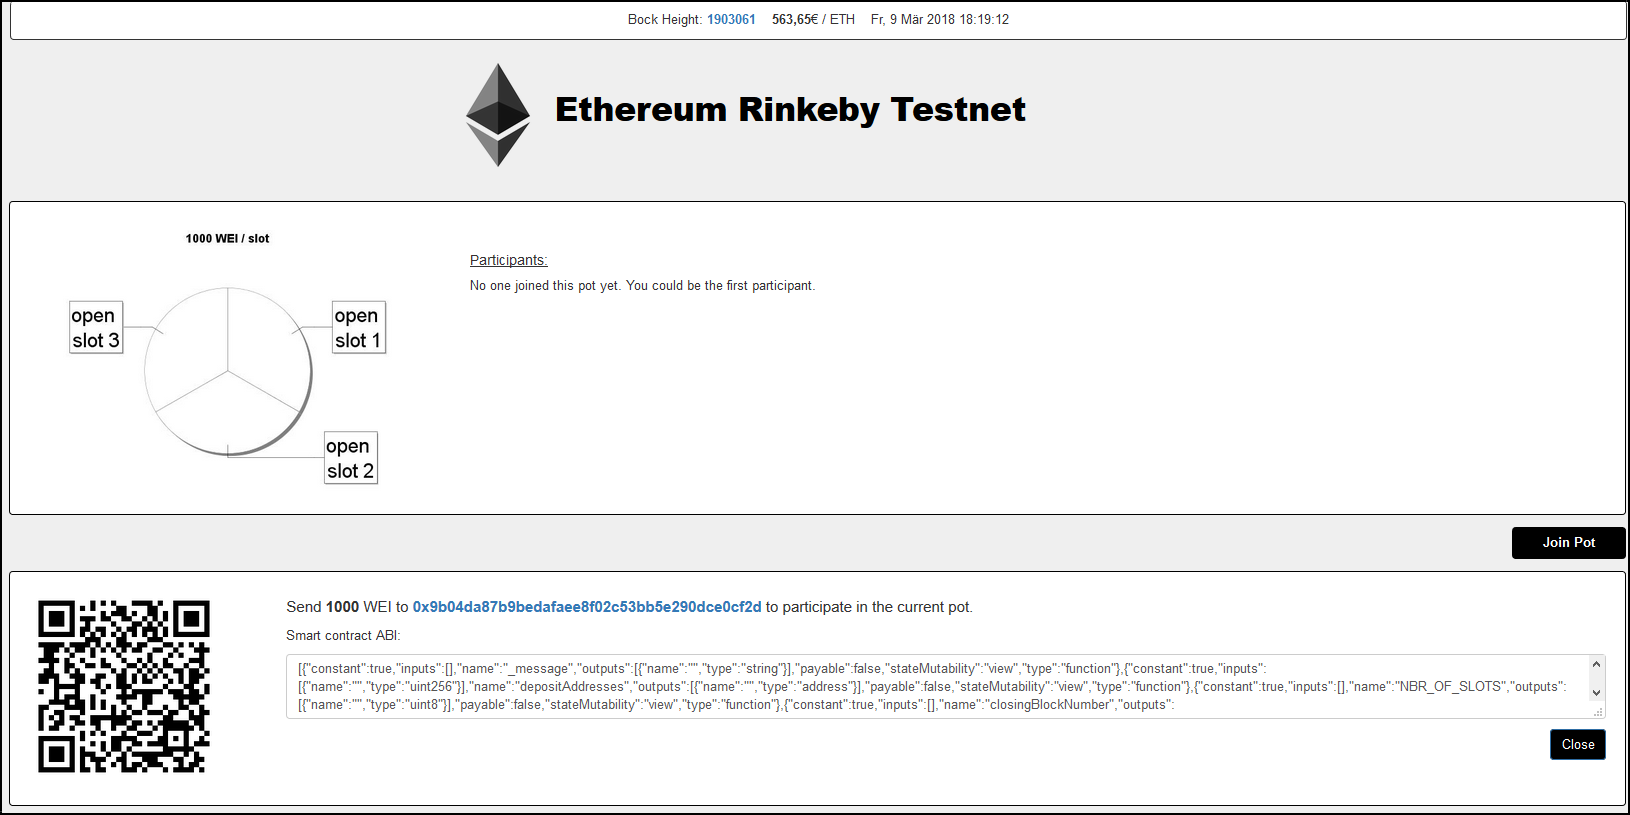
\includegraphics[width=1\linewidth]{Figures/eth_gui/ETH_pot_empty}
\decoRule
\caption{Leerer Topf}
\label{fig:ETH_pot_empty}
\end{figure}
\noindent Abbildung \ref{fig:ETH_pot_empty} zeigt einen Topf mit 3 freien Plätzen. Um dem Spiel beizutreten, muss der Spieler den Betrag von 1000 WEI an den Smart Contract senden. Genau wie bei Bitcoin wird dem Nutzer ein QR-Code angezeigt. Das \textbf{E}thereum \textbf{I}mprovement \textbf{P}roposal Nummer 681 \cite{eip681} legt die Kodierung der Daten fest.
Folgende Daten sind im QR Code enthalten:\\ ''ethereum:0x9b04da87b9bedafaee8f02c53bb5e290dce0cf2d/deposit?value=1000''. In diesem Beispiel verwenden wir für die Interaktion mit dem Netzwerk keinen Smartphone Client sondern die Webanwendung namens ''My Ether Wallet''\footnote{\url{https://www.myetherwallet.com/\#contracts}}. Diese benötigt für die Interaktion mit dem Smart Contract sowohl die Contract Adresse als auch das \textbf{A}pplication \textbf{B}inary \textbf{I}nterface.


\begin{figure}[H]
\centering
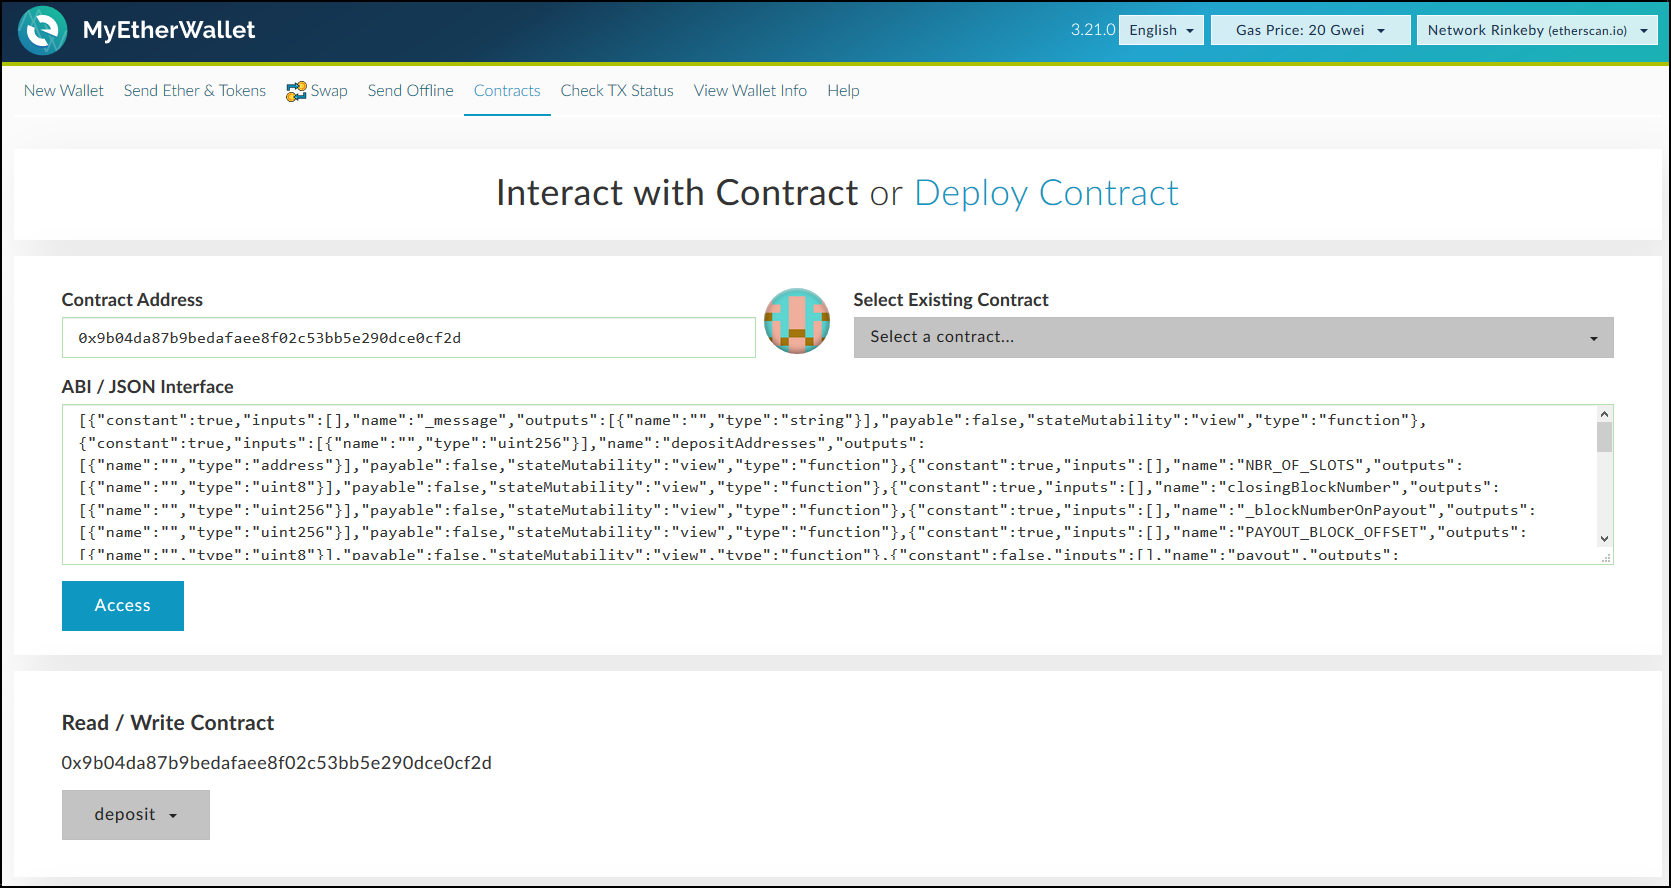
\includegraphics[width=1\linewidth]{Figures/eth_gui/ETH_wallet}
\decoRule
\caption{My Ether Wallet}
\label{fig:ETH_wallet}
\end{figure}

\noindent Nachdem der Nutzer das JSON-ABI wie in Abbildung \ref{fig:ETH_wallet} eingegeben hat, kann er über eine Dropdown-Liste die gewünschte Funktion des Smart Contracts aufrufen.


\begin{figure}[H]
\centering
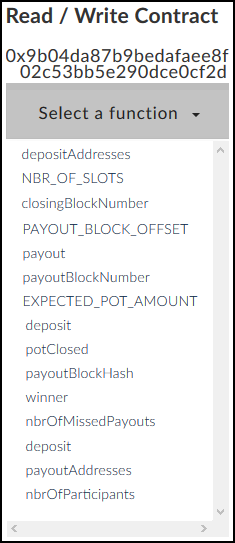
\includegraphics[scale=0.80]{Figures/eth_gui/ETH_wallet_contract_functions}
\decoRule
\caption{Liste aller Smart Contract Funktionen}
\label{fig:ETH_wallet_contract_functions}
\end{figure}

\noindent Abbildung \ref{fig:ETH_wallet_expected_amount} zeigt den Aufruf der Funktion, die die Höhe des vom Spieler erwarteten Geldbetrags zurückgibt.

\begin{figure}[H]
\centering
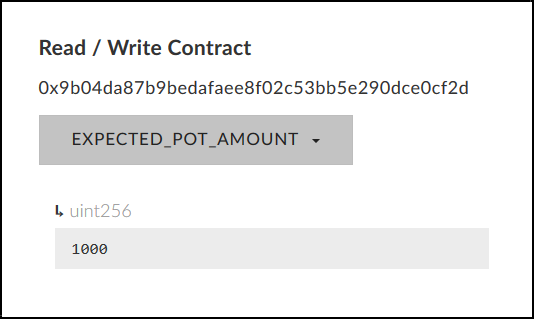
\includegraphics[scale=0.65]{Figures/eth_gui/ETH_wallet_expected_amount}
\decoRule
\caption{Aufruf der \code{EXPECTED\_POT\_AMOUNT} Funktion}
\label{fig:ETH_wallet_expected_amount}
\end{figure}

\noindent Da es sich lediglich um einen lesenden Zugriff handelt, wird keine Transaktion ans Netzwerk gesendet, beziehungsweise in die Blockchain geschrieben. Es fallen somit keine Transaktionskosten an.

\begin{figure}[H]
\centering
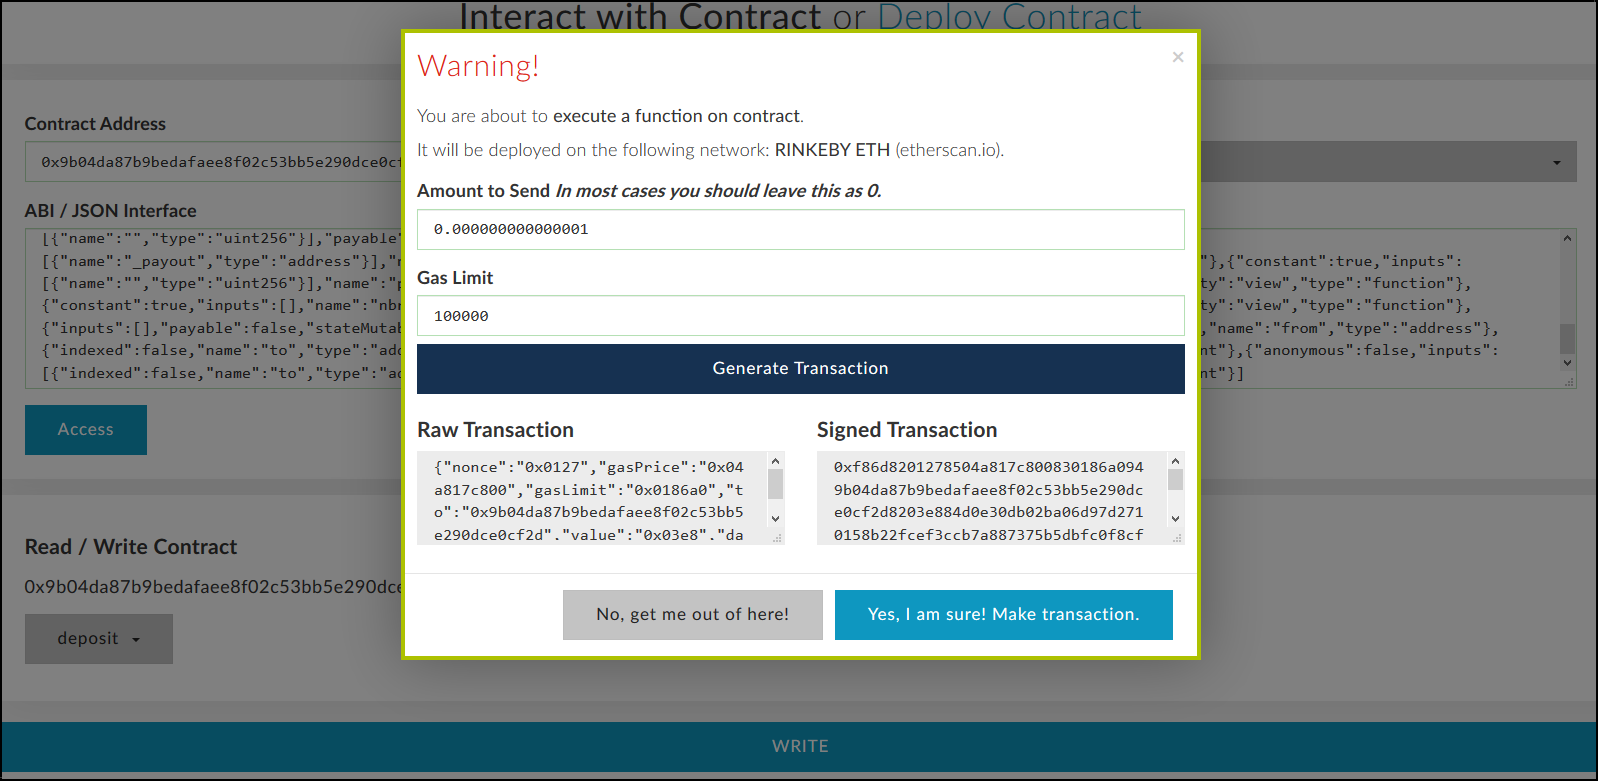
\includegraphics[width=1\linewidth]{Figures/eth_gui/ETH_wallet_deposit}
\decoRule
\caption{Aufruf der \code{deposit} Funktion}
\label{fig:ETH_wallet_deposit}
\end{figure}

\noindent Da der Nutzer nun nachgeprüft hat, dass der Smart Contract wirklich Zahlungen von 1000 WEI erwartet, kann er die \code{depsoit} Funktion mit diesem Betrag aufrufen.
Die Webseite erwartet den Betrag in der Einheit Ether. Die geforderten 1000 WEI entsprechen 0.000000000000001 Ether. Die Umrechnung kann der Spieler mittels eines Online-Konverters\footnote{\url{https://etherconverter.online/}} durchführen.
Nun muss die erstellte Transaktion nur noch signiert werden. Der Nutzer kann der Webseite dazu seinen privaten Schlüssel mitteilen oder die Signierung eigenständig durch ein sogenanntes Hardware Wallet durchführen. Die Herausgabe seines privaten Schlüssels an eine Webseite ist aus sicherheitstechnischer Sicht keine gute Praktik. Sollte der Webseitenbetreiber böse Absichten haben oder die Webseite gehackt werden, führt dies zum Verlust des durch den Schlüssel kontrollierten Geldes. Eine sichere Variante ist die Verwendung eines Hardware Wallets. Dieses speichert alle privaten Schlüssel und führt die Signatur eigenständig durch. Der verwendete private Schlüssel verlässt somit niemals das Gerät. 

\begin{figure}[H]
\centering
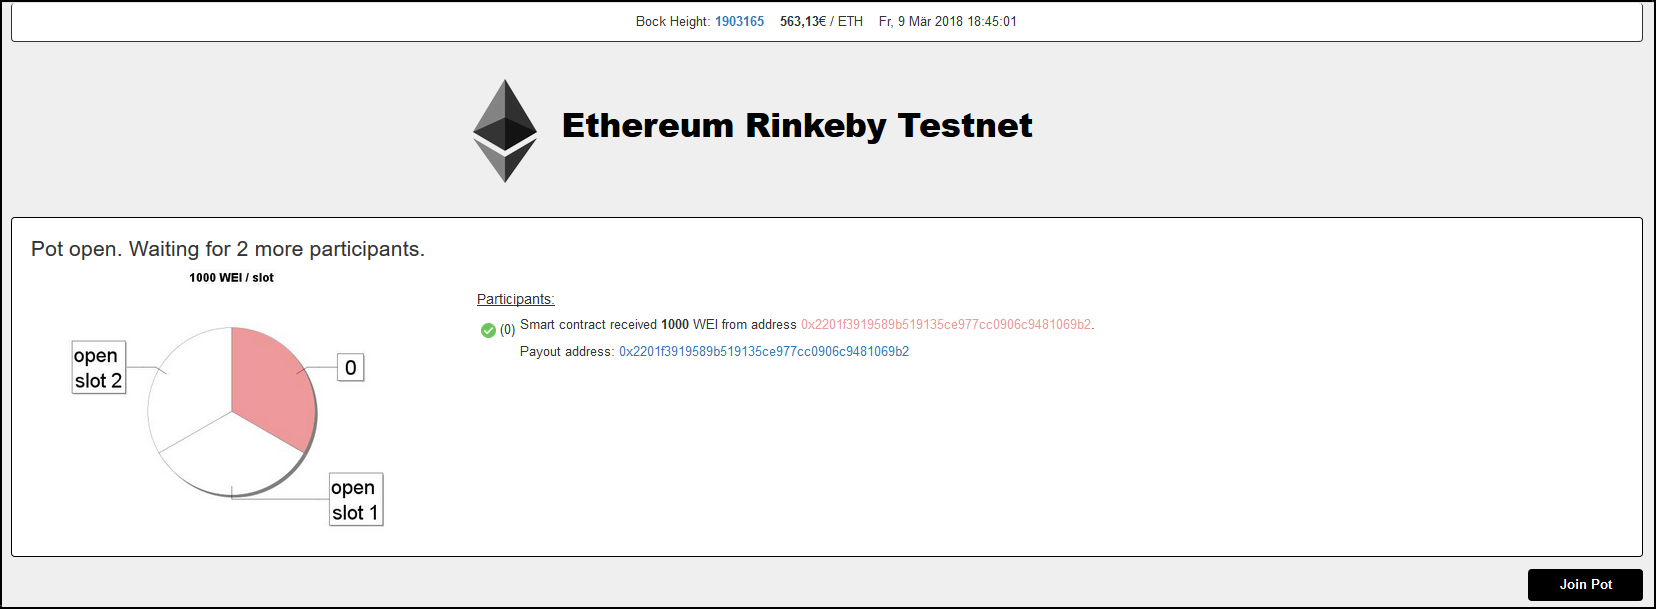
\includegraphics[width=1\linewidth]{Figures/eth_gui/ETH_pot_1}
\decoRule
\caption{Eingang der ersten Zahlung}
\label{fig:ETH_pot_1}
\end{figure}

\noindent Abbildung \ref{fig:ETH_pot_1} visualisiert den Zustand des Smart Contracts nachdem die erste Einzahlungstransaktion in die Blockchain aufgenommen wurde.

\begin{figure}[H]
\centering
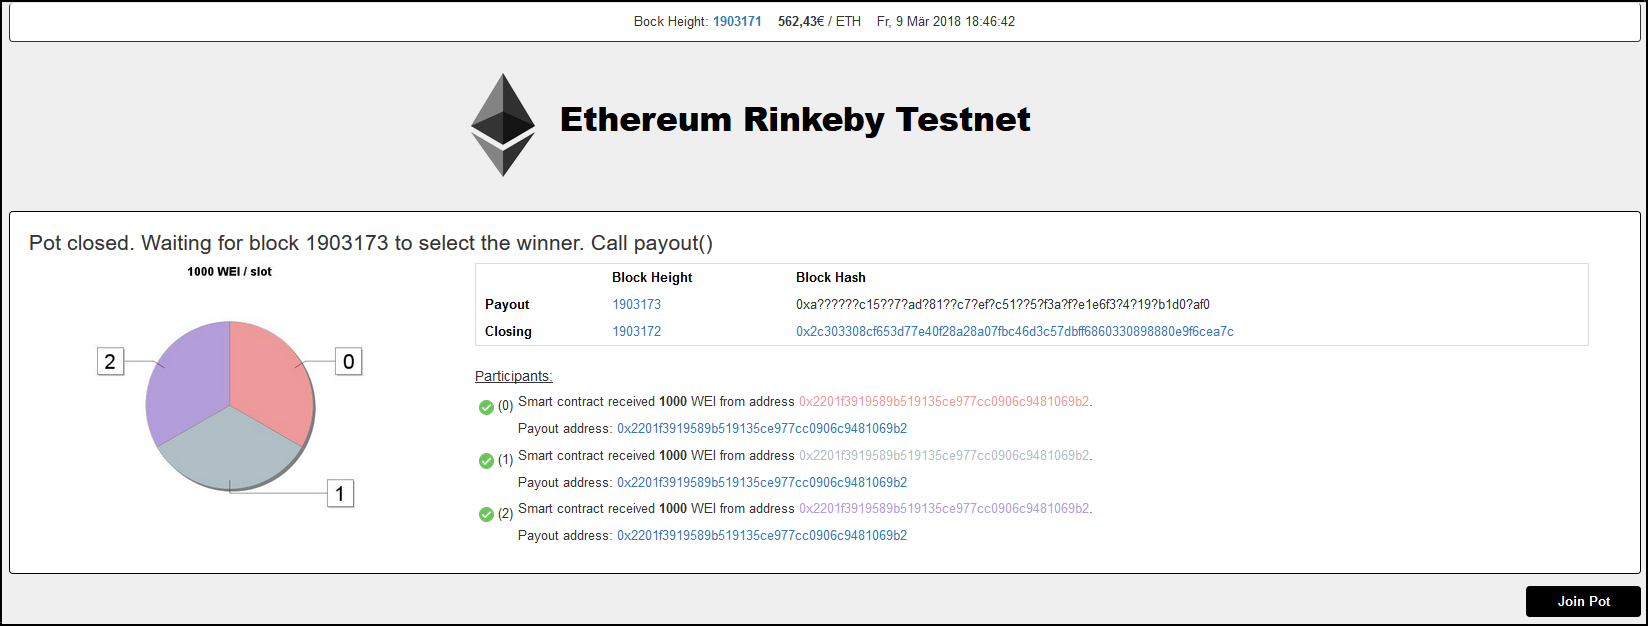
\includegraphics[width=1\linewidth]{Figures/eth_gui/ETH_pot_closed}
\decoRule
\caption{Topf geschlossen}
\label{fig:ETH_pot_closed}
\end{figure}

\noindent Abbildung \ref{fig:ETH_pot_closed} visualisiert den Zustand des Smart Contracts nachdem die letzte Einzahlungstransaktion in die Blockchain aufgenommen wurde. Der Smart Contract hat den Topf geschlossen und wartet nun, dass einer der Spieler die \code{payout} Funktion aufruft.

\begin{figure}[H]
\centering
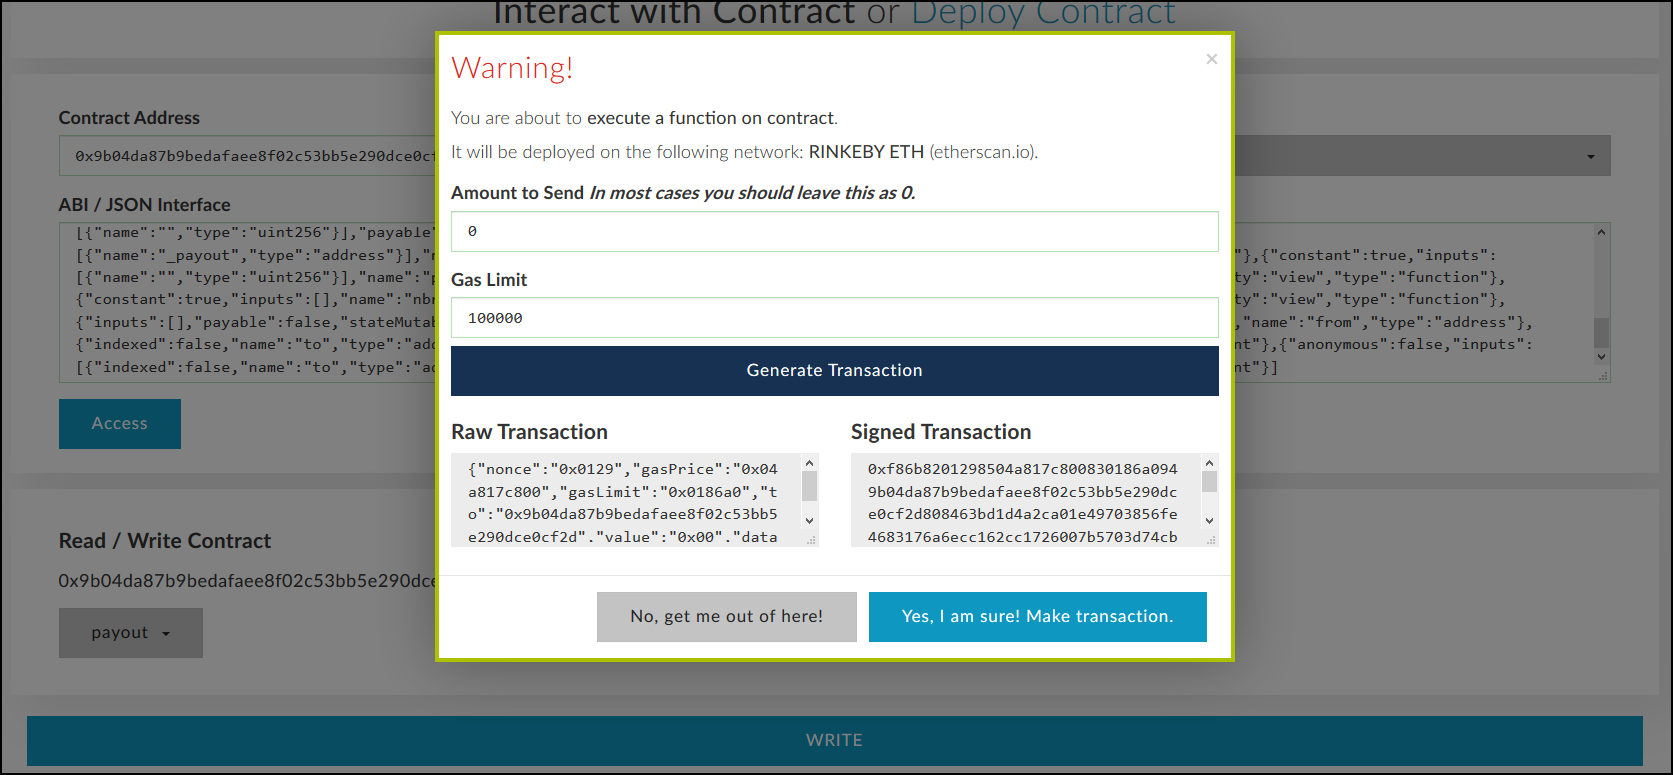
\includegraphics[width=1\linewidth]{Figures/eth_gui/ETH_wallet_payout}
\decoRule
\caption{Aufruf der \code{payout} Funktion}
\label{fig:ETH_wallet_payout}
\end{figure}

\noindent In Abbildung \ref{fig:ETH_wallet_payout} ist gezeigt wie ein Spieler die  \code{payout} Funktion aufruft. Durch den Aufruf dieser Funktion wird der Gewinner ausgewählt, die Auszahlung getätigt und der Topf wieder geöffnet.

\begin{figure}[H]
\centering
\includegraphics[width=1\linewidth]{Figures/eth_gui/ETH_pot_finished}
\decoRule
\caption{Gewinner ausgewählt}
\label{fig:ETH_pot_finished}
\end{figure}

\noindent Abbildung \ref{fig:ETH_pot_finished} zeigt den Gewinner des alten Topfs und den neu geöffneten Topf.

\begin{figure}[H]
\centering
\includegraphics[width=1\linewidth]{Figures/eth_gui/contract_transactions}
\decoRule
\caption{Block Explorer: Smart Contract}
\label{fig:contract_transactions}
\end{figure}

\noindent Abbildung \ref{fig:contract_transactions} zeigt die 3 Einzahlungstransaktionen und die Transaktion, die die \code{payout} Funktion aufruft.

\begin{figure}[H]
\centering
\includegraphics[width=1\linewidth]{Figures/eth_gui/contract_payout_txn}
\decoRule
\caption{Block Explorer: Payout Transaktion}
\label{fig:contract_payout_txn}
\end{figure}

\noindent Abbildung \ref{fig:contract_payout_txn} zeigt die Details der Transaktion, die die \code{payout} Funktion aufruft.

\section{Evaluation}
\subsection{Prüfung der Anforderungen}

Dieser Abschnitt behandelt in wie weit das beschriebene Konzept die in Anschnitt \ref{anforderungen} aufgelisteten Anforderungen erfüllt. Die jeweilige Anforderung wird zunächst wiederholt und anschließend genauer untersucht.

\subsubsection{1) Transparente Einzahlungen}
\textit{Die Einzahlung jedes Endnutzers ist für jeden anderen Endnutzer nachprüfbar.}\\\\
Einzahlungen geschehen genau wie bei Bitcoin innerhalb von Transaktionen, die in die Blockchain geschrieben werden. Diese Anforderung ist also auch im Falle von Ethereum erfüllt.
\subsubsection{2) Gewinnerauswahl durch Zufallsfaktor}
\textit{Die Auswahl des Gewinners ist von einem zufälligen Faktor abhängig, auf den weder die Anwendung noch die Endnutzer einen Einfluss haben.}\\\\
Genau wie bei Bitcoin findet die Gewinnerauswahl basierend auf einem aus dem Proof-of-Work Blockhash statt. Die in Kapitel \ref{btc_evaluation} betrachtete Analyse gilt somit genau so für Ethereum außer, dass der Mining Reward 3 Ether beträgt und durchschnittlich alle 12 Sekunden ausgeschüttet wird. In Zukunft plant Ethereum von einem Proof-of-Work Algorithmus auf einen Proof-of-Stake Algorithmus umzusteigen. Proof-of-Stake und die daraus resultierenden Auswirkungen werden in Kapitel \ref{pos} betrachtet.
\subsubsection{3) Nachprüfbarkeit des Zufallsfaktor}
\textit{Jeder Endnutzer kann die Echtheit des zufälligen Faktors eigenständig nachprüfen.}\\\\
Der zur Gewinnerauswahl verwendete Blockhash ist zum Zeitpunkt der Auszahlung bereits in der öffentlichen Blockchain verankert und kann somit überprüft werden.
\subsubsection{4) Transparente Auszahlungen}
\textit{Die Auszahlung an den Gewinner muss transparent und somit für jeden Endnutzer nachprüfbar sein.}\\\\
Die Auszahlung wird durch die vom Nutzer initiierte \code{payout} Transaktion ausgelöst und vom Smart Contract vorgenommen. Das Verfahren der Auszahlung ist durch den unveränderlichen Smart Contract Code in Stein gemeißelt. Die Konsensregeln und die dahinter liegende Spieltheorie garantieren, dass dieser auch genau so ausgeführt wird. Obwohl die \code{payout} Transaktion nicht direkt Geld auf die Auszahlungsadresse des Gewinners überweist, kann der Endnutzer dennoch sicher sein, dass eine Auszahlung stattgefunden hat, wenn die \code{payout} Transaktion wie in Abbildung \ref{fig:contract_payout_txn} im Status \code{success} vorliegt.
\subsubsection{5) Fairheit des Spiels}
\textit{Jeder Endnutzer besitzt die gleiche Gewinnwahrscheinlichkeit und niemand wird benachteiligt.}\\\\
Damit keiner der Spieler einen Vorteil hat, muss jeder Topf-Platz die gleiche Gewinnwahrscheinlichkeit haben.
Dies ist gegeben, falls jeder Teilnehmer a) die gleiche Anzahl Gewinnzahlen zugeordnet bekommt und b) falls die möglichen Blockhash-Werte für die Gewinnerauswahl gleichverteilt sind.

a) Statt wie bei Bitcoin ausschließlich die letzte Ziffer des Blockhashs für die Gewinnerauswahl zu verwenden und als Konsequenz lediglich Töpfe der Größe 2, 5 und 10 anzubieten, wird bei Ethereum der gesamte Blockhash zur Gewinnerauswahl verwendet. Dies führt zu beliebig großen Töpfen, bei denen einige Teilnehmer genau eine Gewinnzahl mehr haben können. Da jeder Spieler in der Praxis mehrere Millionen von Gewinnzahlen hat, kann man diesen theoretischen Vorteil vernachlässigen.

b) Abschnitt \ref{eth_distribution} zeigt, dass die von Ethereum eingesetzte \code{Keccak-256} Hashfunktion gleichverteilte Werte liefert.


\subsection{Aufruf der Auszahlungstransaktion}
Wie bereits in Abschnitt \ref{eth_konzept} betrachtet, ist der Aufruf deiner Funktion zur Auszahlung unumgänglich. Da der Smart Contract dies nicht selber kann, muss der Aufruf entweder von außerhalb oder von einem Anderen Smart Contract kommen.

a) Aufruf von außerhalb:\\
Der Aufruf kann wie in der Implementierung vom Gewinner ausgeführt werden. In diesem Fall zahlt der Gewinner die Transaktionsgebühr und erhält den gesamten Topf-Betrag. Der Gewinner ist dafür zuständig die Funktion rechtzeitig aufzurufen, da der Gewinn sonst in den nächsten Topf übergeht. Eine andere Möglichkeit ist es, dass die Glücksspielanwendung den Smart Contract überwacht und die \textit{payout} Funktion rechtzeitig aufruft. In diesem Fall müsste die Transaktionsgebühr von der Glücksspielanwendung gezahlt werden oder Funktionalität in den Smart Contract eingebaut werden, die die Transaktionskosten vom Topf-Betrag abzieht und der Glücksspielanwendung zurückerstattet. Allerdings verlässt sich der Gewinner dann auf die Anwendung und geht dadurch ein Risiko ein.

b) Aufruf durch Smart Contract:\\
Man kann in der Theorie den Ansatz des Ethereum Alarm Clock \footnote{\url{http://www.ethereum-alarm-clock.com/}} Contracts \footnote{\url{https://etherscan.io/address/0x6c8f2a135f6ed072de4503bd7c4999a1a17f824b}} verwenden, um eine gewünschte Smart Contract Funktion zu einem späteren Zeitpunkt auszuführen. Man spezifiziert dazu welche Funktion man wann (in welchem Blockzeitraum) ausführen möchte und zahlt für die anfallenden Transaktionsgebühren im Voraus. Dies erlaubt, dass eine ganze Reihe von Funktionen sich bei dem Alarm Clock Contract registrieren. Wird nun der Alarm Clock Contract von einem durch einen privaten Schlüssel kontrollierten Account ausgelöst, werden alle registrierten Funktionen aufgerufen. Leider liefert diese Vorgehensweise keine  Garantie, da eine registrierte Funktion nur aufgerufen wird, falls der Alarm Clock Contract aufgerufen wird. Die Glücksspielanwendung müsste also einspringen, sobald niemand anderes bereit ist den Alarm Clock Contract anzustoßen. Es handelt sich also lediglich um eine Vorgehensweise um Transaktionsgebühren mit anderen Ethereum Nutzern zu teilen.

\subsection{Verteilung der Hashfunktion Keccak-256}\label{eth_distribution}

Ethereum verwendet die kryptographische Hashfunktion Keccak-256.
Die folgende Monte-Carlo-Simulation zeigt, dass die Hashwerte der Hashfunktion Keccak-256 gleichverteilt sind.
\begin{verbatim}
h=Keccak-256 n=1000000
for i 1 -> n
    hash = h(i);
    result[uint(hash)%10]++
\end{verbatim}
\begin{minipage}{0.5\textwidth}
\begin{verbatim}
Ausgabe:
result[0] =  99227
result[1] = 100479
result[2] = 100163
result[3] =  99804
result[4] =  99945
result[5] = 100208
result[6] = 100403
result[7] = 100438
result[8] = 100035
result[9] =  99298
\end{verbatim}
\end{minipage}
\begin{minipage}{0.5\textwidth}
\includegraphics[width=\textwidth]{Figures/verteilung_keccak256}
\centering
\decoRule
\captionof{figure}{Verteilung der Keccak-256 Hashfunktion}
\label{fig:verteilung_keccak256}
\end{minipage}

\subsection{Sicherheit von Smart Contracts}
Bei Smart Contracts handelt es sich um öffentliche, für jeden ausführbare und unveränderliche Software. Beinhaltet diese einen Software Fehler, ist dieser ausnutzbar und kann nicht behoben werden. Smart Contracts verwalten in der Regel Geld oder Token, die einen finanziellen Wert repräsentieren. Bei der Entwicklung eines Smart Contracts ist somit oberste Vorsicht geboten. \todo{Hier zuerst: Durch einen kritischen Fehler im the DAO smart Contratct wurden Millionen verloren... dann erst details was the DAO ist.vllt als fussnote} Das Beispiel von the DAO zeigt, zu welchen katastrophalen Folgen Sicherheitslücken in Smart Contracts führen können.
Bei the DAO handelt es sich um einen von Christoph Jentzsch programmierten und am 20ten April 2016 auf der Ethereum Blockchain veröffentlicht Smart Contract\footnote{\url{https://etherscan.io/address/0xbb9bc244d798123fde783fcc1c72d3bb8c189413\#code}}.
The DAO ist ein Kapitalfond, der es sich zur Aufgabe gemacht hat in Blockchain Technologie zu investieren. Bei dem initialen 28zig tägigen Crowdsale wurden mehr als 150 Millionen Dollar von über 11 Tausend Investoren eingesammelt. Investoren haben Kapital in Form von Ether eingezahlt und als Gegenleistung eine entsprechende Anzahl Token als eine Art Stimmrecht erhalten. Investitionsentscheidungen dieser \textbf{d}ezentralen \textbf{a}utonomen \textbf{O}rganisation werden mithilfe des Smart Contracts durch einen dezentral erarbeiteten Konsens getroffen. Durch das Ausnutzen eines nicht trivialen Fehlers im Smart Contract Code schaffte es ein Hacker einen großen Teil des Kapitals an eine von ihm kontrollierte Adresse auszuzahlen. Eine genaue Beschreibung des Angriffes findet man unter \cite{eth_dao_hack}.

Die Solidity Dokumentation \footnote{\url{https://solidity.readthedocs.io/en/develop/security-considerations.html}} listet eine Reihe von Beispielen, die die Sicherheit von Smart Contracts betreffen. Entwickler sollten sich dieser bewusst sein, bevor sie einen Smart Contract veröffentlichen der Geld verwaltet.
\todo{Sicherheitsaspekt auf eigenen Smart Contract beziehen.}

\if
Hier dann noch darauf eingehen, dass man auf keinen Fall bock.timestamp verwenden sollte, da Miner auf diesen einen direkten Zugriff haben können.

https://ethereum.stackexchange.com/questions/19341/address-send-vs-address-transfer-best-practice-usage

Hier dann nur darauf eingehen, dass falls man die Auszahlung mittels der unsicheren Methode macht ein BUG besteht. 

Anscheinend ist bei address.transfer aber sicher, dass kein contract code ausgeführt wird. Es gibt allerdings 3 Möglichkeiten zu senden.
Eine ist unsicher.

\begin{lstlisting}[basicstyle=\small]
function payout() public{
    assert(potClosed);
    assert(block.number>payoutBlockNumber);
    potClosed = false; //fixes bug
    payoutBlockHash = block.blockhash(payoutBlockNumber); 
    if(payoutBlockHash == 0){
        nbrOfMissedPayouts++;
    }else{
        winner = uint(payoutBlockHash) % NBR_OF_SLOTS;
        address winnerAddress = payoutAddresses[winner];
        uint amount= EXPECTED_POT_AMOUNT*NBR_OF_SLOTS;
        amount += EXPECTED_POT_AMOUNT*NBR_OF_SLOTS*nbrOfMissedPayouts;
        winnerAddress.transfer(amount); // send pot amount to winner
        nbrOfMissedPayouts = 0;
    }
    nbrOfParticipants=0;
}
\end{lstlisting}


\fi


\chapter{Sonstige Distributed-Ledger-Technologie}
\section{Directed Acyclic Graph}
Bei einem DAG handelt es sich um eine gerichteten azyklischen Graphen, der im Bereich der  Distributed-Ledger-Technologie dazu eingesetzt wird Transaktionen zu speichern.
Die Kryptowährung IOTA\footnote{\url{https://www.iota.org/}} setzt solch eine Datenstruktur ein. Der Konsens entsteht nicht durch eine Blockchain auf die sich alle Teilnehmer mithilfe der Konsnensregeln einigen. Der Konsens entsteht dadurch, dass Teilnehmer neue Transaktionen nur auf Transaktionen aufbauen, die sie für gültig halten. Um eine Transaktion in den Graphen zu schreiben, muss der Absender Proof-of-Work erledigen. 

\begin{figure}[H]
\centering
\includegraphics[width=1\linewidth]{Figures/tangle}
\decoRule
\caption{Directed Acyclic Graph}
\label{fig:tangle}
\end{figure}

Die grüne Transaktion aus Abbildung \ref{fig:tangle} baut auf den beiden roten Transaktionen auf und bestätigt diese auf diese Art und Weise. Je tiefer eine Transaktion im Graphen steckt, desto mehr Proof-of-Work baut auf ihr auf. Am rechten Rand befinden sich in blau neue, unbestätigte Transaktionen.
Kryptowährungen auf Basis solch einer Datenstruktur sind nicht für die Gewinnerauswahl einer Glücksspielanwendung nutzbar, da man sich nicht bereits im Vorfeld auf ein eindeutiges, in der Zukunft liegendes, aber dennoch zufälliges Ereignis einigen kann. Weiterführende Informationen zu IOTA und einer genaue Beschreibung der DAG Datenstruktur findet man unter \citep{tangle_whitepaper}.
\section{Konsensalgorithmus: Proof of stake }\label{pos}
Hier kann man auch noch erwähnen, dass Proof of stake und solche slotbasierten Ansätze nicht geeignet sind da der Slotleader direkten Einfluss nehmen kann.
\section{Payment Channels und Lightning Network}
Hier könnte man darauf eingehen, dass off-chain Transaktionen nicht einsetzbar sind, da die restlichen Teilnehmer somit nicht die Einzahlung überprüfen können.

\chapter{Fazit} % Main chapter title
Der Einsatz von Blockchain-Technologie ermöglicht
den Austausch von digitalen finanziellen Werten zwischen sich gegenseitig misstrauenden Parteien, ohne dabei auf eine Trusted Third Party angewiesen zu sein.
Das vorher benötigte Vertrauen wird nun in ein öffentliches, transparentes System verlagert, dessen inhärente Spieltheorie den Teilnehmern finanzielle Anreize liefert, sich korrekt zu verhalten. 

Diese Arbeit hat zunächst gezeigt, wie man solche Systeme in eine eigene Anwendung integrieren kann und auf welche Besonderheiten dabei zu achten ist. 
Außerdem wurde aufgezeigt, dass man Systeme, die auf einem Proof-of-Work Konsensalgorithmus basieren, in einem gewissen Rahmen als eine verlässliche Zufallsquelle nutzen kann.
Die im ersten Ansatz entwickelte, auf der Bitcoin Blockchain aufbauende Glücksspielanwendung erlaubt es dem Nutzer die zufällige Gewinnerauswahl nachzuprüfen. Die Anwendung kann den Nutzer in dieser Hinsicht nicht benachteiligen oder betrügen. Lediglich die von der Anwendung vorzunehmende Auszahlungstransaktion an den Gewinner bietet eine gewisse Angriffsfläche. Der Endnutzer muss der Anwendung vertrauen, diese korrekt durchzuführen. Eine korrumpierte, sich falsch verhaltende Anwendung fällt dem Endnutzer allerdings auf. Ein solcher Service ist nur unter der Bedingung nutzbar, dass der Endnutzer den Betreiber des Services kennt und somit juristisch haftbar machen kann. 

Diese Problematik wurde mithilfe sogenannter Smart Contracts der Ethereum Blockchain gelöst.
Diese erlauben es dem Nutzer vollständig auf Vertrauen verzichten zu können, da die Geschäftslogik der Glücksspielanwendung in der Blockchain verankert ist und von allen Teilnehmern des Netzwerkes ausgeführt wird. Der komplette Verzicht auf Vertrauen resultiert allerdings in einer schlechteren Usability. Der Nutzer muss verstehen, welche Smart Contract Funktion er zu welchem Zeitpunkt aufrufen muss. Verpasst er den korrekten Zeitpunkt, verliert er seinen Gewinn. Dies ist bei Bitcoin nicht der Fall. Dort muss er lediglich einen QR-Code scannen und die Zahlung autorisieren.\\\\


Das Ziel von Blockchains ist es durch transparente Systeme, die Interaktionen zwischen sich misstrauenden Parteien zu ermöglichen ohne, dass dabei das Vertrauen in eine Drittpartei erforderlich ist. Das Beispiel der Glücksspielanwendung ist in so weit gelungen, da keine zusätzlichen Daten aus der echten Welt dafür benötigt werden. Im Falle von Ethereum findet die gesamte Interaktion innerhalb des Ethereum Systems statt.

Andere Anwendungsfälle wie Supply Chain, ... sind schwerer zu realisieren, da man auf Daten angewiesen ist, die aus der echten Welt in die Blockchain geschrieben werden muss. An der Schnittstelle zwischen der auf Kryptographie basierenden Blockchain Welt und der echten Welt ist es unmöglich vollständig auf Vertrauen zu verzichten.\\\\

TODO:\\
Ansprechen, dass meine Projektidee gezwungenermaßen on-chain-Transaktionen braucht, da sie sonst nicht von allen Nutzern nachvollzogen werden können. Da Bitcoin mit sehr großer Wahrscheinlichkeit weiterlebt und nicht in nächster Zukunft nicht ''stirbt'' werden bei steigendem Bedarf on-chain-Transaktionen stetig teurer. Daraus folgt dann, dass meine Idee keinen Sinn mehr für kleine Beträge macht. Hier dann nochmal darauf eingehen, dass das Lightning Network verspricht einen Großteil der Transaktionen off-cain zu bringen.



%----------------------------------------------------------------------------------------
%	THESIS CONTENT - APPENDICES
%----------------------------------------------------------------------------------------

\appendix % Cue to tell LaTeX that the following "chapters" are Appendices

% Include the appendices of the thesis as separate files from the Appendices folder
% Uncomment the lines as you write the Appendices

\chapter{Vorhandene Glücksspielseiten}
\section{Bitcoin}
Die Internetseite Crypto Games \cite{crypto_games} bietet ein Würfelspiel an, bei dem der Nutzer mit Kryptowährungen bezahlen kann. Der Spieler wettet darauf, dass der Wert einer ''zufällig'' generierten Zahl (zwischen 0 und 100) über einem bestimmten Zielwert liegt. Der Spieler kann nachdem die Wette platziert ist eigenständig prüfen, ob er gewonnen hat.
\begin{figure}[H]
\centering
\includegraphics[scale=0.5]{Figures/crypto_games}
\decoRule
\caption{MANUAL BET}
\label{fig:crypto_games}
\end{figure}

Das Formular aus Abbildung \ref{fig:crypto_games} lässt den Spieler die Höhe des Einsatzes und den Multiplikator anpassen. Je höher der Multiplikator, desto höher passt die Glücks\-spiel\-seite den Zielwert an.

Bereits bevor der Spieler die Wette abschließt, teilt ihm die Seite den SHA256 Hash des sogenannten ''Server seed'' mit. Der Server Seed ist zu diesem Zeitpunkt nur dem Service bekannt und wird erst nach dem Abschluss der Wette veröffentlicht.
Außerdem ermöglicht die Seite es dem Spieler den sogenannten ''Next client seed'' frei zu wählen. Dieser geht zusammen mit dem Server Seed in die Berechnung der Gewinnerauswahl ein. Sobald der Spieler die Wette abschließt, veröffentlicht der Service den ''Server seed''. Der Spieler kann durch die Berechnung des SHA256 Hash nachprüfen, ob es sich wirklich um den echten Wert handelt.

\begin{figure}[H]
\centering
\includegraphics[scale=0.5]{Figures/crypto_games_details}
\decoRule
\caption{PROVABLY FAIR}
\label{fig:crypto_games_details}
\end{figure}

Nun erfolgt die Gewinnerauswahl. Zunächst wird der SHA512 Hash des konkatenierten Server und Client Seeds berechnet. Dieser Hash Wert liefert die Zufallsquelle für die Gewinnerauswahl. Die ersten 5 Stellen des Hashs in Hexadezimaldarstellung werden in eine Dezimalzahl konvertiert. Anschließend werden die letzten 5 Ziffern als Zahl zwischen 0 und 100 mit 3 Nachkommastellen betrachtet. Die nachfolgende Abbildung veranschaulicht diesen Prozess.

\begin{figure}[H]
\centering
\includegraphics[scale=0.5]{Figures/crypto_games_result}
\decoRule
\caption{BET RESULT}
\label{fig:crypto_games_result}
\end{figure}

Im Beispiel aus Abbildung \ref{fig:crypto_games_result} liegt die resultierende Zahl (72,846) über dem Zielwert 50,399. Dies führt dazu, dass der Spieler gewinnt und seinen Einsatz ausgezahlt bekommt.

\section{Ethereum}

Die Internetseite \cite{vdice} bietet ein Würfelspiel an, das durch einen Smart Contract auf der Ethereum Plattform umgesetzt ist. Die Internetseite übernimmt dabei lediglich die Visualisierung der platzierten Wetten. Die Teilnahme benötigt keinen Account, da man ausschließlich mit dem Smart Contract\footnote{\url{https://etherscan.io/address/0xdd98b423dc61a756e1070de151b1485425505954\#code}} interagiert. Statt des Blockhashs wird ein sogenannter Oracle Service \cite{oracalize_it} zur Gewinnerauswahl verwendet. Dieser liefert Zufallszahlen des Services \cite{random_org} zusammen mit einer Echtheitsgarantie (Signatur) innerhalb von Transaktionen an den Smart Contract. Der Smart Contract prüft die Echtheit der Daten mittels der Signatur und führt anschließend die Gewinnerauswahl und Auszahlung durch. Detaillierte Informationen über die Funktionsweise eines Oracles und dessen Einsatzmöglichkeiten findet man unter \cite{eth_oracles}.

%----------------------------------------------------------------------------------------
%	BIBLIOGRAPHY
%----------------------------------------------------------------------------------------

\printbibliography[heading=bibintoc,title={Quellenverzeichnis}]


%----------------------------------------------------------------------------------------
%	LIST OF FIGURES/TABLES
%----------------------------------------------------------------------------------------


\listoffigures % Prints the list of figures

%\listoftables % Prints the list of tables

\listoftodos


\end{document}  
